\PassOptionsToPackage{unicode=true}{hyperref} % options for packages loaded elsewhere
\PassOptionsToPackage{hyphens}{url}
%
\documentclass[oneside,14pt,spanish,]{extbook} % cjns1989 - 27112019 - added the oneside option: so that the text jumps left & right when reading on a tablet/ereader
\usepackage{lmodern}
\usepackage{amssymb,amsmath}
\usepackage{ifxetex,ifluatex}
\usepackage{fixltx2e} % provides \textsubscript
\ifnum 0\ifxetex 1\fi\ifluatex 1\fi=0 % if pdftex
  \usepackage[T1]{fontenc}
  \usepackage[utf8]{inputenc}
  \usepackage{textcomp} % provides euro and other symbols
\else % if luatex or xelatex
  \usepackage{unicode-math}
  \defaultfontfeatures{Ligatures=TeX,Scale=MatchLowercase}
%   \setmainfont[]{EBGaramond-Regular}
    \setmainfont[Numbers={OldStyle,Proportional}]{EBGaramond-Regular}      % cjns1989 - 20191129 - old style numbers 
\fi
% use upquote if available, for straight quotes in verbatim environments
\IfFileExists{upquote.sty}{\usepackage{upquote}}{}
% use microtype if available
\IfFileExists{microtype.sty}{%
\usepackage[]{microtype}
\UseMicrotypeSet[protrusion]{basicmath} % disable protrusion for tt fonts
}{}
\usepackage{hyperref}
\hypersetup{
            pdftitle={TRAFALGAR},
            pdfauthor={Benito Pérez Galdós},
            pdfborder={0 0 0},
            breaklinks=true}
\urlstyle{same}  % don't use monospace font for urls
\usepackage[papersize={4.80 in, 6.40  in},left=.5 in,right=.5 in]{geometry}
\setlength{\emergencystretch}{3em}  % prevent overfull lines
\providecommand{\tightlist}{%
  \setlength{\itemsep}{0pt}\setlength{\parskip}{0pt}}
\setcounter{secnumdepth}{0}

% set default figure placement to htbp
\makeatletter
\def\fps@figure{htbp}
\makeatother

\usepackage{comment}

\usepackage{ragged2e}
\usepackage{epigraph}
\renewcommand{\textflush}{flushepinormal}

\usepackage{indentfirst}
\usepackage{pdfpages}

\usepackage{fancyhdr}
\pagestyle{fancy}
\fancyhf{}
\fancyhead[R]{\thepage}
\renewcommand{\headrulewidth}{0pt}
\usepackage{quoting}
\usepackage{ragged2e}

\usepackage{rotating}

\newlength\mylen
\settowidth\mylen{……………….}

\usepackage{stackengine}
\usepackage{graphicx}
\def\asterism{\par\vspace{1em}{\centering\scalebox{.9}{%
  \stackon[-0.6pt]{\bfseries*~*}{\bfseries*}}\par}\vspace{.8em}\par}

 \usepackage{titlesec}
 \titleformat{\chapter}[display]
  {\normalfont\bfseries\filcenter}{}{0pt}{\Large}
 \titleformat{\section}[display]
  {\normalfont\bfseries\filcenter}{}{0pt}{\Large}
 \titleformat{\subsection}[display]
  {\normalfont\bfseries\filcenter}{}{0pt}{\Large}

\setcounter{secnumdepth}{1}
\ifnum 0\ifxetex 1\fi\ifluatex 1\fi=0 % if pdftex
  \usepackage[shorthands=off,main=spanish]{babel}
\else
  % load polyglossia as late as possible as it *could* call bidi if RTL lang (e.g. Hebrew or Arabic)
%   \usepackage{polyglossia}
%   \setmainlanguage[]{spanish}
%   \usepackage[french]{babel} % cjns1989 - 1.43 version of polyglossia on this system does not allow disabling the autospacing feature
\fi

\title{TRAFALGAR}
\author{Benito Pérez Galdós}
\date{}

\begin{document}
\maketitle

\hypertarget{i}{%
\chapter{I}\label{i}}

Se me permitirá que antes de referir el gran suceso de que fui testigo,
diga algunas palabras sobre mi infancia, explicando por qué extraña
manera me llevaron los azares de la vida a presenciar la terrible
catástrofe de nuestra marina.

Al hablar de mi nacimiento, no imitaré a la mayor parte de los que
cuentan hechos de su propia vida, quienes empiezan nombrando su
parentela, las más veces noble, siempre hidalga por lo menos, si no se
dicen descendientes del mismo Emperador de Trapisonda. Yo, en esta
parte, no puedo adornar mi libro con sonoros apellidos; y fuera de mi
madre, a quien conocí por poco tiempo, no tengo noticia de ninguno de
mis ascendientes, si no es de Adán, cuyo parentesco me parece
indiscutible. Doy principio, pues, a mi historia como Pablos, el buscón
de Segovia; afortunadamente Dios ha querido que en esto sólo nos
parezcamos.

Yo nací en Cádiz, y en el famoso barrio de la Viña, que no es hoy, ni
menos era entonces, academia de buenas costumbres. La memoria no me da
luz alguna sobre mi persona y mis acciones en la niñez, sino desde la
edad de seis años; y si recuerdo esta fecha, es porque la asocio a un
suceso naval de que oí hablar entonces: el combate del cabo de San
Vicente, acaecido en 1797.

Dirigiendo una mirada hacia lo que fue, con la curiosidad y el interés
propios de quien se observa, imagen confusa y borrosa, en el cuadro de
las cosas pasadas, me veo jugando en la Caleta con otros chicos de mi
edad poco más o menos. Aquello era para mí la vida entera; más aún, la
vida normal de nuestra privilegiada especie; y los que no vivían como
yo, me parecían seres excepcionales del humano linaje, pues en mi
infantil inocencia y desconocimiento del mundo yo tenía la creencia de
que el hombre había sido criado para la mar, habiéndole asignado la
Providencia, como supremo ejercicio de su cuerpo, la natación, y como
constante empleo de su espíritu el buscar y coger cangrejos, ya para
arrancarles y vender sus estimadas bocas, que llaman de la Isla, ya para
propia satisfacción y regalo, mezclando así lo agradable con lo útil.

La sociedad en que yo me crié era, pues, de lo más rudo, incipiente y
soez que puede imaginarse, hasta tal punto, que los chicos de la Caleta
éramos considerados como más canallas que los que ejercían igual
industria y desafiaban con igual brío los elementos en Puntales; y por
esta diferencia, uno y otro bando nos considerábamos rivales, y a veces
medíamos nuestras fuerzas en la Puerta de Tierra con grandes y ruidosas
pedreas, que manchaban el suelo de heroica sangre.

Cuando tuve edad para meterme de cabeza en los negocios por cuenta
propia, con objeto de ganar honradamente algunos cuartos, recuerdo que
lucí mi travesura en el muelle, sirviendo de introductor de embajadores
a los muchos ingleses que entonces como ahora nos visitaban. El muelle
era una escuela ateniense para despabilarse en pocos años, y yo no fui
de los alumnos menos aprovechados en aquel vasto ramo del saber humano,
así como tampoco dejé de sobresalir en el merodeo de la fruta, para lo
cual ofrecía ancho campo a nuestra iniciativa y altas especulaciones la
plaza de San Juan de Dios. Pero quiero poner punto en esta parte de mi
historia, pues hoy recuerdo con vergüenza tan grande envilecimiento, y
doy gracias a Dios de que me librara pronto de él llevándome por más
noble camino.

Entre las impresiones que conservo, está muy fijo en mi memoria el
placer entusiasta que me causaba la vista de los barcos de guerra,
cuando se fondeaban frente a Cádiz o en San Fernando. Como nunca pude
satisfacer mi curiosidad, viendo de cerca aquellas formidables máquinas,
yo me las representaba de un modo fantástico y absurdo, suponiéndolas
llenas de misterios.

Afanosos para imitar las grandes cosas de los hombres, los chicos
hacíamos también nuestras escuadras, con pequeñas naves, rudamente
talladas, a que poníamos velas de papel o trapo, marinándolas con mucha
decisión y seriedad en cualquier charco de Puntales o la Caleta. Para
que todo fuera completo, cuando venía algún cuarto a nuestras manos por
cualquiera de las vías industriales que nos eran propias, comprábamos
pólvora en casa de la tía Coscoja de la calle del Torno de Santa María,
y con este ingrediente hacíamos una completa fiesta naval. Nuestras
flotas se lanzaban a tomar viento en océanos de tres varas de ancho;
disparaban sus piezas de caña; se chocaban remedando sangrientos
abordajes, en que se batía con gloria su imaginaria tripulación;
cubríalas el humo, dejando ver las banderas, hechas con el primer trapo
de color encontrado en los basureros; y en tanto nosotros bailábamos de
regocijo en la costa, al estruendo de la artillería, figurándonos ser
las naciones a que correspondían aquellos barcos, y creyendo que en el
mundo de los hombres y de las cosas grandes, las naciones bailarían lo
mismo presenciando la victoria de sus queridas escuadras. Los chicos ven
todo de un modo singular.

Aquélla era época de grandes combates navales, pues había uno cada año,
y alguna escaramuza cada mes. Yo me figuraba que las escuadras se batían
unas con otras pura y simplemente porque les daba la gana, o con objeto
de probar su valor, como dos guapos que se citan fuera de puertas para
darse de navajazos. Me río recordando mis extravagantes ideas respecto a
las cosas de aquel tiempo. Oía hablar mucho de Napoleón, ¿y cómo creen
ustedes que yo me lo figuraba? Pues nada menos que igual en todo a los
contrabandistas que, procedentes del campo de Gibraltar, se veían en el
barrio de la Viña con harta frecuencia; me lo figuraba caballero en un
potro jerezano, con su manta, polainas, sombrero de fieltro y el
correspondiente trabuco. Según mis ideas, con este pergenio, y seguido
de otros aventureros del mismo empaque, aquel hombre, que todos pintaban
como extraordinario, conquistaba la Europa, es decir, una gran isla,
dentro de la cual estaban otras islas, que eran las naciones, a saber:
Inglaterra, Génova, Londres, Francia, Malta, la tierra del Moro,
América, Gibraltar, Mahón, Rusia, Tolón, etc. Yo había formado esta
geografía a mi antojo, según las procedencias más frecuentes de los
barcos, con cuyos pasajeros hacía algún trato; y no necesito decir que
entre todas estas naciones o islas España era la mejorcita, por lo cual
los ingleses, unos a modo de salteadores de caminos, querían cogérsela
para sí. Hablando de esto y otros asuntos diplomáticos, yo y mis colegas
de la Caleta decíamos mil frases inspiradas en el más ardiente
patriotismo.

Pero no quiero cansar al lector con pormenores que sólo se refieren a
mis particulares impresiones, y voy a concluir de hablar de mí. El único
ser que compensaba la miseria de mi existencia con un desinteresado
afecto, era mi madre. Sólo recuerdo de ella que era muy hermosa, o al
menos a mí me lo parecía. Desde que quedó viuda, se mantenía y me
mantenía lavando y componiendo la ropa de algunos marineros. Su amor por
mí debía de ser muy grande. Caí gravemente enfermo de la fiebre
amarilla, que entonces asolaba a Andalucía, y cuando me puse bueno me
llevó como en procesión a oír misa a la Catedral vieja, por cuyo
pavimento me hizo andar de rodillas más de una hora, y en el mismo
retablo en que la oímos puso, en calidad de ex-voto, un niño de cera que
yo creí mi perfecto retrato.

Mi madre tenía un hermano, y si aquélla era buena, éste era malo y muy
cruel por añadidura. No puedo recordar a mi tío sin espanto, y por
algunos incidentes sueltos que conservo en la memoria, colijo que aquel
hombre debió de haber cometido un crimen en la época a que me refiero.
Era marinero, y cuando estaba en Cádiz y en tierra, venía a casa
borracho como una cuba y nos trataba fieramente, a su hermana de
palabra, diciéndole los más horrendos vocablos, y a mí de obra,
castigándome sin motivo.

Mi madre debió padecer mucho con las atrocidades de su hermano, y esto,
unido al trabajo tan penoso como mezquinamente retribuido, aceleró su
fin, el cual dejó indeleble impresión en mi espíritu, aunque mi memoria
puede hoy apreciarlo sólo de un modo vago.

En aquella edad de miseria y vagancia, yo no me ocupaba más que en jugar
junto a la mar o en correr por las calles. Mis únicas contrariedades
eran las que pudieran ocasionarme un bofetón de mi tío, un regaño de mi
madre o cualquier contratiempo en la organización de mis escuadras. Mi
espíritu no había conocido aún ninguna emoción fuerte y verdaderamente
honda, hasta que la pérdida de mi madre me presentó a la vida humana
bajo un aspecto muy distinto del que hasta entonces había tenido para
mí. Por eso la impresión sentida no se ha borrado nunca de mi alma.
Transcurridos tantos años, recuerdo aún, como se recuerdan las medrosas
imágenes de un mal sueño, que mi madre yacía postrada con no sé qué
padecimiento; recuerdo haber visto entrar en casa unas mujeres, cuyos
nombres y condición no puedo decir; recuerdo oír lamentos de dolor, y
sentirme yo mismo en los brazos de mi madre; recuerdo también,
refiriéndolo a todo mi cuerpo, el contacto de unas manos muy frías, pero
muy frías. Creo que después me sacaron de allí, y con estas indecisas
memorias se asocia la vista de unas velas amarillas que daban pavorosa
claridad en medio del día, el rumor de unos rezos, el cuchicheo de unas
viejas charlatanas, las carcajadas de marineros ebrios, y después de
esto la triste noción de la orfandad, la idea de hallarme solo y
abandonado en el mundo, idea que embargó mi pobre espíritu por algún
tiempo.

No tengo presente lo que hizo mi tío en aquellos días. Sólo sé que sus
crueldades conmigo se redoblaron hasta tal punto, que cansándome de sus
malos tratos, me evadí de la casa deseoso de buscar fortuna. Me fui a
San Fernando; de allí a Puerto Real. Junteme con la gente más perdida de
aquellas playas, fecundas en héroes de encrucijada, y no sé cómo ni por
qué motivo fui a parar con ellos a Medinasidonia, donde hallándonos
cierto día en una taberna se presentaron algunos soldados de Marina que
hacían la leva, y nos desbandamos, refugiándose cada cual donde pudo. Mi
buena estrella me llevó a cierta casa, cuyos dueños se apiadaron de mí,
mostrándome gran interés, sin duda por el relato que de rodillas, bañado
en lágrimas y con ademán suplicante, hice de mi triste estado, de mi
vida, y sobre todo de mis desgracias.

Aquellos señores me tomaron bajo su protección, librándome de la leva, y
desde entonces quedé a su servicio. Con ellos me trasladé a Vejer de la
Frontera, lugar de su residencia, pues sólo estaban de paso en
Medinasidonia.

Mis ángeles tutelares fueron don Alonso Gutiérrez de Cisniega, capitán
de navío, retirado del servicio, y su mujer, ambos de avanzada edad.
Enseñáronme muchas cosas que no sabía, y como me tomaran cariño, al poco
tiempo adquirí la plaza de paje del señor don Alonso, al cual acompañaba
en su paseo diario, pues el buen inválido no movía el brazo derecho y
con mucho trabajo la pierna correspondiente. No sé qué hallaron en mí
para despertar su interés. Sin duda mis pocos años, mi orfandad y
también la docilidad con que les obedecía, fueron parte a merecer una
benevolencia a que he vivido siempre profundamente agradecido. Hay que
añadir a las causas de aquel cariño, aunque me esté mal el decirlo, que
yo, no obstante haber vivido hasta entonces en contacto con la más
desarrapada canalla, tenía cierta cultura o delicadeza ingénita que en
poco tiempo me hizo cambiar de modales, hasta el punto de que algunos
años después, a pesar de la falta de todo estudio, hallábame en
disposición de poder pasar por persona bien nacida.

Cuatro años hacía que estaba en la casa cuando ocurrió lo que voy a
referir. No me exija el lector una exactitud que tengo por imposible,
tratándose de sucesos ocurridos en la primera edad y narrados en el
ocaso de la existencia, cuando cercano a mi fin, después de una larga
vida, siento que el hielo de la senectud entorpece mi mano al manejar la
pluma, mientras el entendimiento aterido intenta engañarse, buscando en
el regalo de dulces o ardientes memorias un pasajero rejuvenecimiento.
Como aquellos viejos verdes que creen despertar su voluptuosidad dormida
engañando los sentidos con la contemplación de hermosuras pintadas, así
intentaré dar interés y lozanía a los mustios pensamientos de mi
ancianidad, recalentándolos con la representación de antiguas grandezas.

Y el efecto es inmediato. ¡Maravillosa superchería de la imaginación!
Como quien repasa hojas hace tiempo dobladas de un libro que se leyó,
así miro con curiosidad y asombro los años que fueron; y mientras dura
el embeleso de esta contemplación, parece que un genio amigo viene y me
quita de encima la pesadumbre de los años, aligerando la carga de mi
ancianidad, que tanto agobia el cuerpo como el alma. Esta sangre, tibio
y perezoso humor que hoy apenas presta escasa animación a mi caduco
organismo, se enardece, se agita, circula, bulle, corre y palpita en mis
venas con acelerada pulsación. Parece que en mi cerebro entra de
improviso una gran luz que ilumina y da forma a mil ignorados prodigios,
como la antorcha del viajero que, esclareciendo la obscura cueva, da a
conocer las maravillas de la geología tan de repente, que parece que las
crea. Y al mismo tiempo mi corazón, muerto para las grandes sensaciones,
se levanta, Lázaro llamado por voz divina, y se me sacude en el pecho,
causándome a la vez dolor y alegría.

Soy joven; el tiempo no ha pasado; tengo frente a mí los principales
hechos de mi mocedad; estrecho la mano de antiguos amigos; en mi ánimo
se reproducen las emociones dulces o terribles de la juventud, el ardor
del triunfo, el pesar de la derrota, las grandes alegrías, así como las
grandes penas, asociadas en los recuerdos como lo están en la vida.
Sobre todos mis sentimientos domina uno, el que dirigió siempre mis
acciones durante aquel azaroso periodo comprendido entre 1805 y 1834.
Cercano al sepulcro, y considerándome el más inútil de los hombres, ¡aún
haces brotar lágrimas de mis ojos, amor santo de la patria! En cambio yo
aún puedo consagrarte una palabra, maldiciendo al ruin escéptico que te
niega, y al filósofo corrompido que te confunde con los intereses de un
día.

A este sentimiento consagré mi edad viril y a él consagro esta faena de
mis últimos años, poniéndole por genio tutelar o ángel custodio de mi
existencia escrita, ya que lo fue de mi existencia real. Muchas cosas
voy a contar. ¡Trafalgar, Bailén, Madrid, Zaragoza, Gerona,
Arapiles!\ldots{} De todo esto diré alguna cosa, si no os falta la
paciencia. Mi relato no será tan bello como debiera, pero haré todo lo
posible para que sea verdadero.

\hypertarget{ii}{%
\chapter{II}\label{ii}}

En uno de los primeros días de octubre de aquel año funesto (1805), mi
noble amo me llamó a su cuarto, y mirándome con su habitual severidad
(cualidad tan sólo aparente, pues su carácter era sumamente blando), me
dijo:

---Gabriel, ¿eres tú hombre de valor?

No supe al principio qué contestar, porque, a decir verdad, en mis
catorce años de vida no se me había presentado aún ocasión de asombrar
al mundo con ningún hecho heroico; pero el oírme llamar hombre me llenó
de orgullo, y pareciéndome al mismo tiempo indecoroso negar mi valor
ante persona que lo tenía en tan alto grado, contesté con pueril
arrogancia:

---Sí, mi amo; soy hombre de valor.

Entonces aquel insigne varón, que había derramado su sangre en cien
combates gloriosos, sin que por esto se desdeñara de tratar
confiadamente a su leal criado, sonrió ante mí, hízome seña de que me
sentara, y ya iba a poner en mi conocimiento alguna importante
resolución, cuando su esposa y mi ama doña Francisca entró de súbito en
el despacho para dar mayor interés a la conferencia, y comenzó a hablar
destempladamente en estos términos:

---No, no irás\ldots{} te aseguro que no irás a la escuadra. ¡Pues no
faltaba más!\ldots{} ¡A tus años y cuando te has retirado del servicio
por viejo!\ldots{} ¡Ay, Alonsito, has llegado a los setenta y ya no
estás para fiestas!

Me parece que aún estoy viendo a aquella respetable cuanto iracunda
señora con su gran papalina, su saya de organdí, sus rizos blancos y su
lunar peludo a un lado de la barba. Cito estos cuatro detalles
heterogéneos, porque sin ellos no puede representársela mi memoria. Era
una mujer hermosa en la vejez, como la Santa Ana de Murillo; y su
belleza respetable habría sido perfecta, y la comparación con la madre
de la Virgen exacta, si mi ama hubiera sido muda como una pintura.

Don Alonso, algo acobardado, como de costumbre, siempre que la oía, le
contestó:

---Necesito ir, Paquita. Según la carta que acabo de recibir de ese buen
Churruca, la escuadra combinada debe, o salir de Cádiz provocando el
combate con los ingleses, o esperarles en la bahía, si se atreven a
entrar. De todos modos, la cosa va a ser sonada.

---Bueno, me alegro---repuso doña Francisca.---Ahí están Gravina,
Valdés, Cisneros, Churruca, Alcalá Galiano y Álava. Que machaquen duro
sobre esos perros ingleses. Pero tú estás hecho un trasto viejo, que no
sirves para maldita de Dios la cosa. Todavía no puedes mover el brazo
izquierdo que te dislocaron en el cabo de San Vicente.

Mi amo movió el brazo izquierdo con un gesto académico y guerrero, para
probar que lo tenía expedito. Pero doña Francisca, no convencida con tan
endeble argumento, continuó chillando en estos términos:

---No, no irás a la escuadra, porque allí no hacen falta estantiguas
como tú. Si tuvieras cuarenta años, como cuando fuiste a la Tierra del
Fuego y me trajiste aquellos collares verdes de los indios\ldots{} Pero
ahora\ldots{} Ya sé yo que ese calzonazos de Marcial te ha calentado los
cascos anoche y esta mañana, hablándote de batallas. Me parece que el
señor Marcial y yo tenemos que reñir\ldots{} Vuélvase él a los barcos si
quiere, para que le quiten la pierna que le queda\ldots{} ¡Oh, San José
bendito! Si en mis quince hubiera sabido yo lo que era la gente de
mar\ldots{} ¡Qué tormento! ¡Ni un día de reposo! Se casa una para vivir
con su marido, y a lo mejor viene un despacho de Madrid que en dos
palotadas me lo manda qué sé yo a dónde, a la Patagonia, al Japón o al
mismo infierno. Está una diez o doce meses sin verle, y al fin, si no se
le comen los señores salvajes, vuelve hecho una miseria, tan enfermo y
amarillo que no sabe una qué hacer para volverle a su color
natural\ldots{} Pero pájaro viejo no entra en jaula, y de repente viene
otro despachito de Madrid\ldots{} Vaya usted a Tolón, a Brest, a
Nápoles, acá o acullá, donde le da la gana al bribonazo del Primer
Cónsul\ldots{} ¡Ah! si todos hicieran lo que yo digo, ¡qué pronto las
pagaría todas juntas ese caballerito que trae tan revuelto al mundo!

Mi amo miró sonriendo una mala estampa clavada en la pared, y que,
torpemente iluminada por ignoto artista, representaba al Emperador
Napoleón, caballero en un corcel verde, con el célebre redingote
embadurnado de bermellón. Sin duda la impresión que dejó en mí aquella
obra de arte, que contemplé durante cuatro años, fue causa de que
modificara mis ideas respecto al traje de contrabandista del grande
hombre, y en lo sucesivo me lo representé vestido de cardenal y montado
en un caballo verde.

---Esto no es vivir---continuó doña Francisca agitando los
brazos.---Dios me perdone; pero aborrezco el mar, aunque dicen que es
una de sus mejores obras. ¡No sé para qué sirve la Santa Inquisición si
no convierte en cenizas esos endiablados barcos de guerra! Pero vengan
acá y díganme: ¿Para qué es eso de estarse arrojando balas y más balas,
sin más ni más, puestos sobre cuatro tablas que, si se quiebran, arrojan
al mar centenares de infelices? ¿No es esto tentar a Dios? ¡Y estos
hombres se vuelven locos cuando oyen un cañonazo! ¡Bonita gracia! A mí
se me estremecen las carnes cuando los oigo, y si todos pensaran como
yo, no habría más guerras en el mar\ldots{} y todos los cañones se
convertirían en campanas. Mira, Alonso---añadió deteniéndose ante su
marido,---me parece que ya os han derrotado bastantes veces. ¿Queréis
otra? Tú y esos otros tan locos como tú, ¿no estáis satisfechos después
de la del 14\footnote{Así se llamaba al combate del cabo de San Vicente.}?

Don Alonso apretó los puños al oír aquel triste recuerdo, y no profirió
un juramento de marino por respeto a su esposa.

---La culpa de tu obstinación en ir a la escuadra---añadió la dama cada
vez más furiosa,---la tiene el picarón de Marcial, ese endiablado
marinero, que debió ahogarse cien veces, y cien veces se ha salvado para
tormento mío. Si él quiere volver a embarcarse con su pierna de palo, su
brazo roto, su ojo de menos y sus cincuenta heridas, que vaya en buen
hora, y Dios quiera que no vuelva a parecer por aquí\ldots; pero tú no
irás, Alonso, tú no irás, porque estás enfermo y porque has servido
bastante al Rey, quien por cierto te ha recompensado muy mal; y yo que
tú, le tiraría a la cara al señor Generalísimo de mar y tierra los
galones de capitán de navío que tienes desde hace diez años\ldots{} A fe
que debían haberte hecho almirante cuando menos, que harto lo merecías
cuando fuiste a la expedición de África y me trajiste aquellas cuentas
azules que, con los collares de los indios, me sirvieron para adornar la
urna de la Virgen del Carmen.

---Sea o no almirante, yo debo ir a la escuadra, Paquita---dijo mi
amo.---Yo no puedo faltar a ese combate. Tengo que cobrar a los ingleses
cierta cuenta atrasada.

---Bueno estás tú para cobrar estas cuentas---contestó mi ama.---Un
hombre enfermo y medio baldado\ldots{}

---Gabriel irá conmigo---añadió don Alonso, mirándome de un modo que
infundía valor.

Yo hice un gesto que indicaba mi conformidad con tan heroico proyecto;
pero cuidé de que no me viera doña Francisca, la cual me habría hecho
notar el irresistible peso de su mano si observara mis disposiciones
belicosas.

Ésta, al ver que su esposo parecía resuelto, se enfureció más; juró que
si volviera a nacer, no se casaría con ningún marino; dijo mil pestes
del Emperador, de nuestro amado Rey, del Príncipe de la Paz, de todos
los signatarios del tratado de subsidios, y terminó asegurando al
valiente marino que Dios le castigaría por su insensata temeridad.

Durante el diálogo que he referido, sin responder de su exactitud, pues
sólo me fundo en vagos recuerdos, una tos recia y perruna, resonando en
la habitación inmediata, anunciaba que Marcial, el mareante viejo, oía
desde muy cerca la ardiente declamación de mi ama, que le había citado
bastantes veces con comentarios poco benévolos. Deseoso de tomar parte
en la conversación, para lo cual le autorizaba la confianza que tenía en
la casa, abrió la puerta y se presentó en el cuarto de mi amo.

Antes de pasar adelante, quiero dar de éste algunas noticias, así como
de su hidalga consorte, para mejor conocimiento de lo que va a pasar.

\hypertarget{iii}{%
\chapter{III}\label{iii}}

Don Alonso Gutiérrez de Cisniega pertenecía a una antigua familia del
mismo Vejer. Consagráronle a la carrera naval, y desde su juventud,
siendo guardia marina, se distinguió honrosamente en el ataque que los
ingleses dirigieron contra la Habana en 1748. Formó parte de la
expedición que salió de Cartagena contra Argel en 1775, y también se
halló en el ataque de Gibraltar por el Duque de Crillon en 1782.
Embarcose más tarde para la expedición al estrecho de Magallanes en la
corbeta \emph{Santa María} de la Cabeza, que mandaba don Antonio de
Córdova; también se halló en los gloriosos combates que sostuvo la
escuadra anglo-española contra la francesa delante de Tolón en 1793, y,
por último, terminó su gloriosa carrera en el desastroso encuentro del
cabo de San Vicente, mandando el navío \emph{Mejicano}, uno de los que
tuvieron que rendirse.

Desde entonces, mi amo, que no había ascendido conforme a su trabajosa y
dilatada carrera, se retiró del servicio. De resultas de las heridas
recibidas en aquella triste jornada, cayó enfermo del cuerpo, y más
gravemente del alma, a consecuencia del pesar de la derrota. Curábale su
esposa con amor, aunque no sin gritos, pues el maldecir a la marina y a
los navegantes era en su boca tan habitual como los dulces nombres de
Jesús y María en boca de un devoto.

Era doña Francisca una señora excelente, ejemplar, de noble origen,
devota y temerosa de Dios, como todas las hembras de aquel tiempo;
caritativa y discreta, pero con el más arisco y endemoniado genio que he
conocido en mi vida. Francamente, yo no considero como ingénito aquel
iracundo temperamento, sino, antes bien, creado por los disgustos que la
ocasionó la desabrida profesión de su esposo; y es preciso confesar que
no se quejaba sin razón, pues aquel matrimonio, que durante cincuenta
años habría podido dar veinte hijos al mundo y a Dios, tuvo que
contentarse con uno solo: la encantadora y sin par Rosita, de quien
hablaré después. Por éstas y otras razones, doña Francisca pedía al
cielo en sus diarias oraciones el aniquilamiento de todas las escuadras
europeas.

En tanto, el héroe se consumía tristemente en Vejer viendo sus laureles
apolillados y roídos de ratones, y meditaba y discurría a todas horas
sobre un tema importante; es decir, que si Córdova, comandante de
nuestra escuadra, hubiera mandado orzar a babor en vez de ordenar la
maniobra a estribor, los navíos \emph{Mejicano}, \emph{San José},
\emph{San Nicolás} y \emph{San Isidro} no habrían caído en poder de los
ingleses, y el almirante inglés Jerwis habría sido derrotado. Su mujer,
Marcial, hasta yo mismo, extralimitándome en mis atribuciones, le
decíamos que la cosa no tenía duda, a ver si dándonos por convencidos se
templaba el vivo ardor de su manía; pero ni por ésas: su manía le
acompañó al sepulcro.

Pasaron ocho años después de aquel desastre, y la noticia de que la
escuadra combinada iba a tener un encuentro decisivo con los ingleses,
produjo en él cierta excitación que parecía rejuvenecerle. Dio, pues, en
la flor de que había de ir a la escuadra para presenciar la indudable
derrota de sus mortales enemigos; y aunque su esposa trataba de
disuadirle, como he dicho, era imposible desviarle de tan estrafalario
propósito. Para dar a comprender cuán vehemente era su deseo, basta
decir que osaba contrariar, aunque evitando toda disputa, la firme
voluntad de doña Francisca; y debo advertir, para que se tenga idea de
la obstinación de mi amo, que éste no tenía miedo a los ingleses, ni a
los franceses, ni a los argelinos, ni a los salvajes del estrecho de
Magallanes, ni al mar irritado, ni a los monstruos acuáticos, ni a la
ruidosa tempestad, ni al cielo, ni a la tierra; no tenía miedo a cosa
alguna creada por Dios, más que a su bendita mujer.

Réstame hablar ahora del marinero Marcial, objeto del odio más vivo por
parte de doña Francisca; pero cariñosa y fraternalmente amado por mi amo
don Alonso, con quien había servido.

Marcial (nunca supe su apellido), llamado entre los marineros
Medio-hombre, había sido contramaestre en barcos de guerra durante
cuarenta años. En la época de mi narración, la facha de este héroe de
los mares era de lo más singular que puede imaginarse. Figúrense
ustedes, señores míos, un hombre viejo, más bien alto que bajo, con una
pierna de palo, el brazo izquierdo cortado a cercén más abajo del codo,
un ojo menos, la cara garabateada por multitud de chirlos en todas
direcciones y con desorden trazados por armas enemigas de diferentes
clases, con la tez morena y curtida como la de todos los marinos viejos,
con una voz ronca, hueca y perezosa que no se parecía a la de ningún
habitante racional de tierra firme, y podrán formarse idea de este
personaje, cuyo recuerdo me hace deplorar la sequedad de mi paleta, pues
a fe que merece ser pintado por un diestro retratista. No puedo decir si
su aspecto hacía reír o imponía respeto: creo que ambas cosas a la vez,
y según como se le mirase.

Puede decirse que su vida era la historia de la marina española en la
última parte del siglo pasado y principios del presente; historia en
cuyas páginas las gloriosas acciones alternan con lamentables desdichas.
Marcial había navegado en el \emph{Conde de Regla}, en el \emph{San
Joaquín}, en \emph{el Real Carlos}, en el \emph{Trinidad}, y en otros
heroicos y desgraciados barcos que, al parecer derrotados con honra o
destruidos con alevosía, sumergieron con sus viejas tablas el poderío
naval de España. Además de las campañas en que tomó parte con mi amo,
Medio-hombre había asistido a otras muchas, tales como la expedición a
la Martinica, la acción de Finisterre y antes el terrible episodio del
Estrecho, en la noche del 12 de julio de 1801, y al combate del cabo de
Santa María, en 5 de octubre de 1804.

A la edad de sesenta y seis años se retiró del servicio, mas no por
falta de bríos, sino porque ya se hallaba completamente desarbolado y
fuera de combate. Él y mi amo eran en tierra dos buenos amigos; y como
la hija única del contramaestre se hallase casada con un antiguo criado
de la casa, resultando de esta unión un nieto, Medio-hombre se decidió a
echar para siempre el ancla, como un viejo pontón inútil para la guerra,
y hasta llegó a hacerse la ilusión de que le gustaba la paz. Bastaba
verle para comprender que el empleo más difícil que podía darse a aquel
resto glorioso de un héroe era el de cuidar chiquillos; y en efecto,
Marcial no hacía otra cosa que cargar, distraer y dormir a su nieto,
para cuya faena le bastaban sus canciones marineras sazonadas con algún
juramento, propio del oficio.

Mas al saber que la escuadra combinada se apercibía para un gran
combate, sintió renacer en su pecho el amortiguado entusiasmo, y soñó
que se hallaba mandando la marinería en el alcázar de proa del
\emph{Santísima Trinidad}. Como notase en don Alonso iguales síntomas de
recrudecimiento, se franqueó con él, y desde entonces pasaban gran parte
del día y de la noche comunicándose, así las noticias recibidas como las
propias sensaciones, refiriendo hechos pasados, haciendo conjeturas
sobre los venideros y soñando despiertos, como dos grumetes que en
íntima confidencia calculan el modo de llegar a almirantes.

En estas encerronas, que traían a doña Francisca muy alarmada, nació el
proyecto de embarcarse en la escuadra para presenciar el próximo
combate. Ya saben ustedes la opinión de mi ama y las mil picardías que
dijo del marinero embaucador; ya saben que don Alonso insistía en poner
en ejecución tan atrevido pensamiento, acompañado de su paje, y ahora me
resta referir lo que todos dijeron cuando Marcial se presentó a defender
la guerra contra el vergonzoso statu quo de doña Francisca.

\hypertarget{iv}{%
\chapter{IV}\label{iv}}

---Señor Marcial---dijo ésta con redoblado furor;---si quiere usted ir a
la escuadra a que le den la última mano, puede embarcar cuando quiera;
pero lo que es éste no irá.

---Bueno---contestó el marinero, que se había sentado en el borde de una
silla, ocupando sólo el espacio necesario para sostenerse;---iré yo
solo. El demonio me lleve, si me quedo sin echar el catalejo a la
fiesta.

Después añadió con expresión de júbilo:

---Tenemos quince navíos, y los francesitos veinticinco barcos. Si todos
fueran nuestros, no era preciso tanto\ldots{} ¡Cuarenta buques y mucho
corazón embarcado!

Como se comunica el fuego de una mecha a otra que está cercana, así el
entusiasmo que irradió del ojo de Marcial encendió los dos, ya por la
edad amortiguados, de mi buen amo.

---Pero el \emph{Señorito}---continuó Medio-hombre,---traerá muchos
también. Así me gustan a mí las funciones: mucha madera donde mandar
balas, y mucho \emph{jumo} de pólvora que caliente el aire cuando hace
frío.

Se me había olvidado decir que Marcial, como casi todos los marinos,
usaba un vocabulario formado por los más peregrinos terminachos, pues es
costumbre en la gente de mar de todos los países desfigurar la lengua
patria hasta convertirla en caricatura. Observando la mayor parte de las
voces usadas por los navegantes, se ve que son simplemente corruptelas
de las palabras más comunes, adaptadas a su temperamento arrebatado y
enérgico, siempre propenso a abreviar todas las funciones de la vida, y
especialmente el lenguaje. Oyéndoles hablar, me ha parecido a veces que
la lengua es un órgano que les estorba.

Marcial, como digo, convertía los nombres en verbos, y éstos en nombres,
sin consultar con la Academia. Asimismo aplicaba el vocabulario de la
navegación a todos los actos de la vida, asimilando el navío con el
hombre, en virtud de una forzada analogía entre las partes de aquél y
los miembros de éste. Por ejemplo, hablando de la pérdida de su ojo,
decía que había cerrado el \emph{portalón de estribor}; y para expresar
la rotura del brazo, decía que se había quedado sin la \emph{serviola de
babor}. Para él el corazón, residencia del valor y del heroísmo, era el
\emph{pañol de la pólvora}, así como el estómago el \emph{pañol del
viscocho}. Al menos estas frases las entendían los marineros; pero había
otras, hijas de su propia inventiva filológica, de él sólo conocidas y
en todo su valor apreciadas. ¿Quién podría comprender lo que
significaban \emph{patigurbiar}, \emph{chingurria} y otros feroces
nombres del mismo jaez? Yo creo, aunque no lo aseguro, que con el
primero significaba dudar, y con el segundo tristeza. La acción de
embriagarse la denominaba de mil maneras distintas, y entre éstas la más
común era \emph{ponerse la casaca}, idiotismo cuyo sentido no hallarán
mis lectores, si no les explico que, habiéndole merecido los marinos
ingleses el dictado de \emph{casacones}, sin duda a causa de su
uniforme, al decir \emph{ponerse la casaca} por emborracharse, quería
significar Marcial una acción común y corriente entre sus enemigos. A
los almirantes extranjeros los llamaba con estrafalarios nombres, ya
creados por él, ya traducidos a su manera, fijándose en semejanzas de
sonido. A Nelson le llamaba el \emph{Señorito}, voz que indicaba cierta
consideración o respeto; a Collingwood el \emph{Tío Calambre}, frase que
a él le parecía exacta traducción del inglés; a Jerwis le nombraba como
los mismos ingleses, esto es, \emph{viejo zorro}; a Calder el \emph{Tío
Perol}, porque encontraba mucha relación entre las dos voces; y
siguiendo un sistema lingüístico enteramente opuesto, designaba a
Villeneuve, jefe de la escuadra combinada, con el apodo de
\emph{Monsieur Corneta}, nombre tomado de un sainete a cuya
representación asistió Marcial en Cádiz. En fin, tales eran los
disparates que salían de su boca, que me veré obligado, para evitar
explicaciones enojosas, a sustituir sus frases con las usuales, cuando
refiera las conversaciones que de él recuerdo.

Sigamos ahora. Doña Francisca, haciéndose cruces, dijo así:

---¡Cuarenta navíos! Eso es tentar a la Divina Providencia. ¡Jesús! y lo
menos tendrán cuarenta mil cañones, para que estos enemigos se maten
unos a otros.

---Lo que es como Monsieur Corneta tenga bien provistos los pañoles de
la pólvora ---contestó Marcial señalando al corazón,---ya se van a reír
esos señores casacones. No será ésta como la del cabo de San Vicente.

---Hay que tener en cuenta---dijo mi amo con placer, viendo mencionado
su tema favorito,---que si el almirante Córdova hubiera mandado virar a
babor a los navíos \emph{San José} y \emph{Mejicano}, el señor de Jerwis
no se habría llamado \emph{Lord Conde de San Vicente}. De eso estoy bien
seguro, y tengo datos para asegurar que con la maniobra a babor,
hubiéramos salido victoriosos.

---¡Victoriosos!---exclamó con desdén doña Francisca.---Si pueden ellos
más\ldots{} Estos bravucones parece que se quieren comer el mundo, y en
cuanto salen al mar parece que no tienen bastantes costillas para
recibir los porrazos de los ingleses.

---¡No!---dijo Medio-hombre enérgicamente y cerrando el puño con gesto
amenazador.---¡Si no fuera por sus muchas astucias y picardías!\ldots{}
Nosotros vamos siempre contra ellos con el alma a un largo, pues, con
nobleza, bandera izada y manos limpias. El inglés no se larguea, y
siempre ataca por sorpresa, buscando las aguas malas y las horas de
cerrazón. Así fue la del Estrecho, que nos tienen que pagar. Nosotros
navegábamos confiados, porque ni de perros herejes moros se teme la
traición, \emph{cuantimás} de un inglés que es civil y al modo de
cristiano. Pero no: el que ataca a traición no es cristiano, sino un
salteador de caminos. Figúrese usted, señora---añadió dirigiéndose a
doña Francisca para obtener su benevolencia,---que salimos de Cádiz para
auxiliar a la escuadra francesa que se había refugiado en Algeciras,
perseguida por los ingleses. Hace de esto cuatro años, y entavía tengo
tal coraje que la sangre se me emborbota cuando lo recuerdo. Yo iba en
el \emph{Real Carlos}, de 112 cañones, que mandaba Ezguerra, y además
llevábamos el \emph{San Hermenegildo}, de 112 también; el \emph{San
Fernando}, el \emph{Argonauta}, el \emph{San Agustín} y la fragata
\emph{Sabina}. Unidos con la escuadra francesa, que tenía cuatro navíos,
tres fragatas y un bergantín, salimos de Algeciras para Cádiz a las doce
del día, y como el tiempo era flojo, nos anocheció más acá de punta
Carnero. La noche estaba más negra que un barril de chapapote; pero como
el tiempo era bueno, no nos importaba navegar a obscuras. Casi toda la
tripulación dormía; me acuerdo que estaba yo en el castillo de proa
hablando con mi primo Pepe Débora, que me contaba las perradas de su
suegra, y desde allí vi las luces del \emph{San Hermenegildo}, que
navegaba a estribor como a tiro de cañón. Los demás barcos iban delante.
\emph{Pusque} lo que menos creíamos era que los casacones habían salido
de Gibraltar tras de nosotros y nos daban caza. ¿Ni cómo los habíamos de
ver, si tenían apagadas las luces y se nos acercaban sin que nos
percatáramos de ello? De repente, y \emph{anque} la noche estaba muy
obscura, me pareció ver\ldots{} yo siempre he tenido un farol como un
lince\ldots{} me pareció que un barco pasaba entre nosotros y el
\emph{San Hermenegildo}. «José Débora---dije a mi compañero;---o yo
estoy viendo \emph{pantasmas}, o tenemos un barco inglés por estribor.»

José Débora miró y me dijo:

---Que el palo mayor se caiga por la fogonadura y me parta, si hay por
estribor más barco que el \emph{San Hermenegildo}.

---Pues por sí o por no---dije,---voy a avisarle al oficial que está de
cuarto.

No había acabado de decirlo, cuando pataplús\ldots{} sentimos el
musiqueo de toda una andanada que nos soplaron por el costado. En un
minuto la tripulación se levantó\ldots{} cada uno a su puesto\ldots{}
¡Qué batahola, señora doña Francisca! Me alegrara de que usted lo
hubiera visto para que supiera cómo son estas cosas. Todos jurábamos
como demonios y pedíamos a Dios que nos pusiera un cañón en cada dedo
para contestar al ataque. Ezguerra subió al alcázar y mandó disparar la
andanada de estribor\ldots{} ¡\emph{zapataplús}! La andanada de estribor
disparó en seguida, y al poco rato nos contestaron\ldots{} Pero en
aquella trapisonda no vimos que con el primer disparo nos habían soplado
a bordo unas endiabladas materias \emph{comestibles} (combustibles
quería decir), que cayeron sobre el buque como si estuviera lloviendo
fuego. Al ver que ardía nuestro navío, se nos redobló la rabia y
cargamos de nuevo la andanada, y otra, y otra. ¡Ah, señora doña
Francisca! ¡Bonito se puso aquello!\ldots{} Nuestro comandante mandó
meter sobre estribor para atacar al abordaje al buque enemigo. Aquí te
quiero ver\ldots{} Yo estaba en mis glorias\ldots{} En un guiñar del ojo
preparamos las hachas y picas para el abordaje\ldots{} el barco enemigo
se nos venía encima, lo cual me \emph{encabrilló} (me alegró) el alma,
porque así nos enredaríamos más pronto\ldots{} Mete, mete a
estribor\ldots{} ¡qué julepe! Principiaba a amanecer; ya los penoles se
besaban; ya estaban dispuestos los grupos, cuando oímos juramentos
españoles a bordo del buque enemigo. Entonces nos quedamos todos tiesos
de espanto, porque vimos que el barco con que nos batíamos era el mismo
\emph{San Hermenegildo}.

---Eso sí que estuvo bueno---dijo doña Francisca mostrando algún interés
en la narración.---¿Y cómo fueron tan burros que uno y otro\ldots?

---Diré a usted: no tuvimos tiempo de andar con palabreo. El fuego del
\emph{Real Carlos} se pasó al \emph{San Hermenegildo}, y
entonces\ldots{} ¡Virgen del Carmen, la que se armó! ¡A las lanchas!
gritaron muchos. El fuego estaba ya ras con ras con la \emph{Santa
Bárbara}, y esta señora no se anda con bromas\ldots{} Nosotros
jurábamos, gritábamos insultando a Dios, a la Virgen y a todos los
santos, porque así parece que se desahoga uno cuando está lleno de
coraje hasta la escotilla.

---¡Jesús, María y José! ¡qué horror!---exclamó mi ama.---¿Y se
salvaron?

---Nos salvamos cuarenta en la falúa y seis o siete en el chinchorro;
éstos recogieron al segundo del \emph{San Hermenegildo}. José Débora se
aferró a un pedazo de palo y arribó más muerto que vivo a las playas de
Marruecos.

---¿Y los demás?

---Los demás\ldots{} la mar es grande y en ella cabe mucha gente. Dos
mil hombres \emph{apagaron fuegos} aquel día, entre ellos nuestro
comandante Ezguerra, y Emparán el del otro barco.

---Válgame Dios---dijo doña Francisca.---Aunque bien empleado les está,
por andarse en esos juegos. Si se estuvieran quietecitos en sus casas
como Dios manda\ldots{}

---Pues la causa de este desastre---dijo don Alonso, que gustaba de
interesar a su mujer en tan dramáticos sucesos,---fue la siguiente. Los
ingleses, validos de la obscuridad de la noche, dispusieron que el navío
\emph{Soberbio,} el más ligero de los que traían, apagara sus luces y se
colocara entre nuestros dos hermosos barcos. Así lo hizo: disparó sus
dos andanadas, puso su aparejo en facha con mucha presteza, orzando al
mismo tiempo para librarse de la contestación. El \emph{Real Carlos} y
el \emph{San Hermenegildo}, viéndose atacados inesperadamente, hicieron
fuego; pero se estuvieron batiendo el uno contra el otro, hasta que
cerca del amanecer y estando a punto de abordarse, se reconocieron y
ocurrió lo que tan detalladamente te ha contado Marcial.

---¡Oh! ¡y qué bien os la jugaron!---dijo la dama.---Estuvo bueno,
aunque eso no es de gente noble.

---Qué ha de ser---añadió Medio-hombre.---Entonces yo no los quería
bien; pero \emph{dende} esa noche\ldots{} Si están ellos en el Cielo, no
quiero ir al Cielo, \emph{manque} me condene para toda la
enternidad\ldots{}

---¿Pues y la captura de las cuatro fragatas que venían del Río de la
Plata? ---dijo don Alonso animando a Marcial para que continuara sus
narraciones.

---También en esa me encontré---contestó el marino,---y allí me dejaron
sin pierna. También entonces nos cogieron desprevenidos, y como
estábamos en tiempo de paz, navegábamos muy tranquilos, contando ya las
horas que nos faltaban para llegar, cuando de pronto\ldots{} Le diré a
usted cómo fue, señora doña Francisca, para que vea las mañas de esa
gente. Después de lo del Estrecho, me embarqué en la \emph{Fama} para
Montevideo, y ya hacía mucho tiempo que estábamos allí, cuando el jefe
de la escuadra recibió orden de traer a España los caudales de Lima y
Buenos Aires. El viaje fue muy bueno, y no tuvimos más percance que unas
calenturillas, que no mataron ni tanto así de hombre\ldots{} Traíamos
mucho dinero del Rey y de particulares, y también lo que llamamos la
\emph{caja de soldadas}, que son los ahorrillos de la tropa que sirve en
las Américas. Por junto, si no me engaño, eran cosa de cinco millones de
pesos, como quien no dice nada, y además traíamos pieles de lobo, lana
de vicuña, cascarilla, barras de estaño y cobre y maderas finas\ldots{}
Pues, señor, después de cincuenta días de navegación, el 5 de octubre,
vimos tierra, y ya contábamos entrar en Cádiz al día siguiente, cuando
cátate que hacia el Nordeste se nos presentan cuatro señoras fragatas.
\emph{Anque} era tiempo de paz, y nuestro capitán, don Miguel de
Zapiaín, parecía no tener maldito recelo, yo, que soy perro viejo en la
mar, llamé a Débora y le dije que el tiempo me olía a pólvora\ldots{}
Bueno; cuando las fragatas inglesas estuvieron cerca, el general mandó
hacer zafarrancho; la Fama iba delante, y al poco rato nos encontramos a
tiro de pistola de una de las inglesas por barlovento.

Entonces el capitán inglés nos habló con su bocina y nos dijo\ldots{}
¡pues mire usted que me gustó la franqueza!\ldots{} nos dijo que nos
pusiéramos en facha porque nos iba a atacar. Hizo mil preguntas; pero le
dijimos que no nos daba la gana de contestar. A todo esto, las otras
tres fragatas enemigas se habían acercado a las nuestras, de tal manera
que cada una de las inglesas tenía otra española por el costado de
sotavento.

---Su posición no podía ser mejor---apuntó mi amo.

---Eso digo yo---continuó Marcial.---El jefe de nuestra escuadra, don
José Bustamante, anduvo poco listo, que si hubiera sido yo\ldots{} Pues,
señor, el \emph{comodón} (quería decir el comodoro) inglés envió a bordo
de la \emph{Medea} un oficialillo de estos de cola de abadejo, el cual,
sin andarse en chiquitas, dijo que \emph{anque} no estaba declarada la
guerra, el comodón tenía orden de apresarnos. Esto sí que se llama ser
inglés. El combate empezó al poco rato; nuestra fragata recibió la
primera andanada por babor; se le contestó al saludo, y cañonazo va,
cañonazo viene\ldots{} lo cierto del caso es que no metimos en un puño a
aquellos herejes \emph{por mor} de que el demonio fue y pegó fuego a la
santabárbara de la \emph{Mercedes}, que se voló en un suspiro, ¡y todos
con este suceso, nos afligimos tanto, sintiéndonos tan apocados\ldots!
no por falta de valor, sino por aquello que dicen\ldots{} en la
\emph{moral}\ldots{} pues\ldots{} \emph{denque} el mismo momento nos
vimos perdidos. Nuestra fragata tenía las velas con más agujeros que
capa vieja, los cabos rotos, cinco pies de agua en bodega, el palo de
mesana tendido, tres balazos a flor de agua y bastantes muertos y
heridos. A pesar de esto, seguíamos la cuchipanda con el inglés; pero
cuando vimos que la \emph{Medea} y la \emph{Clara}, no pudiendo resistir
la chamusquina, arriaban bandera, forzamos de vela y nos retiramos
defendiéndonos como podíamos. La maldita fragata inglesa nos daba caza,
y como era más velera que la nuestra, no pudimos zafarnos y tuvimos
también que arriar el trapo a las tres de la tarde, cuando ya nos habían
matado mucha gente, y yo estaba medio muerto sobre el sollao porque a
una bala le dio la gana de quitarme la pierna. Aquellos condenados nos
llevaron a Inglaterra, no como presos, sino como detenidos; pero carta
va, carta viene entre Londres y Madrid, lo cierto es que se quedaron con
el dinero, y me parece que cuando a mí me nazca otra pierna, entonces el
Rey de España les verá la punta del pelo a los cinco millones de pesos.

---¡Pobre hombre!\ldots{} ¿y entonces perdiste la pata?---le dijo
compasivamente doña Francisca.

---Sí, señora; los ingleses, sabiendo que yo no era bailarín, creyeron
que tenía bastante con una. En la travesía me curaron bien: en un pueblo
que llaman \emph{Plinmuf} (Plymouth) estuve seis meses en el pontón, con
el petate liado y la patente para el otro mundo en el bolsillo\ldots{}
Pero Dios quiso que no me fuera a pique tan pronto; un físico inglés me
puso esta pierna de palo, que es mejor que la otra, porque aquélla me
dolía de la condenada reúma, y ésta, a Dios gracias, no duele aunque la
echen una descarga de metralla. En cuanto a dureza, creo que la tiene,
\emph{anque entavía} no se me ha puesto delante la popa de ningún inglés
para probarla.

---Muy bravo estás---dijo mi ama;---quiera Dios no pierdas también la
otra. «El que busca el peligro\ldots»

Concluida la relación de Marcial, se trabó de nuevo la disputa sobre si
mi amo iría o no a la escuadra. Persistía doña Francisca en la negativa,
y don Alonso, que en presencia de su digna esposa era manso como un
cordero, buscaba pretextos y alegaba toda clase de razones para
convencerla.

---Iremos sólo a ver, mujer; nada más que a ver---decía el héroe con
mirada suplicante.

---Dejémonos de fiestas---le contestaba su esposa.---Buen par de
esperpentos estáis los dos.

---La escuadra combinada---dijo Marcial,---se quedará en Cádiz, y ellos
tratarán de forzar la entrada.

---Pues entonces---añadió mi ama,---pueden ver la función desde la
muralla de Cádiz; pero lo que es en los barquitos\ldots{} Digo que no y
que no, Alonso. En cuarenta años de casados no me has visto enojada (la
veía todos los días); pero ahora te juro que si vas a bordo\ldots{} haz
cuenta de que Paquita no existe para ti.

---¡Mujer!---exclamó con aflicción mi amo.---¡Y he de morirme sin tener
ese gusto!

---¡Bonito gusto, hombre de Dios! ¡Ver cómo se matan esos locos! Si el
Rey de las Españas me hiciera caso, mandaría a paseo a los ingleses y
les diría: «Mis vasallos queridos no están aquí para que ustedes se
diviertan con ellos. Métanse ustedes en faena unos con otros si quieren
juego.» ¿Qué creen? Yo, aunque tonta, bien sé lo que hay aquí, y es que
el Primer Cónsul, Emperador, Sultán, o lo que sea, quiere acometer a los
ingleses, y como no tiene hombres de alma para el caso, ha embaucado a
nuestro buen Rey para que le preste los suyos, y la verdad es que nos
está fastidiando con sus guerras marítimas. Díganme ustedes: ¿a España
qué le va ni le viene en esto? ¿Por qué ha de estar todos los días
cañonazo y más cañonazo por una simpleza? Antes de esas picardías que
Marcial ha contado, ¿qué daño nos habían hecho los ingleses? ¡Ah, si
hicieran caso de lo que yo digo, el señor de Bonaparte armaría la guerra
solo, o si no que no la armara!

---Es verdad---dijo mi amo,---que la alianza con Francia nos está
haciendo mucho daño, pues si algún provecho resulta es para nuestra
aliada, mientras todos los desastres son para nosotros.

---Entonces, tontos rematados, ¿para qué se os calientan las pajarillas
con esta guerra?

---El honor de nuestra nación está empeñado---contestó don Alonso,---y
una vez metidos en la danza, sería una mengua volver atrás. Cuando
estuve el mes pasado en Cádiz en el bautizo de la hija de mi primo, me
decía Churruca: «Esta alianza con Francia, y el maldito tratado de San
Ildefonso, que por la astucia de Bonaparte y la debilidad de Godoy se ha
convertido en tratado de subsidios, serán nuestra ruina, serán la ruina
de nuestra escuadra, si Dios no lo remedia, y, por tanto, la ruina de
nuestras colonias y del comercio español en América. Pero, a pesar de
todo, es preciso seguir adelante.»

---Bien digo yo---añadió doña Francisca,---que ese Príncipe de la Paz se
está metiendo en cosas que no entiende. Ya se ve, ¡un hombre sin
estudios! Mi hermano el arcediano, que es partidario del príncipe
Fernando, dice que ese señor Godoy es un alma de cántaro, y que no ha
estudiado latín ni teología, pues todo su saber se reduce a tocar la
guitarra y a conocer los veintidós modos de bailar la gavota. Parece que
por su linda cara le han hecho, primer ministro. Así andan las cosas de
España; luego, hambre y más hambre\ldots{} todo tan caro\ldots{} la
fiebre amarilla asolando a Andalucía\ldots{} Está esto bonito, sí,
señor\ldots{} Y de ello tienen ustedes la culpa---continuó engrosando la
voz y poniéndose muy encarnada,---sí señor, ustedes que ofenden a Dios
matando tanta gente; ustedes, que si en vez de meterse en esos
endiablados barcos, se fueran a la iglesia a rezar el rosario, no
andaría Patillas tan suelto por España haciendo diabluras.

---Tú irás a Cádiz también---dijo don Alonso ansioso de despertar el
entusiasmo en el pecho de su mujer;---irás a casa de Flora, y desde el
mirador podrás ver cómodamente el combate, el humo, los fogonazos, las
banderas\ldots{} Es cosa muy bonita.

---¡Gracias, gracias! Me caería muerta de miedo. Aquí nos estaremos
quietos, que el que busca el peligro en él perece.

Así terminó aquel diálogo, cuyos pormenores he conservado en mi memoria,
a pesar del tiempo transcurrido. Mas acontece con frecuencia que los
hechos muy remotos, correspondientes a nuestra infancia, permanecen
grabados en la imaginación con mayor fijeza que los presenciados en edad
madura, y cuando predomina sobre todas las facultades la razón.

Aquella noche don Alonso y Marcial siguieron conferenciando en los pocos
ratos que la recelosa doña Francisca los dejaba solos. Cuando ésta fue a
la parroquia para asistir a la novena, según su piadosa costumbre, los
dos marinos respiraron con libertad como escolares bulliciosos que
pierden de vista al maestro. Encerráronse en el despacho, sacaron unos
mapas y estuvieron examinándolos con gran atención; luego leyeron
ciertos papeles en que había apuntados los nombres de muchos barcos
ingleses con la cifra de sus cañones y tripulantes, y durante su
calurosa conferencia, en que alternaba la lectura con los más enérgicos
comentarios, noté que ideaban el plan de un combate naval.

Marcial imitaba con los gestos de su brazo y medio la marcha de las
escuadras, la explosión de las andanadas; con su cabeza, el balance de
los barcos combatientes; con su cuerpo, la caída de costado del buque
que se va a pique; con su mano, el subir y bajar de las banderas de
señal; con un ligero silbido, el mando del contramaestre; con los
porrazos de su pie de palo contra el suelo, el estruendo del cañón; con
su lengua estropajosa, los juramentos y singulares voces del combate; y
como mi amo le secundase en esta tarea con la mayor gravedad, quise yo
también echar mi cuarto a espadas, alentado por el ejemplo, y dando
natural desahogo a esa necesidad devoradora de meter ruido que domina el
temperamento de los chicos con absoluto imperio.

Sin poderme contener, viendo el entusiasmo de los dos marinos, comencé a
dar vueltas por la habitación, pues la confianza con que por mi amo era
tratado me autorizaba a ello; remedé con la cabeza y los brazos la
disposición de una nave que ciñe el viento, y al mismo tiempo profería,
ahuecando la voz, los retumbantes monosílabos que más se parecen al
ruido de un cañonazo, tales como ¡bum, bum, bum!\ldots{} Mi respetable
amo, el mutilado marinero, tan niños como yo en aquella ocasión, no
pararon mientes en lo que yo hacía, pues harto les embargaban sus
propios pensamientos. ¡Cuánto me he reído después recordando aquella
escena, y cuán cierto es, por lo que respecta a mis compañeros en aquel
juego, que el entusiasmo de la ancianidad convierte a los viejos en
niños, renovando las travesuras de la cuna al borde mismo del sepulcro!

Muy enfrascados estaban ellos en su conferencia, cuando sintieron los
pasos de doña Francisca que volvía de la novena.

---¡Qué viene!---exclamó Marcial con terror.

Y al punto guardaron los planos, disimulando su excitación, y pusiéronse
a hablar de cosas indiferentes. Pero yo, bien porque la sangre juvenil
no podía aplacarse fácilmente, bien porque no observé a tiempo la
entrada de mi ama, seguí en medio del cuarto demostrando mi enajenación
con frases como éstas, pronunciadas con el mayor desparpajo: ¡la mura a
estribor!\ldots{} ¡orza!\ldots{} ¡la andanada de sotavento!\ldots{}
¡fuego!\ldots{} ¡bum, bum!\ldots{} Ella se llegó a mí furiosa, y sin
previo aviso me descargó en la popa la andanada de su mano derecha con
tan buena puntería, que me hizo ver las estrellas.

---¡También tú!---gritó vapuleándome sin compasión.---Ya ves---añadió
mirando a su marido con centelleantes ojos;---tú le enseñas a que pierda
el respeto\ldots{} ¿Te has creído que estás todavía en la Caleta, pedazo
de zascandil?

La zurra continuó en la forma siguiente: yo caminando a la cocina,
lloroso y avergonzado, después de arriada la bandera de mi dignidad, y
sin pensar en defenderme contra tan superior enemigo; doña Francisca
detrás dándome caza y poniendo a prueba mi pescuezo con los repetidos
golpes de su mano. En la cocina eché el ancla, lloroso, considerando
cuán mal había concluido mi combate naval.

\hypertarget{v}{%
\chapter{V}\label{v}}

Para oponerse a la insensata determinación de su marido, doña Francisca
no se fundaba sólo en las razones anteriormente expuestas; tenía, además
de aquéllas, otra poderosísima, que no indicó en el diálogo anterior,
quizá por demasiado sabida.

Pero el lector no la sabe y voy a decírsela. Creo haber escrito que mis
amos tenían una hija. Pues bien: esta hija se llamaba Rosita, de edad
poco mayor que la mía, pues apenas pasaba de los quince años, y ya
estaba concertado su matrimonio con un joven oficial de Artillería
llamado Malespina, de una familia de Medinasidonia, lejanamente
emparentada con la de mi ama. Habíase fijado la boda para fin de
octubre, y ya se comprende que la ausencia del padre de la novia habría
sido inconveniente en tan solemnes días.

Voy a decir algo de mi señorita, de su novio, de sus amores, de su
proyectado enlace y\ldots{} ¡ay! aquí mis recuerdos toman un tinte
melancólico, evocando en mi fantasía imágenes importunas y exóticas como
si vinieran de otro mundo, despertando en mi cansado pecho sensaciones
que, a decir verdad, ignoro si traen a mi espíritu alegría o tristeza.
Estas ardientes memorias, que parecen agostarse hoy en mi cerebro, como
flores tropicales trasplantadas al Norte helado, me hacen a veces reír,
y a veces me hacen pensar\ldots{} Pero contemos, que el lector se cansa
de reflexiones enojosas sobre lo que a un solo mortal interesa.

Rosita era lindísima. Recuerdo perfectamente su hermosura, aunque me
sería muy difícil describir sus facciones. Parece que la veo sonreír
delante de mí. La singular expresión de su rostro, a la de ningún otro
parecida, es para mí, por la claridad con que se ofrece a mi
entendimiento, como una de esas nociones primitivas, que parece hemos
traído de otro mundo, o nos han sido infundidas por misterioso poder
desde la cuna. Y sin embargo, no respondo de poderlo pintar, porque lo
que fue real ha quedado como una idea indeterminada en mi cabeza, y nada
nos fascina tanto, así como nada se escapa tan sutilmente a toda
apreciación descriptiva, como un ideal querido.

Al entrar en la casa, creí que Rosita pertenecía a un orden de criaturas
superior. Explicaré mis pensamientos para que se admiren ustedes de mi
simpleza. Cuando somos niños, y un nuevo ser viene al mundo en nuestra
casa, las personas mayores nos dicen que le han traído de Francia, de
París o de Inglaterra. Engañado yo como todos acerca de tan singular
modo de perpetuar la especie, creía que los niños venían por encargo,
empaquetados en un cajoncito, como un fardo de quincalla. Pues bien:
contemplando por primera vez a la hija de mis amos, discurrí que tan
bella persona no podía haber venido de la fábrica de donde venimos
todos, es decir, de París o de Inglaterra, y me persuadí de la
existencia de alguna región encantadora, donde artífices divinos sabían
labrar tan hermosos ejemplares de la persona humana.

Como niños ambos, aunque de distinta condición, pronto nos tratamos con
la confianza propia de la edad, y mi mayor dicha consistía en jugar con
ella, sufriendo todas sus impertinencias, que eran muchas, pues en
nuestros juegos nunca se confundían las clases: ella era siempre
señorita, y yo siempre criado; así es que yo llevaba la peor parte, y si
había golpes, no es preciso indicar aquí quién los recibía.

Ir a buscarla al salir de la escuela para acompañarla a casa, era mi
sueno de oro; y cuando por alguna ocupación imprevista se encargaba a
otra persona tan dulce comisión, mi pena era tan profunda, que yo la
equiparaba a las mayores penas que pueden pasarse en la vida, siendo
hombre, y decía: «Es imposible que cuando yo sea grande experimente
desgracia mayor.» Subir por orden suya al naranjo del patio para coger
los azahares de las más altas ramas, era para mí la mayor de las
delicias, posición o preeminencia superior a la del mejor rey de la
tierra subido en su trono de oro; y no recuerdo alborozo comparable al
que me causaba obligándome a correr tras ella en ese divino e inmortal
juego que llaman escondite. Si ella corría como una gacela, yo volaba
como un pájaro para cogerla más pronto, asiéndola por la parte de su
cuerpo que encontraba más a mano. Cuando se trocaban los papeles, cuando
ella era la perseguidora y a mí me correspondía el ser cogido, se
duplicaban las inocentes y puras delicias de aquel juego sublime, y el
paraje más obscuro y feo, donde yo, encogido y palpitante, esperaba la
impresión de sus brazos ansiosos de estrecharme, era para mí un
verdadero paraíso. Añadiré que jamás, durante aquellas escenas, tuve un
pensamiento, una sensación, que no emanara del más refinado idealismo.

¿Y qué diré de su canto? Desde muy niña acostumbraba a cantar el olé y
las cañas, con la maestría de los ruiseñores, que lo saben todo en
materia de música sin haber aprendido nada. Todos le alababan aquella
habilidad, y formaban corro para oírla; pero a mí me ofendían los
aplausos de sus admiradores, y hubiera deseado que enmudeciera para los
demás. Era aquel canto un gorjeo melancólico, aun modulado por su voz
infantil. La nota, que repercutía sobre sí misma, enredándose y
desenredándose, como un hilo sonoro, se perdía subiendo y se desvanecía
alejándose para volver descendiendo con timbre grave. Parecía emitida
por un avecilla, que se remontara primero al Cielo, y que después
cantara en nuestro propio oído. El alma, si se me permite emplear un
símil vulgar, parecía que se alargaba siguiendo el sonido, y se contraía
después retrocediendo ante él, pero siempre pendiente de la melodía y
asociando la música a la hermosa cantora. Tan singular era el efecto,
que para mí el oírla cantar, sobre todo en presencia de otras personas,
era casi una mortificación.

Teníamos la misma edad, poco más o menos, como he dicho, pues sólo
excedía la suya a la mía en unos ocho o nueve meses. Pero yo era
pequeñuelo y raquítico, mientras ella se desarrollaba con mucha lozanía,
y así, al cumplirse los tres años de mi residencia en la casa, ella
parecía de mucha más edad que yo. Estos tres años se pasaron sin
sospechar nosotros que íbamos creciendo, y nuestros juegos no se
interrumpían, pues ella era más traviesa que yo, y su madre la reñía,
procurando sujetarla y hacerla trabajar, lo que no siempre conseguia.

Al cabo de lo tres años advertí que las formas de mi idolatrada señorita
se ensanchaban y redondeaban, completando la hermosura de su cuerpo: su
rostro se puso más encendido, más lleno, más tibio; sus grandes ojos más
vivos, si bien con la mirada menos errátil y voluble; su andar más
reposado; sus movimientos no sé si más o menos ligeros, pero ciertamente
distintos, aunque no podía entonces ni puedo ahora apreciar en qué
consistía la diferencia. Pero ninguno de estos accidentes me confundió
tanto como la transformación de su voz, que adquirió cierta sonora
gravedad bien distinta de aquel travieso y alegre chillido con que me
llamaba antes, trastornándome el juicio, y obligándome a olvidar mis
quehaceres, para acudir al juego. El capullo se convertía en rosa y la
crisálida en mariposa.

Un día mil veces funesto, mil veces lúgubre, mi amita se presentó ante
mí con traje bajo. Aquella transfiguración produjo en mí tal impresión,
que en todo el día no hablé una palabra. Estaba serio como un hombre que
ha sido vilmente engañado, y mi enojo contra ella era tan grande, que en
mis soliloquios probaba con fuertes razones que el rápido crecimiento de
mi amita era una felonía. Se despertó en mí la fiebre del raciocinar, y
sobre aquel tema controvertía apasionadamente conmigo mismo en el
silencio de mis insomnios. Lo que más me aturdía era ver que con unas
cuantas varas de tela había variado por completo su carácter. Aquel día,
mil veces desgraciado, me habló en tono ceremonioso, ordenándome con
gravedad y hasta con displicencia las faenas que menos me gustaban; y
ella, que tantas veces fue cómplice y encubridora de mi holgazanería, me
reprendía entonces por perezoso. ¡Y a todas éstas, ni una sonrisa, ni un
salto, ni una monada, ni una veloz carrera, ni un poco de olé, ni
esconderse de mí para que la buscara, ni fingirse enfadada para reírse
después, ni una disputilla, ni siquiera un pescozón con su blanda
manecita! ¡Terribles crisis de la existencia! ¡Ella se había convertido
en mujer, y yo continuaba siendo niño!

No necesito decir que se acabaron los retozos y los juegos; ya no volví
a subir al naranjo, cuyos azahares crecieron tranquilos, libres de mi
enamorada rapacidad, desarrollando con lozanía sus hojas y con todo lujo
su provocativa fragancia; ya no corrimos más por el patio, ni hice más
viajes a la escuela, para traerla a casa, tan orgulloso de mi comisión
que la hubiera defendido contra un ejército, si éste hubiera intentado
quitármela. Desde entonces Rosita andaba con la mayor circunspección y
gravedad; varias veces noté que al subir una escalera delante de mí,
cuidaba de no mostrar ni una línea ni una pulgada más arriba de su
hermoso tobillo, y este sistema de fraudulenta ocultación era una ofensa
a la dignidad de aquel cuyos ojos habían visto algo más arriba. Ahora me
río considerando cómo se me partía el corazón con aquellas cosas.

Pero aún habían de ocurrir más terribles desventuras. Al año de su
transformación, la tía Martina, Rosario la cocinera, Marcial y otros
personajes de la servidumbre, se ocupaban un día de cierto grave asunto.
Aplicando mi diligente oído, luego me enteré de que corrían rumores
alarmantes: la señorita se iba a casar. La cosa era inaudita, porque yo
no le conocía ningún novio. Pero entonces lo arreglaban todo los padres,
y lo raro es que a veces no salía del todo mal.

Pues un joven de gran familia pidió su mano, y mis amos se la
concedieron. Este joven vino a casa acompañado de sus padres, que eran
una especie de condes o marqueses, con un título retumbante. El
pretendiente traía su uniforme de Marina, en cuyo honroso Cuerpo servía;
pero a pesar de tan elegante jaez, su facha era muy poco agradable. Así
debió parecerle a mi amita, pues desde un principio mostró repugnancia
hacia aquella boda. Su madre trataba de convencerla, pero inútilmente, y
le hacía la más acabada pintura de las buenas prendas del novio, de su
alto linaje y grandes riquezas. La niña no se convencía, y a estas
razones oponía otras muy cuerdas.

Pero la pícara se callaba lo principal, y lo principal era que tenía
otro novio, a quien de veras amaba. Este otro era un oficial de
Artillería, llamado don Rafael Malespina, de muy buena presencia y
gentil figura. Mi amita le había conocido en la iglesia, y el pérfido
amor se apoderó de ella, mientras rezaba; pues siempre fue el templo
lugar muy a propósito, por su poético y misterioso recinto, para abrir
de par en par al amor las puertas del alma. Malespina rondaba la casa,
lo cual observé yo varias veces; y tanto se habló en Vejer de estos
amores, que el otro lo supo, y se desafiaron. Mis amos supieron todo
cuando llegó a casa la noticia de que Malespina había herido mortalmente
a su rival.

El escándalo fue grande. La religiosidad de mis amos se escandalizó
tanto con aquel hecho, que no pudieron disimular su enojo, y Rosita fue
la víctima principal. Pero pasaron meses y más meses; el herido curó, y
como Malespina fuese también persona bien nacida y rica, se notaron en
la atmósfera política de la casa barruntos de que el joven don Rafael
iba a entrar en ella. Renunciaron al enlace los padres del herido, y en
cambio el del vencedor se presentó en casa a pedir para su hijo la mano
de mi querida amita. Después de algunas dilaciones, se la concedieron.

Me acuerdo de cuando fue allí el viejo Malespina. Era un señor muy seco
y estirado, con chupa de treinta colores, muchos colgajos en el reloj,
gran coleto, y una nariz muy larga y afilada, con la cual parecía
olfatear a las personas que le sostenían la conversación. Hablaba por
los codos y no dejaba meter baza a los demás; él se lo decía todo, y no
se podía elogiar cosa alguna, porque al punto salía diciendo que tenía
otra mejor. Desde entonces le taché por hombre vanidoso y mentirosísimo,
como tuve ocasión de ver claramente más tarde. Mis amos le recibieron
con agasajo, lo mismo que a su hijo, que con él venía. Desde entonces,
el novio siguió yendo a casa todos los días, sólo o en compañía de su
padre.

Nueva transformación de mi amita. Su indiferencia hacia mí era tan
marcada, que tocaba los límites del menosprecio. Entonces eché de ver
claramente por primera vez, maldiciéndola, la humildad de mi condición;
trataba de explicarme el derecho que tenían a la superioridad los que
realmente eran superiores, y me preguntaba, lleno de angustia, si era
justo que otros fueran nobles y ricos y sabios, mientras yo tenía por
abolengo la Caleta, por única fortuna mi persona, y apenas sabía leer.
Viendo la recompensa que tenía mi ardiente cariño, comprendí que a nada
podría aspirar en el mundo, y sólo más tarde adquirí la firme convicción
de que un grande y constante esfuerzo mío me daría quizás todo aquello
que no poseía.

En vista del despego con que ella me trataba, perdí la confianza; no me
atrevía a despegar los labios en su presencia, y me infundía mucho más
respeto que sus padres. Entre tanto, yo observaba con atención los
indicios del amor que la dominaba. Cuando él tardaba, yo la veía
impaciente y triste; al menor rumor que indicase la aproximación de
alguno, se encendía su hermoso semblante, y sus negros ojos brillaban
con ansiedad y esperanza. Si él entraba al fin, le era imposible a ella
disimular su alegría, y luego se estaban charlando horas y más horas,
siempre en presencia de doña Francisca, pues a mi señorita no se le
consentían coloquios a solas ni por las rejas.

También había correspondencia larga, y lo peor del caso es que yo era el
correo de los dos amantes. ¡Aquello me daba una rabia\ldots! Según la
consigna, yo salía a la plaza, y allí encontraba, más puntual que un
reloj, al señorito Malespina, el cual me daba una esquela para
entregarla a mi señorita. Cumplía mi encargo, y ella me daba otra para
llevarla a él. ¡Cuántas veces sentía tentaciones de quemar aquellas
cartas, no llevándolas a su destino! Pero por mi suerte, tuve serenidad
para dominar tan feo propósito.

No necesito decir que yo odiaba a Malespina. Desde que le veía entrar
sentía mi sangre enardecida, y siempre que me ordenaba algo, hacíalo con
los peores modos posibles, deseoso de significarle mi alto enojo. Este
despego que a ellos les parecía mala crianza y a mí un arranque de
entereza, propio de elevados corazones, me proporcionó algunas
reprimendas y, sobre todo, dio origen a una frase de mi señorita, que se
me clavó en el corazón como una dolorosa espina. En cierta ocasión le oí
decir:

---Este chico está tan echado a perder, que será preciso mandarle fuera
de casa.

Al fin se fijó el día para la boda, y unos cuantos antes del señalado
ocurrió lo que ya conté y el proyecto de mi amo. Por esto se comprenderá
que doña Francisca tenía razones poderosas, además de la poca salud de
su marido, para impedirle ir a la escuadra.

\hypertarget{vi}{%
\chapter{VI}\label{vi}}

Recuerdo muy bien que al día siguiente de los pescozones que me aplicó
doña Francisca, movida del espectáculo de mi irreverencia y de su
profundo odio a las guerras marítimas, salí acompañando a mi amo en su
paseo de mediodía. Él me daba el brazo, y a su lado iba Marcial: los
tres caminábamos lentamente, conforme al flojo andar de don Alonso y a
la poca destreza de la pierna postiza del marinero. Parecía aquello una
de esas procesiones en que marcha, sobre vacilante palanquín, un grupo
de santos viejos y apolillados, que amenazan venirse al suelo en cuanto
se acelere un poco el paso de los que les llevan. Los dos viejos no
tenían expedito y vividor más que el corazón, que funcionaba como una
máquina recién salida del taller. Era una aguja imantada, que a pesar de
su fuerte potencia y exacto movimiento, no podía hacer navegar bien el
casco viejo y averiado en que iba embarcada.

Durante el paseo, mi amo, después de haber asegurado con su habitual
aplomo que si el almirante Córdova, en vez de mandar virar a estribor
hubiera mandado virar a babor, la batalla del 14 no se habría perdido,
entabló la conversación sobre el famoso proyecto, y aunque no dijeron
claramente su propósito, sin duda por estar yo delante, comprendí por
algunas palabras sueltas que trataban de ponerlo en ejecución a
cencerros tapados, marchándose de la casa lindamente una mañana, sin que
mi ama lo advirtiese.

Regresamos a la casa y allí se habló de cosas muy distintas. Mi amo, que
siempre era complaciente con su mujer, lo fue aquel día más que nunca.
No decía doña Francisca cosa alguna, aunque fuera insignificante, sin
que él lo celebrara con risas inoportunas. Hasta me parece que la regaló
algunas fruslerías, demostrando en todos sus actos el deseo de tenerla
contenta; sin duda por esta misma complacencia oficiosa mi ama estaba
díscola y regañona cual nunca la había yo visto. No era posible
transacción honrosa. Por no sé qué fútil motivo, riñó con Marcial,
intimándole la inmediata salida de la casa; también dijo terribles cosas
a su marido; y durante la comida, aunque éste celebraba todos los platos
con desusado calor, la implacable dama no cesaba de gruñir.

Llegada la hora de rezar el rosario, acto solemne que se verificaba en
el comedor con asistencia de todos los de la casa, mi amo, que otras
veces solía dormirse, murmurando perezosamente los Paternoster, lo cual
le valía algunas reprimendas, estuvo aquella noche muy despabilado y
rezó con verdadero empeño, haciendo que su voz se oyera entre todas las
demás.

Otra cosa pasó que se me ha quedado muy presente. Las paredes de la casa
hallábanse adornadas con dos clases de objetos: estampas de santos y
mapas; la Corte celestial por un lado, y todos los derroteros de Europa
y América por otro. Después de comer, mi amo estaba en la galería
contemplando una carta de navegación, y recorría con su vacilante dedo
las líneas, cuando doña Francisca, que algo sospechaba del proyecto de
escapatoria, y además ponía el grito en el Cielo siempre que sorprendía
a su marido en flagrante delito de entusiasmo náutico, llegó por detrás,
y abriendo los brazos exclamó:

---¡Hombre de Dios! Cuando digo que tú me andas buscando\ldots{} Pues te
juro que si me buscas, me encontrarás.

---Pero, mujer---repuso temblando mi amo,---estaba aquí mirando el
derrotero de Alcalá Galiano y de Valdés en las goletas \emph{Sutil} y
\emph{Mejicana}, cuando fueron a reconocer el estrecho de Fuca. Es un
viaje muy bonito; me parece que te lo he contado.

---Cuando digo que voy a quemar todos esos papelotes---añadió doña
Francisca.---Mal hayan los viajes y el perro judío que los inventó.
Mejor pensaras en las cosas de Dios, que al fin y al cabo no eres ningún
niño. ¡Qué hombre, Santo Dios, qué hombre!

No pasó de esto. Yo andaba también por allí cerca; pero no recuerdo bien
si mi ama desahogó su furor en mi humilde persona, demostrándome una vez
más la elasticidad de mis orejas y la ligereza de sus manos. Ello es que
estas caricias menudeaban tanto, que no hago memoria de si recibí alguna
en aquella ocasión: lo que sí recuerdo es que mi señor, a pesar de haber
redoblado sus amabilidades, no consiguió ablandar a su consorte.

No he dicho nada de mi amita. Pues sépase que estaba muy triste, porque
el señor de Malespina no había parecido aquel día, ni escrito carta
alguna, siendo inútiles todas mis pesquisas para hallarle en la plaza.
Llegó la noche, y con ella la tristeza al alma de Rosita, pues ya no
había esperanza de verle hasta el día siguiente. Mas de pronto, y cuando
se había dado orden para la cena, sonaron fuertes aldabonazos en la
puerta; fui a abrir corriendo, y era él. Antes de abrirle, mi odio le
había conocido.

Aún me parece que le estoy viendo, cuando se presentó delante de mí,
sacudiendo su capa, mojada por la lluvia. Siempre que le traigo a la
memoria, se me representa como le vi en aquella ocasión. Hablando con
imparcialidad, diré que era un joven realmente hermoso, de presencia
noble, modales airosos, mirada afable, algo frío y reservado en
apariencia, poco risueño y sumamente cortés, con aquella cortesía grave
y un poco finchada de los nobles de antaño. Traía aquella noche la
chaqueta faldonada, el calzón corto con botas, el sombrero portugués y
riquísima capa de grana con forros de seda, que era la prenda más
elegante entre los señoritos de la época.

Desde que entró, conocí que algo grave ocurría. Pasó al comedor, y todos
se maravillaron de verle a tal hora, pues jamás había venido de noche.
Mi amita no tuvo de alegría más que el tiempo necesario para comprender
que el motivo de visita tan inesperada no podía ser lisonjero.

---Vengo a despedirme---dijo Malespina.

Todos se quedaron como lelos, y Rosita más blanca que el papel en que
escribo; después encendida como la grana, y luego pálida otra vez como
una muerta.

---¿Pues qué pasa? ¿A dónde va usted, señor don Rafael?---le preguntó mi
ama.

Debo de haber dicho que Malespina era oficial de Artillería, pero no que
estaba de guarnición en Cádiz y con licencia en Vejer.

---Como la escuadra carece de personal---añadió,---han dado orden para
que nos embarquemos con objeto de hacer allí el servicio. Se cree que el
combate es inevitable, y la mayor parte de los navíos tienen falta de
artilleros.

---¡Jesús, María y José!---exclamó doña Francisca más muerta que
viva.---¿También a usted se le llevan? Pues me gusta. Pero usted es de
tierra, amiguito. Dígales usted que se entiendan ellos; que si no tienen
gente, que la busquen. Pues a fe que es bonita la broma.

---Pero, mujer---dijo tímidamente don Alonso,---¿no ves que es
preciso\ldots?

No pudo seguir, porque doña Francisca, que sentía desbordarse el vaso de
su enojo, apostrofó a todas las Potencias terrestres, añiadiendo:

---A ti todo te parece bien con tal que sea para los dichosos barcos de
guerra. ¿Pero quién, pero quién es el demonio del Infierno que ha
mandado vayan a bordo los oficiales de tierra? A mí que no me digan; eso
es cosa del señor de Bonaparte. Ninguno de acá puede haber inventado tal
diablura. Pero vaya usted y diga que se va a casar. A ver---añadió
dirigiéndose a su marido,---escribe a Gravina diciéndole que este joven
no puede ir a la escuadra.

Y como viera que su marido se encogía de hombros indicando que la cosa
era sumamente grave, exclamó:

---No sirves para nada. ¡Jesús! Si yo gastara calzones, me plantaba en
Cádiz y le sacaba a usted del apuro.

Rosita no decía palabra. Yo, que la observaba atentamente, conocí la
gran turbación de su espíritu. No quitaba los ojos de su novio, y a no
impedírselo la etiqueta y el buen parecer, habría llorado ruidosamente,
desahogando la pena de su corazón oprimido.

---Los militares---dijo don Alonso,---son esclavos de su deber, y la
patria exige a este joven que se embarque para defenderla. En el próximo
combate alcanzará usted mucha gloria e ilustrará su nombre con alguna
hazaña que quede en la historia para ejemplo de las generaciones
futuras.

---Sí, eso, eso---dijo doña Francisca remedando el tono grandilocuente
con que mi amo había pronunciado las anteriores palabras.---Sí. ¿Y todo
por qué? Porque se les antoja a esos zánganos de Madrid. Que vengan
ellos a disparar los cañones y a hacer la guerra\ldots{} ¿Y cuándo
marcha usted?

---Mañana mismo. Me han retirado la licencia, ordenándome que me
presente al instante en Cádiz.

Imposible pintar con palabras ni por escrito lo que vi en el semblante
de mi señorita cuando aquellas frases oyó. Los dos novios se miraron, y
un largo y triste silencio siguió al anuncio de la próxima partida.

---Esto no se puede sufrir---dijo doña Francisca.---Por último, llevarán
a los paisanos, y si se les antoja, también a las mujeres\ldots{}
Señor---prosiguió mirando al Cielo con ademán de pitonisa,---no creo
ofenderte si digo que maldito sea el que inventó los barcos, maldito el
mar en que navegan, y más maldito el que hizo el primer cañón para dar
esos estampidos que la vuelven a una loca, y para matar a tantos
pobrecitos que no han hecho ningún daño.

Don Alonso miró a Malespina, buscando en su semblante una expresión de
protesta contra los insultos dirigidos a la noble artillería. Después
dijo:

---Lo malo será que los navíos carezcan también de buen material; y
sería lamentable\ldots{}

Marcial, que oía la conversación desde la puerta, no pudo contenerse y
entró diciendo:

---¿Qué ha de faltar? El \emph{Trinidad} 140 cañones: 32 de a 36, 34 de
a 24, 36 de a 12, 18 de a 30, y 10 obuses de a 24. El \emph{Príncipe de
Asturias} 118, el \emph{Santa Ana} 120, el \emph{Rayo} 100, el
\emph{Nepomuceno}, el \emph{San}\ldots{}

---¿Quién le mete a usted aquí, señor Marcial---chilló doña
Francisca,---ni qué nos importa si tienen cincuenta u ochenta?

Marcial continuó, a pesar de esto, su guerrera estadística, pero en voz
baja, dirigiéndose sólo a mi amo, el cual no se atrevía a expresar su
aprobación.

Ella siguió hablando así:

---Pero, don Rafael, no vaya usted, por Dios. Diga usted que es de
tierra; que se va a casar. Si Napoleón quiere guerra, que la haga él
solo; que venga y diga: «Aquí estoy yo; mátenme ustedes, señores
ingleses, o déjense matar por mí.» ¿Por qué ha de estar España sujeta a
los antojos de ese caballero?

---Verdaderamente---dijo Malespina,---nuestra unión con Francia ha sido
hasta ahora desastrosa.

---¿Pues para qué la han hecho? Bien dicen que ese Godoy es hombre sin
estudios. ¡Si creerá él que se gobierna una nación tocando la guitarra!

---Después de la paz de Basilea---continuó el joven,---nos vimos
obligados a enemistarnos con los ingleses, que batieron nuestra escuadra
en el cabo de San Vicente.

---Alto allá---declaró don Alonso, dando un fuerte puñetazo en la
mesa.---Si el almirante Córdova hubiera mandado orzar sobre babor a los
navíos de la vanguardia, según lo que pedían las más vulgares leyes de
la estrategia, la victoria hubiera sido nuestra. Eso lo tengo probado
hasta la saciedad, y en el momento del combate hice constar mi opinión.
Quede, pues, cada cual en su lugar.

---Lo cierto es que se perdió la batalla---prosiguió Malespina.---Este
desastre no habría sido de grandes consecuencias, si después la Corte de
España no hubiera celebrado con la República francesa el tratado de San
Ildefonso, que nos puso a merced del Primer Cónsul, obligándonos a
prestarle ayuda en guerras que a él solo y a su grande ambición
interesaban. La paz de Amiens no fue más que una tregua. Inglaterra y
Francia volvieron a declararse la guerra, y entonces Napoleón exigió
nuestra ayuda. Quisimos ser neutrales, pues aquel convenio a nada
obligaba en la segunda guerra; pero él con tanta energía solicitó
nuestra cooperación, que para aplacarle, tuvo el Rey que convenir en dar
a Francia un subsidio de cien millones de reales, lo que equivalía a
comprar a peso de oro la neutralidad. Pero ni aun así la compramos. A
pesar de tan gran sacrificio, fuimos arrastrados a la guerra. Inglaterra
nos obligó a ello, apresando inoportunamente cuatro fragatas que venían
de América cargadas de caudales. Después de aquel acto de piratería, la
Corte de Madrid no tuvo más remedio que echarse en brazos de Napoleón,
el cual no deseaba otra cosa. Nuestra marina quedó al arbitrio del
Primer Cónsul, ya Emperador, quien, aspirando a vencer por el engaño a
los ingleses, dispuso que la escuadra combinada partiese a la Martinica,
con objeto de alejar de Europa a los marinos de la Gran Bretaña. Con
esta estratagema pensaba realizar su anhelado desembarco en esta isla;
mas tan hábil plan no sirvió sino para demostrar la impericia y cobardía
del almirante francés, el cual, de regreso a Europa, no quiso compartir
con nuestros navíos la gloria del combate de Finisterre. Ahora, según
las órdenes del Emperador, la escuadra combinada debía hallarse en
Brest. Dícese que Napoleón está furioso con su almirante, y que piensa
relevarle inmediatamente.

---Pero, según dicen---indicó Marcial,---Monsieur Corneta quiere
pintarla y busca una acción de guerra que haga olvidar sus faltas. Yo me
alegro, pues de ese modo se verá quién puede y quién no puede.

---Lo indudable---prosiguió Malespina,---es que la escuadra inglesa anda
cerca y con intento de bloquear a Cádiz. Los marinos españoles opinan
que nuestra escuadra no debe salir de la bahía, donde hay probabilidades
de que venza. Mas el francés parece que se obstina en salir.

---Veremos---dijo mi amo.---De todos modos, el combate será glorioso.

---Glorioso, sí---contestó Malespina.---¿Pero quién asegura que sea
afortunado? Los marinos se forjan ilusiones, y quizás por estar
demasiado cerca, no conocen la inferioridad de nuestro armamento frente
al de los ingleses. Éstos, además de una soberbia artillería, tienen
todo lo necesario para reponer prontamente sus averías. No digamos nada
en cuanto al personal: el de nuestros enemigos es inmejorable, compuesto
todo de viejos y muy expertos marinos, mientras que muchos de los navíos
españoles están tripulados en gran parte por gente de leva, siempre
holgazana y que apenas sabe el oficio; el cuerpo de infantería tampoco
es un modelo, pues las plazas vacantes se han llenado con tropa de
tierra muy valerosa, sin duda, pero que se marea.

---En fin---dijo mi amo,---dentro de algunos días sabremos lo que ha de
resultar de esto.

---Lo que ha de resultar ya lo sé yo---observó doña Francisca.---Que
esos caballeros, sin dejar de decir que han alcanzado mucha gloria,
volverán a casa con la cabeza rota.

---Mujer, ¿tú qué entiendes de eso?---dijo don Alonso sin poder contener
un arrebato de enojo, que sólo duró un instante.

---¡Más que tú!---contestó vivamente ella.---Pero Dios querrá
preservarle a usted, señor don Rafael, para que vuelva sano y salvo.

Esta conversación ocurría durante la cena, la cual fue muy triste; y
después de lo referido, los cuatro personajes no dijeron una palabra.
Concluida aquélla, se verificó la despedida, que fue tiernísima, y por
un favor especial, propio de aquella ocasión solemne, los bondadosos
padres dejaron solos a los novios, permitiéndoles despedirse a sus
anchas y sin testigos para que el disimulo no les obligara a omitir
algún accidente que fuera desahogo a su profunda pena. Por más que hice
no pude asistir al acto, y me es, por tanto desconocido lo que en él
pasó; pero es fácil presumir que habría todas las ternezas imaginables
por una y otra parte.

Cuando Malespina salió del cuarto, estaba más pálido que un difunto.
Despidiose a toda prisa de mis amos, que le abrazaron con el mayor
cariño, y se fue. Cuando acudimos a donde estaba mi amita, la
encontramos hecha un mar de lágrimas; tan grande era su dolor, que los
cariñosos padres no pudieron calmar su espíritu con ingeniosas razones,
ni atemperar su cuerpo con los cordiales que traje a toda prisa de la
botica. Confieso que, profundamente apenado, yo también, al ver la
desgracia de los pobres amantes, se amortiguó en mi pecho el rencorcillo
que me inspiraba Malespina. El corazón de un niño perdona fácilmente, y
el mío no era el menos dispuesto a los sentimientos dulces y expansivos.

\hypertarget{vii}{%
\chapter{VII}\label{vii}}

A la mañana siguiente se me preparaba una gran sorpresa, y a mi ama el
más fuerte berrinche que creo tuvo en su vida. Cuando me levanté vi que
don Alonso estaba amabilísimo, y su esposa más irritada que de
costumbre. Cuando ésta se fue a misa con Rosita, advertí que el señor se
daba gran prisa por meter en una maleta algunas camisas y otras prendas
de vestir, entre las cuales iba su uniforme. Yo le ayudé y aquello me
olió a escapatoria, aunque me sorprendía no ver a Marcial por ninguna
parte. No tardé, sin embargo, en explicarme su ausencia, pues don
Alonso, una vez arreglado su breve equipaje, se mostró muy impaciente,
hasta que al fin apareció el marinero diciendo:

---Ahí está el coche. Vámonos antes que ella venga.

Cargué la maleta, y en un santiamén don Alonso, Marcial y yo salimos por
la puerta del corral para no ser vistos; nos subimos a la calesa, y ésta
partió tan a escape como lo permitía la escualidez del rocín que la
arrastraba, y la procelosa configuración del camino. Éste, si para
caballerías era malo, para coches perverso; pero a pesar de los fuertes
tumbos y arcadas, apretamos el paso, y hasta que no perdimos de vista el
pueblo, no se alivió algún tanto el martirio de nuestros cuerpos.

Aquel viaje me gustaba extraordinariamente, porque a los chicos toda
novedad les trastorna el juicio. Marcial no cabía en sí de gozo, y mi
amo, que al principio manifestó su alborozo casi con menos gravedad que
yo, se entristeció bastante cuando dejó de ver el pueblo. De cuando en
cuando decía:

---¡Y ella tan ajena a esto! ¡Qué dirá cuando llegue a casa y no nos
encuentre!

A mí se me ensanchaba el pecho con la vista del paisaje, con la alegría
y frescura de la mañana y, sobre todo, con la idea de ver pronto a Cádiz
y su incomparable bahía poblada de naves; sus calles bulliciosas y
alegres; su Caleta, que simbolizaba para mí en un tiempo lo más hermoso
de la vida, la libertad; su plaza, su muelle y demás sitios para mí muy
amados. No habíamos andado tres leguas cuando alcanzamos a ver dos
caballeros montados en soberbios alazanes, que viniendo tras nosotros se
nos juntaron en poco tiempo. Al punto reconocimos a Malespina y a su
padre, aquel señor alto, estirado y muy charlatán, de quien antes hablé.
Ambos se asombraron de ver a don Alonso, y mucho más cuando éste les
dijo que iba a Cádiz para embarcarse. Recibió la noticia con pesadumbre
el hijo; mas el padre, que, según entonces comprendí, era un rematado
fanfarrón, felicitó a mi amo muy campanudamente, llamándole flor de los
navegantes, espejo de los marinos y honra de la patria.

Nos detuvimos para comer en el parador de Conil. A los señores les
dieron lo que había, y a Marcial y a mí lo que sobraba, que no era
mucho. Como yo servía la mesa, pude oír la conversación, y entonces
conocí mejor el carácter del viejo Malespina, quien si primero pasó a
mis ojos como un embustero lleno de vanidad, después me pareció el más
gracioso charlatán que he oído en mi vida.

El futuro suegro de mi amita, don José María Malespina, que no tenía
parentesco con el célebre marino del mismo apellido, era coronel de
Artillería retirado, y cifraba todo su orgullo en conocer a fondo
aquella terrible arma y manejarla como nadie. Tratando de este asunto
era como más lucía su imaginación y gran desparpajo para mentir.

---Los artilleros---decía sin suspender por un momento la acción de
engullir---hacen mucha falta a bordo. ¿Qué es de un barco sin
artillería? Pero donde hay que ver los efectos de esta invención
admirable de la humana inteligencia es en tierra, señor don Alonso.
Cuando la guerra del Rosellón\ldots{} ya sabe usted que tomé parte en
aquella campaña y que todos los triunfos se debieron a mi acierto en el
manejo de la Artillería\ldots{} La batalla de Masdeu, ¿por qué cree
usted que se ganó? El general Ricardos me situó en una colina con cuatro
piezas, mandándome que no hiciera fuego sino cuando él me lo ordenara.
Pero yo, que veía las cosas de otra manera, me estuve callandito hasta
que una columna francesa vino a colocarse delante de mí en tal
disposición, que mis disparos podían enfilarla de un extremo a otro. Los
franceses forman la línea con gran perfección. Tomé bien la puntería con
una de las piezas, dirigiendo la mira a la cabeza del primer
soldado\ldots{} ¿Comprende usted?\ldots{} Como la línea era tan
perfecta, disparé, y ¡zas! la bala se llevó ciento cuarenta y dos
cabezas, y no cayeron más porque el extremo de la línea se movió un
poco. Aquello produjo gran consternación en los enemigos; pero como
éstos no comprendían mi estrategia ni podían verme en el sitio donde
estaba, enviaron otra columna a atacar las tropas que estaban a mi
derecha, y aquella columna tuvo la misma suerte, y otra, y otra, hasta
que se ganó la batalla.

---Hombre, eso es maravilloso---dijo mi amo, quien, conociendo la
magnitud de la bola, no quiso, sin embargo, desmentir a su amigo.

---Pues en la segunda campaña, al mando del Conde de la Unión, también
escarmenté de lo lindo a los republicanos. La defensa de Boulou, no nos
salió bien, porque se nos acabaron las municiones; yo, con todo, hice un
gran destrozo cargando una pieza con las llaves de la iglesia; pero
éstas no eran muchas, y al fin, como un recurso de desesperación, metí
en el ánima del cañón mis llaves, mi reloj, mi dinero, cuantas baratijas
encontré en los bolsillos, y, por último, hasta mis cruces. Lo
particular es que una de estas fue a estamparse en el pecho de un
general francés, donde se le quedó como pegada y sin hacerle daño. Él la
conservó, y cuando fue a París, la Convención le condenó no sé si a
muerte o a destierro por haber admitido condecoraciones de un Gobierno
enemigo.

---¡Qué diablura!---murmuró mi amo recreándose con tan chuscas
invenciones.

---Cuando estuve en Inglaterra\ldots---continuó el viejo Malespina,---ya
sabe usted que el Gobierno inglés me mandó llamar para perfeccionar la
Artillería de aquel país\ldots{} Todos los días comía con Pitt, con
Burke, con Lord North, con el general Conwallis y otros personajes
importantes que me llamaban el chistoso español. Recuerdo que una vez,
estando en Palacio, me suplicaron que les mostrase cómo era una corrida
de toros, y tuve que capear, picar y matar una silla, lo cual divirtió
mucho a toda la Corte, especialmente al Rey Jorge III, quien era muy
amigote mío y siempre me decía que le mandase a buscar a mi tierra
aceitunas buenas. ¡Oh! tenía mucha confianza conmigo. Todo su empeño era
que le enseñase palabras de español y, sobre todo algunas de ésta
nuestra graciosa Andalucía; pero nunca pudo aprender más que otro toro y
vengan esos cinco, frase con que me saludaba todos los días cuando iba a
almorzar con él pescadillas y unas cañitas de Jerez.

---¿Eso almorzaba?

---Era lo que le gustaba más. Yo hacía llevar de Cádiz embotellada la
pescadilla; conservábase muy bien con un específico que inventé, cuya
receta tengo en casa.

---Es maravilloso. ¿Y reformó usted la Artillería inglesa?---preguntó mi
amo, alentándole a seguir, porque le divertía mucho.

---Completamente. Allí inventé un cañón que no llegó a dispararse,
porque todo Londres, incluso la Corte y los Ministros, vinieron a
suplicarme que no hiciera la prueba por temor a que del estremecimiento
cayeran al suelo muchas casas.

---¿De modo que tan gran pieza ha quedado relegada al olvido?

---Quiso comprarla el Emperador de Rusia; pero no fue posible moverla
del sitio en que estaba.

---Pues bien podía usted sacarnos del apuro inventando un cañón que
destruyera de un disparo la escuadra inglesa.

---¡Oh!---contestó Malespina.---En eso estoy pensando, y creo que podré
realizar mi pensamiento. Ya le mostraré a usted los cálculos que tengo
hechos, no sólo para aumentar hasta un extremo fabuloso el calibre de
las piezas de Artillería, sino para construir placas de resistencia que
defiendan los barcos y los castillos. Es el pensamiento de toda mi vida.

A todas éstas habían concluido de comer. Nos zampamos en un santiamén
Marcial y yo las sobras, y seguimos el viaje, ellos a caballo, marchando
al estribo, y nosotros como antes, en nuestra derrengada calesa. La
comida y los frecuentes tragos con que la roció excitaron más aún la
vena inventora del viejo Malespina, quien por todo el camino siguió
espetándonos sus grandes paparruchas. La conversación volvió al tema por
donde había empezado: a la guerra del Rosellón; y como don José se
apresurara a referir nuevas proezas, mi amo, cansado ya de tanto mentir,
quiso desviarle de aquella materia, y dijo:

---Guerra desastrosa e impolítica. ¡Más nos hubiera valido no haberla
emprendido!

---¡Oh!---exclamó Malespina.---El Conde de Aranda, como usted sabe,
condenó desde el principio esta funesta guerra con la República. ¡Cuánto
hemos hablado de esta cuestión!\ldots{} porque somos amigos desde la
infancia. Cuando yo estuve en Aragón, pasamos siete meses juntos cazando
en el Moncayo. Precisamente hice construir para él una escopeta
singular\ldots{}

---Sí; Aranda se opuso siempre---dijo mi amo, atajándole en el peligroso
camino de la balística.

---En efecto---continuó el mentiroso,---y si aquel hombre eminente
defendió con tanto calor la paz con los republicanos, fue porque yo se
lo aconsejé, convenciéndole antes de la inoportunidad de la guerra. Mas
Godoy, que ya entonces era Valido, se obstinó en proseguirla, sólo por
llevarme la contraria, según he entendido después. Lo más gracioso es
que el mismo Godoy se vio obligado a concluir la guerra en el verano del
95, cuando comprendió su ineficacia, y entonces se adjudicó a sí mismo
el retumbante título de \emph{Príncipe de la Paz}.

---¡Qué faltos estamos, amigo don José María---dijo mi amo,---de un buen
hombre de Estado a la altura de las circunstancias, un hombre que no nos
entrometa en guerras inútiles y mantenga incólume la dignidad de la
Corona!

---Pues cuando yo estuve en Madrid el año último---prosiguió el
embustero,---me hicieron proposiciones para desempeñar la Secretaría de
Estado. La Reina tenía gran empeño en ello, y el Rey no dijo
nada\ldots{} Todos los días le acompañaba al Pardo para tirar un par de
tiros\ldots{} Hasta el mismo Godoy se hubiera conformado, conociendo mi
superioridad; y si no, no me habría faltado un castillito donde
encerrarle para que no me diera que hacer. Pero yo rehusé, prefiriendo
vivir tranquilo en mi pueblo, y dejé los negocios públicos en manos de
Godoy. Ahí tiene usted un hombre cuyo padre fue mozo de mulas en la
dehesa que mi suegro tenía en Extremadura.

---No sabía\ldots---dijo don Alonso.---Aunque hombre obscuro, yo creí
que el Príncipe de la Paz pertenecía a una familia de hidalgos, de
escasa fortuna, pero de buenos principios.

Así continuó el diálogo, el señor Malespina soltando unas bolas como
templos, y mi amo oyéndolas con santa calma, pareciendo unas veces
enfadado y otras complacido de escuchar tanto disparate. Si mal no
recuerdo, también dijo don José María que había aconsejado a Napoleón el
atrevido hecho del 18 brumario.

Con éstas y otras cosas nos anocheció en Chiclana, y mi amo, atrozmente
quebrantado y molido a causa del movimiento del fementido calesín, se
quedó en dicho pueblo, mientras los demás siguieron, deseosos de llegar
a Cádiz en la misma noche. Mientras cenaron, endilgó Malespina nuevas
mentiras, y pude observar que su hijo las oía con pena, como abochornado
de tener por padre el más grande embustero que crió la tierra.
Despidiéronse ellos; nosotros descansamos hasta el día siguiente por la
madrugada, hora en que proseguimos nuestro camino; y como éste era mucho
más cómodo y expedito desde Chiclana a Cádiz que en el tramo recorrido,
llegamos al término de nuestro viaje a eso de las once del día, sin
novedad en la salud y con el alma alegre.

\hypertarget{viii}{%
\chapter{VIII}\label{viii}}

No puedo describir el entusiasmo que despertó en mi alma la vuelta a
Cádiz. En cuanto pude disponer de un rato de libertad, después que mi
amo quedó instalado en casa de su prima, salí a las calles y corrí por
ellas sin dirección fija, embriagado con la atmósfera de mi ciudad
querida.

Después de ausencia tan larga, lo que había visto tantas veces
embelesaba mi atención como cosa nueva y extremadamente hermosa. En
cuantas personas encontraba al paso veía un rostro amigo, y todo era
para mí simpático y risueño: los hombres, las mujeres, los viejos, los
niños, los perros, hasta las casas, pues mi imaginación juvenil
observaba en ello no sé qué de personal y animado, se me representaban
como seres sensibles; parecíame que participaban del general contento
por mi llegada, remedando en sus balcones y ventanas las facciones de un
semblante alborozado. Mi espíritu veía reflejar en todo lo exterior su
propia alegría.

Corría por las calles con gran ansiedad, como si en un minuto quisiera
verlas todas. En la plaza de San Juan de Dios compré algunas golosinas,
más que por el gusto de comerlas, por la satisfacción de presentarme
regenerado ante las vendedoras, a quienes me dirigí como antiguo amigo,
reconociendo a algunas como favorecedoras en mi anterior miseria, y a
otras como víctimas, aún no aplacadas, de mi inocente afición al
merodeo. Las más no se acordaban de mí; pero algunas me recibieron con
injurias, recordando las proezas de mi niñez y haciendo comentarios tan
chistosos sobre mi nuevo empaque y la gravedad de mi persona, que tuve
que alejarme a toda prisa, no sin que lastimaran mi decoro algunas
cáscaras de frutas lanzadas por experta mano contra mi traje nuevo. Como
tenía la conciencia de mi formalidad, estas burlas más bien me causaron
orgullo que pena.

Recorrí luego la muralla y conté todos los barcos fondeados a la vista.
Hablé con cuantos marineros hallé al paso, diciéndoles que yo también
iba a la escuadra, y preguntándoles con tono muy enfático si había
recalado la escuadra de Nelson. Después les dije que Monsieur Corneta
era un cobarde, y que la próxima función sería buena.

Llegué por fin a la Caleta, y allí mi alegría no tuvo límites. Bajé a la
playa, y quitándome los zapatos, salté de peñasco en peñasco; busqué a
mis antiguos amigos de ambos sexos, mas no encontré sino muy pocos: unos
eran ya hombres y habían abrazado mejor carrera; otros habían sido
embarcados por la leva, y los que quedaban apenas me reconocieron. La
movible superficie del agua despertaba en mi pecho sensaciones
voluptuosas. Sin poder resistir la tentación, y compelido por la
misteriosa atracción del mar, cuyo elocuente rumor me ha parecido
siempre, no sé por qué, una voz que solicita dulcemente en la bonanza, o
llama con imperiosa cólera en la tempestad, me desnudé a toda prisa y me
lancé en él como quien se arroja en los brazos de una persona querida.

Nadé más de una hora, experimentando un placer indecible, y vistiéndome
luego, seguí mi paseo hacia el barrio de la Viña, en cuyas edificantes
tabernas encontré algunos de los más célebres perdidos de mi glorioso
tiempo. Hablando con ellos, yo me las echaba de hombre de pro, y como
tal gasté en obsequiarles los pocos cuartos que tenía. Pregunteles por
mi tío, mas no me dieron noticia alguna de su señoría; y luego que
hubimos charlado un poco, me hicieron beber una copa de aguardiente que
al punto dio con mi pobre cuerpo en tierra.

Durante el periodo más fuerte de mi embriaguez, creo que aquellos
tunantes se rieron de mí cuanto les dio la gana; pero una vez que me
serené un poco, salí avergonzadísimo de la taberna. Aunque andaba muy
difícilmente, quise pasar por mi antigua casa, y vi en la puerta a una
mujer andrajosa que freía sangre y tripas. Conmovido en presencia de mi
morada natal, no pude contener el llanto, lo cual, visto por aquella
mujer sin entrañas, se le figuró burla o estratagema para robarle sus
frituras. Tuve, por tanto, que librarme de sus manos con la ligereza de
mis pies, dejando para mejor ocasión el desahogo de mis sentimientos.

Quise ver después la catedral vieja, a la cual se refería uno de los más
tiernos recuerdos de mi niñez, y entré en ella: su recinto me pareció
encantador, y jamás he recorrido las naves de templo alguno con tan
religiosa veneración. Creo que me dieron fuertes ganas de rezar, y que
lo hice en efecto, arrodillándome en el altar donde mi madre había
puesto un ex-voto por mi salvación. El personaje de cera que yo creía mi
perfecto retrato estaba allí colgado, y ocupaba su puesto con la
gravedad de las cosas santas; pero se me parecía como un huevo a una
castaña. Aquel muñequito, que simbolizaba la piedad y el amor materno,
me infundía, sin embargo, el respeto más vivo. Recé un rato de rodillas
acordándome de los padecimientos y de la muerte de mi buena madre, que
ya gozaba de Dios en el Cielo; pero como mi cabeza no estaba buena, a
causa de los vapores del maldito aguardiente, al levantarme me caí, y un
sacristán empedernido me puso bonitamente en la calle. En pocas zancadas
me trasladé a la del Fideo, donde residíamos, y mi amo, al verme entrar,
me reprendió por mi larga ausencia. Si aquella falta hubiera sido
cometida ante doña Francisca, no me habría librado de una fuerte paliza;
pero mi amo era tolerante, y no me castigaba nunca, quizás porque tenía
la conciencia de ser tan niño como yo.

Habíamos ido a residir en casa de la prima de mi amo, la cual era una
señora, a quien el lector me permitirá describir con alguna prolijidad,
por ser tipo que lo merece. Doña Flora de Cisniega era una vieja que se
empeñaba en permanecer joven; tenía más de cincuenta años, pero ponía en
práctica todos los artificios imaginables para engañar al mundo,
aparentando la mitad de aquella cifra aterradora. Decir cuánto inventaba
la ciencia y el arte en armónico consorcio para conseguir tal objeto, no
es empresa que corresponde a mis escasas fuerzas. Enumerar los rizos,
moñas, lazos, trapos, adobos, bermellones, aguas y demás extraños
cuerpos que concurrían a la grande obra de su monumental restauración,
fatigaría la más diestra fantasía; quédese esto, pues, para las plumas
de los novelistas, si es que la historia, buscadora de las grandes
cosas, no se apropia tan hermoso asunto. Respecto a su físico, lo más
presente que tengo es el conjunto de su rostro, en que parecían haber
puesto su rosicler todos los pinceles de las Academias presentes y
pretéritas. También recuerdo que al hablar hacía con los labios un
mohín, un repliegue, un mimo, cuyo objeto era, o achicar con gracia la
descomunal boca, o tapar el estrago de la dentadura, de cuyas filas
desertaban todos los años un par de dientes; pero aquella supina
estratagema de la presunción era tan poco afortunada, que antes la
afeaba que la embellecía.

Vestía con lujo, y en su peinado se gastaban los polvos por almudes, y
como no tenía malas carnes, a juzgar por lo que pregonaba el ancho
escote y por lo que dejaban transparentar las gasas, todo su empeño
consistía en lucir aquellas partes menos sensibles a la injuriosa acción
del tiempo, para cuyo objeto tenía un arte maravilloso.

Era doña Flora persona muy prendada de las cosas antiguas; muy devota,
aunque no con la santa piedad de mi doña Francisca, y grandemente se
diferenciaba de mi ama, pues así como ésta aborrecía las glorias
navales, aquélla era entusiasta por todos los hombres de guerra en
general y por los marinos en particular. Inflamada en amor patriótico,
ya que en la madurez de su existencia no podía aspirar al calorcillo de
otro amor, y orgullosa en extremo como mujer y como dama española, el
sentimiento nacional se asociaba en su espíritu al estampido de los
cañones, y creía que la grandeza de los pueblos se medía por libras de
pólvora. Como no tenía hijos, ocupaban su vida los chismes de vecinos,
traídos y llevados en pequeño círculo por dos o tres cotorrones como
ella, y se distraía también con su sistemática afición a hablar de las
cosas públicas. Entonces no había periódicos, y las ideas políticas, así
como las noticias, circulaban de viva voz, desfigurándose entonces más
que ahora, porque siempre fue la palabra más mentirosa que la imprenta.

En todas las ciudades populosas, y especialmente en Cádiz, que era
entonces la más culta, había muchas personas desocupadas que eran
depositarias de las noticias de Madrid y París, y las llevaban y traían
diligentes vehículos, enorgulleciéndose con una misión que les daba gran
importancia. Algunos de éstos, a modo de vivientes periódicos,
concurrían a casa de aquella señora por las tardes, y esto, además del
buen chocolate y mejores bollos, atraía a otros ansiosos de saber lo que
pasaba. Doña Flora, ya que no podía inspirar una pasión formal, ni
quitarse de encima la gravosa pesadumbre de sus cincuenta años, no
hubiera trocado aquel papel por otro alguno, pues el centro general de
las noticias casi equivalía en aquel tiempo a la majestad de un trono.

Doña Flora y doña Francisca se aborrecían cordialmente, como comprenderá
quien considere el exaltado militarismo de la una y el pacífico
apocamiento de la otra. Por esto, hablando con su primo en el día de
nuestra llegada, le decía la vieja:

---Si tú hubieras hecho caso siempre de tu mujer, todavía serías guardia
marina. ¡Qué carácter! Si yo fuera hombre y casado con mujer semejante,
reventaría como una bomba. Has hecho bien en no seguir su consejo y en
venir a la escuadra. Todavía eres joven, Alonsito; todavía puedes
alcanzar el grado de brigadier, que tendrías ya de seguro si Paca no te
hubiese echado una calza como a los pollos para que no salgan del
corral.

Después, como mi amo, impulsado por su gran curiosidad, le pidiese
noticias, ella le dijo:

---Lo principal es que todos los marinos de aquí están muy descontentos
del almirante francés, que ha probado su ineptitud en el viaje a la
Martinica y en el combate de Finisterre. Tal es su timidez, y el miedo
que tiene a los ingleses, que al entrar aquí la escuadra combinada en
agosto último no se atrevió a apresar el crucero inglés mandado por
Collingwood, y que sólo constaba de tres navíos. Toda nuestra
oficialidad está muy mal por verse obligada a servir a las órdenes de
semejante hombre. Fue Gravina a Madrid a decírselo a Godoy, previendo
grandes desaires si no ponía al frente de la escuadra un hombre más
apto; pero el Ministro le contestó cualquier cosa, porque no se atreve a
resolver nada; y como Bonaparte anda metido con los austriacos, mientras
él no decida\ldots{} Dicen que éste también está muy descontento de
Villeneuve y que ha determinado destituirle; pero entre tanto\ldots{}
¡Ah! Napoleón debiera confiar el mando de la escuadra a algún español, a
ti por ejemplo, Alonsito, dándote tres o cuatro grados de mogollón, que
a fe bien merecidos los tienes\ldots{}

---¡Oh! yo no soy para eso---dijo mi amo con su habitual modestia.

---O a Gravina o a Churruca, que dicen que es tan buen marino. Si no, me
temo que esto acabará mal. Aquí no pueden ver a los franceses. Figúrate
que cuando llegaron los barcos de Villeneuve carecían de víveres y
municiones, y en el arsenal no se las quisieron dar. Acudieron en queja
a Madrid; y como Godoy no hace más que lo que quiere el embajador
francés, monsieur de Bernouville, dio orden para que se entregara a
nuestros aliados cuanto necesitasen. Mas ni por esas. El intendente de
marina y el comandante de artillería dicen que no darán nada mientras
Villeneuve no lo pague en moneda contante y sonante. Así, así; me parece
que está muy bien parlado. ¡Pues no falta más sino que esos señores con
sus manos lavadas se fueran a llevar lo poco que tenemos! ¡Bonitos están
los tiempos! Ahora cuesta todo un ojo de la cara; la fiebre amarilla por
un lado y los malos tiempos por otro han puesto a Andalucía en tal
estado, que toda ella no vale una aljofifa; y luego añada usted a esto
los desastres de la guerra. Verdad es que el honor nacional es lo
primero, y es preciso seguir adelante para vengar los agravios
recibidos. No me quiero acordar de lo del cabo de Finisterre, donde por
la cobardía de nuestros aliados perdimos el \emph{Firme} y el
\emph{Rafael}, dos navíos como dos soles, ni de la voladura del
\emph{Real Carlos}, que fue una traición tal, que ni entre moros
berberiscos pasaría igual, ni del robo de las cuatro fragatas, ni del
combate del cabo de\ldots{}

---Lo que es eso---dijo mi amo interrumpiéndola vivamente.---Es preciso
que cada cual quede en su lugar. Si el almirante Córdova hubiera mandado
virar por\ldots{}

---Sí, sí, ya sé---dijo doña Flora, que había oído muchas veces lo mismo
en boca de mi amo.---Habrá que darles la gran paliza, y se la daréis. Me
parece que vas a cubrirte de gloria. Así haremos rabiar a Paca.

---Yo no sirvo para el combate---dijo mi amo con tristeza.---Vengo tan
sólo a presenciarlo, por pura afición y por el entusiasmo que me
inspiran nuestras queridas banderas.

Al día siguiente de nuestra llegada recibió mi amo la visita de un
brigadier de marina, amigo antiguo, cuya fisonomía no olvidaré jamás, a
pesar de no haberle visto más que en aquella ocasión. Era un hombre como
de cuarenta y cinco años, de semblante hermoso y afable, con tal
expresión de tristeza, que era imposible verle sin sentir irresistible
inclinación a amarle. No usaba peluca, y sus abundantes cabellos rubios,
no martirizados por las tenazas del peluquero para tomar la forma de ala
de pichón, se recogían con cierto abandono en una gran coleta, y estaban
inundados de polvos con menos arte del que la presunción propia de la
época exigía. Eran grandes y azules sus ojos; su nariz muy fina, de
perfecta forma y un poco larga, sin que esto le afeara, antes bien,
parecía ennoblecer su expresivo semblante. Su barba, afeitada con
esmero, era algo puntiaguda, aumentando así el conjunto melancólico de
su rostro oval, que indicaba más bien delicadeza que energía. Este noble
continente era realzado por una urbanidad en los modales, por una grave
cortesanía de que ustedes no pueden formar idea por la estirada fatuidad
de los señores del día, ni por la movible elegancia de nuestra dorada
juventud. Tenía el cuerpo pequeño, delgado y como enfermizo. Más que
guerrero, aparentaba ser hombre de estudio, y su frente, que sin duda
encerraba altos y delicados pensamientos, no parecía la más propia para
arrostrar los horrores de una batalla. Su endeble constitución, que sin
duda contenía un espíritu privilegiado, parecía destinada a sucumbir
conmovida al primer choque. Y, sin embargo, según después supe, aquel
hombre tenía tanto corazón como inteligencia. Era Churruca.

El uniforme del héroe demostraba, sin ser viejo ni raído, algunos años
de honroso servicio. Después, cuando le oí decir, por cierto sin tono de
queja, que el Gobierno le debía nueve pagas, me expliqué aquel
deterioro. Mi amo le preguntó por su mujer, y de su contestación deduje
que se había casado poco antes, por cuya razón le compadecí,
pareciéndome muy atroz que se le mandara al combate en tan felices días.
Habló luego de su barco, el \emph{San Juan Nepomuceno}, al que mostró
igual cariño que a su joven esposa, pues según dijo, él lo había
compuesto y arreglado a su gusto, por privilegio especial, haciendo de
él uno de los primeros barcos de la armada española.

Hablaron luego del tema ordinario en aquellos días, de si salía o no
salía la escuadra, y el marino se expresó largamente con estas palabras,
cuya substancia guardo en la memoria, y que después con datos y noticias
históricas he podido restablecer con la posible exactitud:

---El almirante francés---dijo Churruca,---no sabiendo qué resolución
tomar, y deseando hacer algo que ponga en olvido sus errores, se ha
mostrado, desde que estamos aquí, partidario de salir en busca de los
ingleses. El 8 de octubre escribió a Gravina, diciéndole que deseaba
celebrar a bordo del \emph{Bucentauro} un consejo de guerra para acordar
lo que fuera más conveniente. En efecto, Gravina acudió al consejo,
llevando al teniente general Álava, a los jefes de escuadra Escaño y
Cisneros, al brigadier Galiano y a mí. De la escuadra francesa estaban
los almirantes Dumanoir y Magon, y los capitanes de navío Cosmao,
Maistral, Villiegris y Prigny.

Habiendo mostrado Villeneuve el deseo de salir, nos opusimos todos los
españoles. La discusión fue muy viva y acalorada, y Alcalá Galiano cruzó
con el almirante Magon palabras bastante duras, que ocasionarán un lance
de honor si antes no les ponemos en paz. Mucho disgustó a Villeneuve
nuestra oposición, y también en el calor de la discusión dijo frases
descompuestas, a que contestó Gravina del modo más enérgico\ldots{} Es
curioso el empeño de esos señores de hacerse a la mar en busca de un
enemigo poderoso, cuando en el combate de Finisterre nos abandonaron,
quitándonos la ocasión de vencer si nos auxiliaran a tiempo. Además hay
otras razones, que yo expuse en el consejo, y son que la estación
avanza; que la posición más ventajosa para nosotros es permanecer en la
bahía, obligándoles a un bloqueo que no podrán resistir, mayormente si
bloquean también a Tolón y a Cartagena. Es preciso que confesemos con
dolor la superioridad de la marina inglesa, por la perfección del
armamento, por la excelente dotación de sus buques y, sobre todo, por la
unidad con que operan sus escuadras. Nosotros, con gente en gran parte
menos diestra, con armamento imperfecto y mandados por un jefe que
descontenta a todos, podríamos, sin embargo, hacer la guerra a la
defensiva dentro de la bahía. Pero será preciso obedecer, conforme a la
ciega sumisión de la Corte de Madrid, y poner barcos y marinos a merced
de los planes de Bonaparte, que no nos ha dado en cambio de esta
esclavitud un jefe digno de tantos sacrificios. Saldremos, si se empeña
Villeneuve; pero si los resultados son desastrosos, quedará consignada
para descargo nuestro la oposición que hemos hecho al insensato proyecto
del jefe de la escuadra combinada. Villeneuve se ha entregado a la
desesperación; su amo le ha dicho cosas muy duras, y la noticia de que
va a ser relevado le induce a cometer las mayores locuras, esperando
reconquistar en un día su perdida reputación por la victoria o por la
muerte.

Así se expresó el amigo de mi amo. Sus palabras hicieron en mí grande
impresión, pues con ser niño, yo prestaba gran interés a aquellos
sucesos, y después, leyendo en la historia lo mismo de que fui testigo,
he auxiliado mi memoria con datos auténticos, y puedo narrar con
bastante exactitud.

Cuando Churruca se marchó, doña Flora y mi amo hicieron de él grandes
elogios, encomiando sobre todo su expedición a la América Meridional,
para hacer el mapa de aquellos mares. Según les oí decir, los méritos de
Churruca como sabio y como marino eran tantos, que el mismo Napoleón le
hizo un precioso regalo y le colmó de atenciones. Pero dejemos al marino
y volvamos a doña Flora.

A los dos días de estar allí noté un fenómeno que me disgustó
sobremanera, y fue que la prima de mi amo comenzó a prendarse de mí, es
decir, que me encontró pintiparado para ser su paje. No cesaba de
hacerme toda clase de caricias, y al saber que yo también iba a la
escuadra, se lamentó de ello, jurando que sería una lástima que perdiese
un brazo, pierna o alguna otra parte no menos importante de mi persona,
si no perdía la vida. Aquella antipatriótica compasión me indignó, y aun
creo que dije algunas palabras para expresar que estaba inflamado en
guerrero ardor. Mis baladronadas hicieron gracia a la vieja, y me dio
mil golosinas para quitarme el mal humor.

Al día siguiente me obligó a limpiar la jaula de su loro; discreto
animal, que hablaba como un teólogo y nos despertaba a todos por la
mañana, gritando: \emph{perro inglés}, \emph{perro inglés}. Luego me
llevó consigo a misa, haciéndome cargar la banqueta, y en la iglesia no
cesaba de volver la cabeza para ver si estaba por allí. Después me hizo
asistir a su tocador, ante cuya operación me quedé espantado, viendo el
catafalco de rizos y moños que el peluquero armó en su cabeza.
Advirtiendo el indiscreto estupor con que yo contemplaba la habilidad
del maestro, verdadero arquitecto de las cabezas, doña Flora se rió
mucho, y me dijo que en vez de pensar en ir a la escuadra, debía
quedarme con ella para ser su paje; añadió que debía aprender a
peinarla, y que con el oficio de maestro peluquero podía ganarme la vida
y ser un verdadero personaje. No me sedujeron tales proposiciones, y le
dije con cierta rudeza que más quería ser soldado que peluquero. Esto le
agradó; y como le daba el peine por las cosas patrióticas y militares,
redobló su afecto hacia mí. A pesar de que allí se me trataba con mimo,
confieso que me cargaba a más no poder la tal doña Flora, y que a sus
almibaradas finezas prefería los rudos pescozones de mi iracunda doña
Francisca.

Era natural: su intempestivo cariño, sus dengues, la insistencia con que
solicitaba mi compañía, diciendo que le encantaba mi conversación y
persona, me impedían seguir a mi amo en sus visitas a bordo. Le
acompañaba en tan dulce ocupación un criado de su prima, y en tanto yo,
sin libertad para correr por Cádiz, como hubiera deseado, me aburría en
la casa, en compañía del loro de doña Flora y de los señores que iban
allá por las tardes a decir si saldría o no la escuadra, y otras cosas
menos manoseadas, si bien más frívolas.

Mi disgusto llegó a la desesperación cuando vi que Marcial venía a casa
y que con él iba mi amo a bordo, aunque no para embarcarse
definitivamente; y cuando esto ocurría, y cuando mi alma atribulada
acariciaba aún la débil esperanza de formar parte de aquella expedición,
doña Flora se empeñó en llevarme a pasear a la alameda, y también al
Carmen a rezar vísperas.

Esto me era insoportable, tanto más cuanto que yo soñaba con poner en
ejecución cierto atrevido proyectillo, que consistía en ir a visitar por
cuenta propia uno de los navíos, llevado por algún marinero conocido,
que esperaba encontrar en el muelle. Salí con la vieja, y al pasar por
la muralla deteníame para ver los barcos; mas no me era posible
entregarme a las delicias de aquel espectáculo, por tener que contestar
a las mil preguntas de doña Flora, que ya me tenía mareado. Durante el
paseo se le unieron algunos jóvenes y señores mayores. Parecían muy
encopetados, y eran las personas a la moda en Cádiz, todos muy discretos
y elegantes. Alguno de ellos era poeta, o, mejor dicho, todos hacían
versos, aunque malos, y me parece que les oí hablar de cierta Academia
en que se reunían para tirotearse con sus estrofas, entretenimiento que
no hacía daño a nadie.

Como yo observaba todo, me fijé en la extraña figura de aquellos
hombres, en sus afeminados gestos y, sobre todo, en sus trajes, que me
parecieron extravagantísimos. No eran muchas las personas que vestían de
aquella manera en Cádiz, y pensando después en la diferencia que había
entre aquellos arreos y los ordinarios de la gente que yo había visto
siempre, comprendí que consistía en que éstos vestían a la española, y
los amigos de doña Flora conforme a la moda de Madrid y de París. Lo que
primero atrajo mis miradas fue la extrañeza de sus bastones, que eran
unos garrotes retorcidos y con gruesísimos nudos. No se les veía la
barba, porque la tapaba la corbata, especie de chal, que dando varias
vueltas alrededor del cuello y prolongándose ante los labios, formaba
una especie de cesta, una bandeja, o más bien bacía en que descansaba la
cara. El peinado consistía en un artificioso desorden, y más que con
peine, parecía que se lo habían aderezado con una escoba; las puntas del
sombrero les tocaban los hombros; las casacas, altísimas de talle, casi
barrían el suelo con sus faldones; las botas terminaban en punta; de los
bolsillos de su chaleco pendían multitud de dijes y sellos; sus calzones
listados se ataban a la rodilla con un enorme lazo, y para que tales
figuras fueran completos mamarrachos, todos llevaban un lente, que
durante la conversación acercaban repetidas veces al ojo derecho,
cerrando el siniestro, aunque en entrambos tuvieran muy buena vista.

La conversación de aquellos personajes versó sobre la salida de la
escuadra, alternando con este asunto la relación de no sé qué baile o
fiesta que ponderaron mucho, siendo uno de ellos objeto de grandes
alabanzas por lo bien que hacía trenzas con sus ligeras piernas bailando
la gavota.

Después de haber charlado mucho, entraron con doña Flora en la iglesia
del Carmen, y allí, sacando cada cual su rosario, rezaron que se las
pelaban un buen espacio de tiempo, y alguno de ellos me aplicó
lindamente un coscorrón en la coronilla, porque en vez de orar tan
devotamente como ellos, prestaba demasiada atención a dos moscas que
revoloteaban alrededor del rizo culminante del peinado de doña Flora.
Salimos, después de haber oído un enojoso sermón, que ellos celebraron
como obra maestra; paseamos de nuevo; continuó la charla más vivamente,
porque se nos unieron unas damas vestidas por el mismo estilo, y entre
todos se armó tan ruidosa algazara de galanterías, frases y sutilezas,
mezcladas con algún verso insulso, que no puedo recordarlas.

¡Y en tanto Marcial y mi querido amo trataban de fijar día y hora para
trasladarse definitivamente a bordo! ¡Y yo estaba expuesto a quedarme en
tierra, sujeto a los antojos de aquella vieja que me empalagaba con su
insulso cariño! ¿Creerán ustedes que aquella noche insistió en que debía
quedarme para siempre a su servicio? ¿Creerán ustedes que aseguró que me
quería mucho, y me dio como prueba algunos afectuosos abrazos y besos,
ordenándome que no lo dijera a nadie? ¡Horribles contradicciones de la
vida! pensaba yo al considerar cuán feliz habría sido si mi amita me
hubiera tratado de aquella manera. Yo, turbado hasta lo sumo, le dije
que quería ir a la escuadra, y que cuando volviese me podría querer a su
antojo; pero que si no me dejaba realizar mi deseo, la aborrecería tanto
así, y extendí los brazos para expresar una cantidad muy grande de
aborrecimiento.

Luego, como entrase inesperadamente mi amo, yo, juzgando llegada la
ocasión de lograr mi objeto por medio de un arranque oratorio, que había
cuidado de preparar, me arrodillé delante de él, dperro inglésiciéndole
en el tono más patético que si no me llevaba a bordo, me arrojaría
desesperado al mar.

Mi amo se rió de la ocurrencia; su prima, haciendo mimos con la boca,
fingió cierta hilaridad que le afeaba el rostro amojamado, y consintió
al fin. Diome mil golosinas para que comiese a bordo; me encargó que
huyese de los sitios de peligro, y no dijo una palabra más contraria a
mi embarque, que se verificó a la mañana siguiente muy temprano.

\hypertarget{ix}{%
\chapter{IX}\label{ix}}

Octubre era el mes, y 18 el día. De esta fecha no me queda duda, porque
al día siguiente salió la escuadra. Nos levantamos muy temprano y fuimos
al muelle, donde esperaba un bote que nos condujo a bordo.

Figúrense ustedes cuál sería mi estupor, ¡qué digo estupor! mi
entusiasmo, mi enajenación, cuando me vi cerca del \emph{Santísima
Trinidad}, el mayor barco del mundo, aquel alcázar de madera, que visto
de lejos se representaba en mi imaginación como una fábrica portentosa,
sobrenatural, único monstruo digno de la majestad de los mares. Cuando
nuestro bote pasaba junto a un navío, yo le examinaba con cierto
religioso asombro, admirado de ver tan grandes los cascos que me
parecían tan pequeñitos desde la muralla; en otras ocasiones me parecían
más chicos de lo que mi fantasía los había forjado. El inquieto
entusiasmo de que estaba poseído me expuso a caer al agua cuando
contemplaba con arrobamiento un figurón de proa, objeto que más que otro
alguno fascinaba mi atención.

Por fin llegamos al \emph{Trinidad}. A medida que nos acercábamos, las
formas de aquel coloso iban aumentando, y cuando la lancha se puso al
costado, confundida en el espacio de mar donde se proyectaba, cual en
negro y horrible cristal, la sombra del navío; cuando vi cómo se
sumergía el inmóvil casco en el agua sombría que azotaba suavemente los
costados; cuando alcé la vista y vi las tres filas de cañones asomando
sus bocas amenazadoras por las portas, mi entusiasmo se trocó en miedo,
púseme pálido, y quedé sin movimiento asido al brazo de mi amo.

Pero en cuanto subimos y me hallé sobre cubierta, se me ensanchó el
corazón. La airosa y altísima arboladura, la animación del alcázar, la
vista del cielo y la bahía, el admirable orden de cuantos objetos
ocupaban la cubierta, desde los cois puestos en fila sobre la obra
muerta, hasta los cabrestantes, bombas, mangas, escotillas; la variedad
de uniformes; todo, en fin, me suspendió de tal modo, qSantísima
Trinidadue por un buen rato estuve absorto en la contemplación de tan
hermosa máquina, sin acordarme de nada más.

Los presentes no pueden hacerse cargo de aquellos magníficos barcos, ni
menos del \emph{Santísima Trinidad}, por las malas estampas en que los
han visto representados. Tampoco se parecen nada a los buques guerreros
de hoy, cubiertos con su pesado arnés de hierro, largos, monótonos,
negros, y sin accidentes muy visibles en su vasta extensión, por lo cual
me han parecido a veces inmensos ataúdes flotantes. Creados por una
época positivista, y adecuados a la ciencia náutico-militar de estos
tiempos, que mediante el vapor ha anulado las maniobras, fiando el éxito
del combate al poder y empuje de los navíos, los barcos de hoy son
simples máquinas de guerra, mientras los de aquel tiempo eran el
guerrero mismo, armado de todas armas de ataque y defensa, pero
confiando principalmente en su destreza y valor.

Yo, que observo cuanto veo, he tenido siempre la costumbre de asociar,
hasta un extremo exagerado, ideas con imágenes, cosas con personas,
aunque pertenezcan a las más inasociables categorías. Viendo más tarde
las catedrales llamadas góticas de nuestra Castilla, y las de Flandes, y
observando con qué imponente majestad se destaca su compleja y sutil
fábrica entre las construcciones del gusto moderno, levantadas por la
utilidad, tales como bancos, hospitales y cuarteles, no he podido menos
de traer a la memoria las distintas clases de naves que he visto en mi
larga vida, y he comparado las antiguas con las catedrales góticas. Sus
formas, que se prolongan hacia arriba; el predominio de las líneas
verticales sobre las horizontales; cierto inexplicable idealismo, algo
de histórico y religioso a la vez, mezclado con la complicación de
líneas y el juego de colores que combina a su capricho el sol, han
determinado esta asociación extravagante, que yo me explico por la
huella de romanticismo que dejan en el espíritu las impresiones de la
niñez.

El \emph{Santísima Trinidad} era un navío de cuatro puentes. Los mayores
del mundo eran de tres. Aquel coloso, construido en La Habana, con las
más ricas maderas de Cuba en 1769, contaba treinta y seis años de
honrosos servicios. Tenía 220 pies (61 metros) de eslora, es decir, de
popa a proa; 58 pies de manga (ancho), y 28 de puntal (altura desde la
quilla a la cubierta), dimensiones extraordinarias que entonces no tenía
ningún buque del mundo. Sus poderosas cuadernas, que eran un verdadero
bosque, sustentaban cuatro pisos. En sus costados, que eran fortísimas
murallas de madera, se habían abierto al construirlo 116 troneras;
cuando se le reformó, agradándolo en 1796, se le abrieron 130, y
artillado de nuevo en 1805, tenía sobre sus costados, cuando yo le vi,
140 bocas de fuego, entre cañones y carronadas. El interior era
maravilloso por la distribución de los diversos compartimientos, ya
fuesen puentes para la artillería, sollados para la tripulación, pañoles
para depósitos de víveres, cámaras para los jefes, cocinas, enfermería y
demás servicios. Me quedé absorto recorriendo las galerías y demás
escondrijos de aquel Escorial de los mares. Las cámaras situadas a popa
eran un pequeño palacio por dentro, y por fuera una especie de
fantástico alcázar; los balconajes, los pabellones de las esquinas de
popa, semejantes a las linternas de un castillo ojival, eran como
grandes jaulas abiertas al mar, y desde donde la vista podía recorrer
las tres cuartas partes del horizonte.

Nada más grandioso que la arboladura, aquellos mástiles gigantescos,
lanzados hacia el cielo, como un reto a la tempestad. Parecía que el
viento no había de tener fuerza para impulsar sus enormes gavias. La
vista se mareaba y se perdía contemplando la inmensa madeja que formaban
en la arboladura los obenques, estáis, brazas, burdas, amantillos y
drizas que servían para sostener y mover el velamen.

Yo estaba absorto en la contemplación de tanta maravilla, cuando sentí
un fuerte golpe en la nuca. Creí que el palo mayor se me había caído
encima. Volví la vista atontado y lancé una exclamación de horror al ver
a un hombre que me tiraba de las orejas como si quisiera levantarme en
el aire. Era mi tío.

---¿Qué buscas tú aquí, lombriz?---me dijo en el suave tono que le era
habitual.---¿Quieres aprender el oficio? Oye, Juan---añadió dirigiéndose
a un marinero de feroz aspecto,---súbeme a este galápago a la verga
mayor para que se pasee por ella.

Yo eludí como pude el compromiso de pasear por la verga, y le expliqué
con la mayor cortesía que hallándome al servicio de don Alonso Gutiérrez
de Cisniega, había venido a bordo en su compañía. Tres o cuatro
marineros, amigos de mi simpático tío, quisieron maltratarme, por lo que
resolví alejarme de tan distinguida sociedad, y me marché a la cámara en
busca de mi amo. Los oficiales hacían su tocado, no menos difícil a
bordo que en tierra, y cuando yo veía a los pajes ocupados en empolvar
las cabezas de los héroes a quienes servían, me pregunté si aquella
operación no era la menos a propósito dentro de un buque, donde todos
los instantes son preciosos y donde estorba siempre todo lo que no sea
de inmediata necesidad para el servicio.

Pero la moda era entonces tan tirana como ahora, y aun en aquel tiempo
imponía de un modo apremiante sus enfadosas ridiculeces. Hasta el
soldado tenía que emplear un tiempo precioso en hacerse el coleto.
¡Pobres hombres! Yo les vi puestos en fila unos tras otros, arreglando
cada cual el coleto del que tenía delante, medio ingenioso que remataba
la operación en poco tiempo. Después se encasquetaban el sombrero de
pieles, pesada mole, cuyo objeto nunca me pude explicar, y luego iban a
sus puestos si tenían que hacer guardia, o a pasearse por el combés si
estaban libres de servicio. Los marineros no usaban aquel ridículo
apéndice capilar, y su sencillo traje me parece que no se ha modificado
mucho desde aquella fecha.

En la cámara, mi amo hablaba acaloradamente con el comandante del buque,
don Francisco Javier de Uriarte, y con el jefe de escuadra, don Baltasar
Hidalgo de Cisneros. Según lo poco que oí, no me quedó duda de que el
General francés había dado orden de salida para la mañana siguiente.

Esto alegró mucho a Marcial, que junto con otros viejos marineros en el
castillo de proa, disertaba ampulosamente sobre el próximo combate. Tal
sociedad me agradaba más que la de mi interesante tío, porque los
colegas de Medio-hombre no se permitían bromas pesadas con mi persona.
Esta sola diferencia hacía comprender la diversa procedencia de los
tripulantes, pues mientras unos eran marineros de pura raza, llevados
allí por la matrícula o enganche voluntario, los otros eran gente de
leva, casi siempre holgazana, díscola, de perversas costumbres, y mal
conocedora del oficio.

Con los primeros hacía yo mejores migas que con los segundos, y asistía
a todas las conferencias de Marcial. Si no temiera cansar al lector, le
referiría la explicación que éste dio de las causas diplomáticas y
políticas de la guerra, parafraseando del modo más cómico posible lo que
había oído algunas noches antes de boca de Malespina en casa de mis
amos. Por él supe que el novio de mi amita se había embarcado en el
\emph{Nepomuceno}.

Todas las conferencias terminaban en un solo punto, el próximo combate.
La escuadra debía salir al día siguiente, ¡qué placer! Navegar en aquel
gigantesco barco, el mayor del mundo; presenciar una batalla en medio de
los mares; ver cómo era la batalla, cómo se disparaban los cañones, cómo
se apresaban los buques enemigos\ldots{} ¡qué hermosa fiesta! y luego
volver a Cádiz cubiertos de gloria\ldots{} Decir a cuantos quisieran
oírme: «yo estuve en la escuadra, lo vi todo\ldots,» decírselo también a
mi amita, contándole la grandiosa escena, y excitando su atención, su
curiosidad, su interés\ldots{} decirle también: «yo me hallé en los
sitios de mayor peligro, y no temblaba por eso;» ver cómo se altera,
cómo palidece y se asusta oyendo referir los horrores del combate, y
luego mirar con desdén a todos los que digan: «Contad, Gabrielito, esa
cosa tan tremenda\ldots» ¡Oh! esto era más de lo que necesitaba mi
imaginación para enloquecer\ldots{} Digo francamente que en aquel día no
me hubiera cambiado por Nelson.

Amaneció el 19, que fue para mí felicísimo, y no había aún amanecido,
cuando yo estaba en el alcázar de popa con mi amo, que quiso presenciar
la maniobra. Después del baldeo comenzó la operación de levar el buque.
Se izaron las grandes gavias, y el pesado molinete, girando con su agudo
chirrido, arrancaba la poderosa áncora del fondo de la bahía. Corrían
los marineros por las vergas; manejaban otros las brazas, prontos a la
voz del contramaestre, y todas las voces del navío, antes mudas,
llenaban el aire con espantosa algarabía. Los pitos, la campana de proa,
el discorde concierto de mil voces humanas, mezcladas con el rechinar de
los motones; el crujido de los cabos, el trapeo de las velas azotando
los palos antes de henchirse impelidas por el viento, todos estos
variados sones acompañaron los primeros pasos del colosal navío.

Pequeñas olas acariciaban sus costados, y la mole majestuosa comenzó a
deslizarse por la bahía sin dar la menor cabezada, sin ningún vaivén de
costado, con marcha grave y solemne, que sólo podía apreciarse
comparativamente, observando la traslación imaginaria de los buques
mercantes anclados y del paisaje.

Al mismo tiempo se dirigía la vista en derredor, y ¡qué espectáculo,
Dios mío! treinta y dos navíos, cinco fragatas y dos bergantines, entre
españoles y franceses, colocados delante, detrás y a nuestro costado, se
cubrían de velas y marchaban también impelidos por el escaso viento. No
he visto mañana más hermosa. El sol inundaba de luz la magnífica rada;
un ligero matiz de púrpura teñía la superficie de las aguas hacia
Oriente, y la cadena de colinas y lejanos montes que limitan el
horizonte hacia la parte del Puerto permanecían aún encendidos por el
fuego de la pasada aurora; el cielo limpio apenas tenía algunas nubes
rojas y doradas por Levante; el mar azul estaba tranquilo, y sobre este
mar y bajo aquel cielo las cuarenta velas, con sus blancos velámenes,
emprendían la marcha, formando el más vistoso escuadrón que puede
presentarse ante humanos ojos.

No andaban todos los bajeles con igual paso. Unos se adelantaban, otros
tardaron mucho en moverse; pasaban algunos junto a nosotros, mientras
los había que se quedaban detrás. La lentitud de su marcha; la altura de
su aparejo, cubierto de lona; cierta misteriosa armonía que mis oídos de
niño percibían como saliendo de los gloriosos cascos, especie de himno
que sin duda resonaba dentro de mí mismo; la claridad del día, la
frescura del ambiente, la belleza del mar, que fuera de la bahía parecía
agitarse con gentil alborozo a la aproximación de la flota, formaban el
más imponente cuadro que puede imaginarse.

Cádiz, en tanto, como un panorama giratorio, se escorzaba a nuestra
vista presentándonos sucesivamente las distintas facetas de su vasto
circuito. El sol, encendiendo los vidrios de sus mil miradores,
salpicaba la ciudad con polvos de oro, y su blanca mole se destacaba tan
limpia y pura sobre las aguas, que parecía haber sido creada en aquel
momento, o sacada del mar como la fantástica ciudad de San Genaro. Vi el
desarrollo de la muralla desde el muelle hasta el castillo de Santa
Catalina; reconocí el baluarte del Bonete, el baluarte del Orejón, la
Caleta, y me llené de orgullo considerando de dónde había salido y dónde
estaba.

Al mismo tiempo llegaba a mis oídos como música misteriosa el son de las
campanas de la ciudad medio despierta, tocando a misa, con esa algazara
charlatana de las campanas de un gran pueblo. Ya expresaban alegría,
como un saludo de buen viaje, y yo escuchaba el rumor cual si fuese de
humanas voces que nos daban la despedida; ya me parecían sonar tristes y
acongojadas anunciándonos una desgracia, y a medida que nos alejábamos,
aquella música se iba apagando hasta que se extinguió difundida en el
inmenso espacio.

La escuadra salía lentamente; algunos barcos emplearon muchas horas para
hallarse fuera. Marcial, durante la salida, iba haciendo comentarios
sobre cada buque, observando su marcha, motejándoles si eran pesados,
animándoles con paternales consejos si eran ligeros y zarpaban pronto.

---¡Qué pesado está don Federico!---decía observando el \emph{Príncipe
de Asturias}, mandado por Gravina.---Allá va \emph{Monsieur
Corneta}---exclamaba mirando al \emph{Bucentauro}, navío general.---Bien
\emph{haiga} quien te puso Rayo\ldots---decía irónicamente mirando al
navío de este nombre, que era el más pesado de toda la escuadra.---Bien
por \emph{papá Ignacio}---añadía dirigiéndose al \emph{Santa Ana}, que
montaba Álava.---Echa toda la gavia, pedazo de tonina---decía
contemplando el navío de Dumanoir;---este gabacho tiene un peluquero
para rizar la gavia, y carga las velas con tenacillas\ldots{}

El cielo se enturbió por la tarde, y al anochecer, hallándonos ya a gran
distancia, vimos a Cádiz perderse poco a poco entre la bruma, hasta que
se confundieron con las tintas de la noche sus últimos contornos. La
escuadra tomó rumbo al Sur.

Por la noche no me separé de él, una vez que dejé a mi amo muy bien
arrellanado en su camarote. Rodeado de dos colegas y admiradores, les
explicaba el plan de Villeneuve del modo siguiente:

---Monsieur Corneta ha dividido la escuadra en cuatro cuerpos. La
vanguardia, que es mandada por Álava, tiene siete navíos; el centro, que
lleva siete y lo manda Monsieur Corneta en persona; la retaguardia,
también de siete, que va mandada por Dumanoir, y el cuerpo de reserva,
compuesto de doce navíos, que manda don Federico. No me parece que está
esto mal pensado. Por supuesto que van los barcos españoles mezclados
con los gabachos, para que no nos dejen en las astas del toro, como
sucedió en Finisterre.

Según me ha referido don Alonso, el francés ha dicho que si el enemigo
se nos presenta a sotavento, formaremos la línea de batalla y caeremos
sobre él\ldots{} Esto está muy guapo, dicho en el camarote; pero
ya\ldots{} ¿El \emph{Señorito} va a ser tan buey que se nos presente a
sotavento?\ldots{} Sí, porque tiene poco \emph{farol} (inteligencia) su
señoría para dejarse pescar así\ldots{} \emph{Veremos a ver si vemos} lo
que espera el francés\ldots{} Si el enemigo se presenta a barlovento y
nos ataca, debemos esperarle en línea de batalla; y como tendrá que
dividirse para atacarnos, si no consigue romper nuestra línea, nos será
muy fácil vencerle. A ese señor todo le parece fácil. (Rumores.) Dice
también que no hará señales y que todo lo espera de cada capitán. ¡Si
iremos a ver lo que yo vengo predicando desde que se hicieron esos
malditos tratados de \emph{sursillos}, y es que\ldots{} más vale
callar\ldots{} quiera Dios\ldots! Ya les he dicho a ustedes que Monsieur
Corneta no sabe lo que tiene entre manos, y que no le caben cincuenta
barcos en la cabeza. Cuidado con un almirante que llama a sus capitanes
el día antes de una batalla, y les dice que haga cada uno lo que le
diere la gana\ldots{} \emph{Pos pá eso}\ldots{} (Grandes muestras de
asentimiento.) En fin, allá veremos\ldots{} Pero vengan acá ustedes y
díganme: si nosotros los españoles queremos desfondar a unos cuantos
barcos ingleses, ¿no nos bastamos y nos sobramos para ello? ¿Pues a
\emph{cuenta qué} hemos de juntarnos con franceses que no nos dejan
hacer lo que nos \emph{sale de dentro}, sino que hemos de ir al remolque
de sus señorías? \emph{Siempre di cuando} fuimos con ellos,
\emph{siempre di cuando} salimos \emph{destaponados}\ldots{} En
fin\ldots{} Dios y la Virgen del Carmen vayan con nosotros, y nos libren
de amigos franceses por siempre jamás amén. (Grandes aplausos.)

Todos asintieron a su opinión. Su conferencia duró hasta hora avanzada,
elevándose desde la profesión naval hasta la ciencia diplomática. La
noche fue serena y navegábamos con viento fresco. Se me permitirá que al
hablar de la escuadra diga nosotros. Yo estaba tan orgulloso de
encontrarme a bordo del \emph{Santísima Trinidad}, que me llegué a
figurar que iba a desempeñar algún papel importante en tan alta ocasión,
y por eso no dejaba de gallardearme con los marineros, haciéndoles ver
que yo estaba allí para alguna cosa útil.

\hypertarget{x}{%
\chapter{X}\label{x}}

Al amanecer del día 20, el viento soplaba con mucha fuerza, y por esta
causa los navíos estaban muy distantes unos de otros. Mas habiéndose
calmado el viento poco después de mediodía, el buque almirante hizo
señales de que se formasen las cinco columnas: vanguardia, centro,
retaguardia y los dos cuerpos que componían la reserva.

Yo me deleitaba viendo cómo acudían dócilmente a la formación aquellas
moles, y aunque, a causa de la diversidad de sus condiciones marineras,
las maniobras no eran muy rápidas y las líneas formadas poco perfectas,
siempre causaba admiración contemplar aquel ejercicio. El viento soplaba
del Suroeste, según dijo Marcial, que lo había profetizado desde por la
mañana, y la escuadra, recibiéndole por estribor, marchó en dirección
del Estrecho. Por la noche se vieron algunas luces, y al amanecer del 21
vimos veintisiete navíos por barlovento, entre los cuales Marcial
designó siete de tres puentes. A eso de las ocho, los treinta y tres
barcos de la flota enemiga estaban a la vista formados en dos columnas.
Nuestra escuadra formaba una larguísima línea, y según las apariencias,
las dos columnas de Nelson, dispuestas en forma de cuña, avanzaban como
si quisieran cortar nuestra línea por el centro y retaguardia.

Tal era la situación de ambos contendientes, cuando el Bucentauro hizo
señal de virar en redondo. Ustedes quizá no entiendan esto; pero les
diré que consistía en variar diametralmente de rumbo, es decir, que si
antes el viento impulsaba nuestros navíos por estribor, después de aquel
movimiento nos daba por babor, de modo que marchábamos en dirección casi
opuesta a la que antes teníamos. Las proas se dirigían al Norte, y este
movimiento, cuyo objeto era tener a Cádiz bajo el viento, para arribar a
él en caso de desgracia, fue muy criticado a bordo del Trinidad, y
especialmente por Marcial, que decía:

---Ya se \emph{esparrancló} la línea de batalla, que antes era mala y
ahora es peor.

Efectivamente, la vanguardia se convirtió en retaguardia, y la escuadra
de reserva, que era la mejor, según oí decir, quedó a la cola. Como el
viento era flojo, los barcos de diversa andadura y la tripulación poco
diestra, la nueva línea no pudo formarse ni con rapidez ni con
precisión: unos navíos andaban muy aprisa y se precipitaban sobre el
delantero; otros marchaban poco, rezagándose, o se desviaban, dejando un
gran claro que rompía la línea, antes de que el enemigo se tomase el
trabajo de hacerlo.

Se mandó restablecer el orden; pero por obediente que sea un buque, no
es tan fácil de manejar como un caballo. Con este motivo, y observando
las maniobras de los barcos más cercanos, Mediohombre decía:

---La línea es más larga que el camino de Santiago. Si el
\emph{Señorito} la corta, ¡adiós mi bandera! perderíamos hasta el modo
de andar, manque los pelos se nos hicieran cañones. Señores, nos van a
dar julepe por el centro. ¿Cómo pueden venir a ayudarnos el \emph{San
Juan} y el \emph{Bahama}, que están a la cola, ni el \emph{Neptuno} ni
el \emph{Rayo}, que están a la cabeza? (Rumores de aprobación.) Además,
estamos a sotavento, y los casacones pueden elegir el punto que quieran
para atacarnos. Bastante haremos nosotros con defendernos como podamos.
Lo que digo es que Dios nos saque bien, y nos libre de franceses por
siempre jamás amén, Jesús.

El sol avanzaba hacia el zenit, y el enemigo estaba ya encima.

---¿Les parece a ustedes que ésta es hora de empezar un combate? ¡Las
doce del día!---exclamaba con ira el marinero aunque no se atrevía a
hacer demasiado pública su demostración, ni estas conferencias pasaban
de un pequeño círculo, dentro del cual yo, llevado de mi sempiterna
insaciable curiosidad, me había ingerido.

No sé por qué me pareció advertir en todos los semblantes cierta
expresión de disgusto. Los oficiales en el alcázar de popa y los
marineros y contramaestres en el de proa, observaban los navíos
sotaventados y fuera de línea, entre los cuales había cuatro
pertenecientes al centro.

Se me había olvidado mencionar una operación preliminar del combate, en
la cual tomé parte. Hecho por la mañana el zafarrancho, preparado ya
todo lo concerniente al servicio de piezas y lo relativo a maniobras, oí
que dijeron:

---La arena, extender la arena.

Marcial me tiró de la oreja, y llevándome a una escotilla, me hizo
colocar en línea con algunos marinerillos de leva, grumetes y gente de
poco más o menos. Desde la escotilla hasta el fondo de la bodega se
habían colocado, escalonados en los entrepuentes, algunos marineros, y
de este modo iban sacando los sacos de arena. Uno se lo daba al que
tenía al lado, éste al siguiente, y de este modo se sacaba rápidamente y
sin trabajo cuanto se quisiera. Pasando de mano en mano, subieron de la
bodega multitud de sacos, y mi sorpresa fue grande cuando vi que los
vaciaban sobre la cubierta, sobre el alcázar y castillos, extendiendo la
arena hasta cubrir toda la superficie de los tablones. Lo mismo hicieron
en los entrepuentes. Por satisfacer mi curiosidad, pregunté al grumete
que tenía al lado.

---Es para la sangre---me contestó con indiferencia.

---¡Para la sangre!---repetí yo sin poder reprimir un estremecimiento de
terror.

Miré la arena; miré a los marineros, que con gran algazara se ocupaban
en aquella faena, y por un instante me sentí cobarde. Sin embargo, la
imaginación, que entonces predominaba en mí, alejó de mi espíritu todo
temor, y no pensé más que en triunfos y agradables sorpresas.

El servicio de los cañones estaba listo, y advertí también que las
municiones pasaban de los pañoles al entrepuente por medio de una cadena
humana semejante a la que había sacado la arena del fondo del buque.

Los ingleses avanzaban para atacarnos en dos grupos. Uno se dirigía
hacia nosotros, y traía en su cabeza, o en el vértice de la cuña, un
gran navío con insignia de almirante. Después supe que era el
\emph{Victory} y que lo mandaba Nelson. El otro traía a su frente el
\emph{Royal Sovereign}, mandado por Collingwood.

Todos estos hombres, así como las particularidades estratégicas del
combate, han sido estudiados por mí más tarde.

\justifying{Mis recuerdos, que son clarísimos en todo lo pintoresco y material,
apenas me sirven en lo relativo a operaciones que entonces no comprendía. Lo
que oí con frecuencia de boca de Marcial, unido a lo que después he sabido,
pudo darme a conocer la formación de nuestra escuadra; y para que ustedes lo
comprendan bien, les pongo aquí una lista de nuestros navíos, indicando los
desviados, que dejaban un claro, la nacionalidad y la forma en que fuimos
atacados. Poco más o menos, era así:}

\clearpage
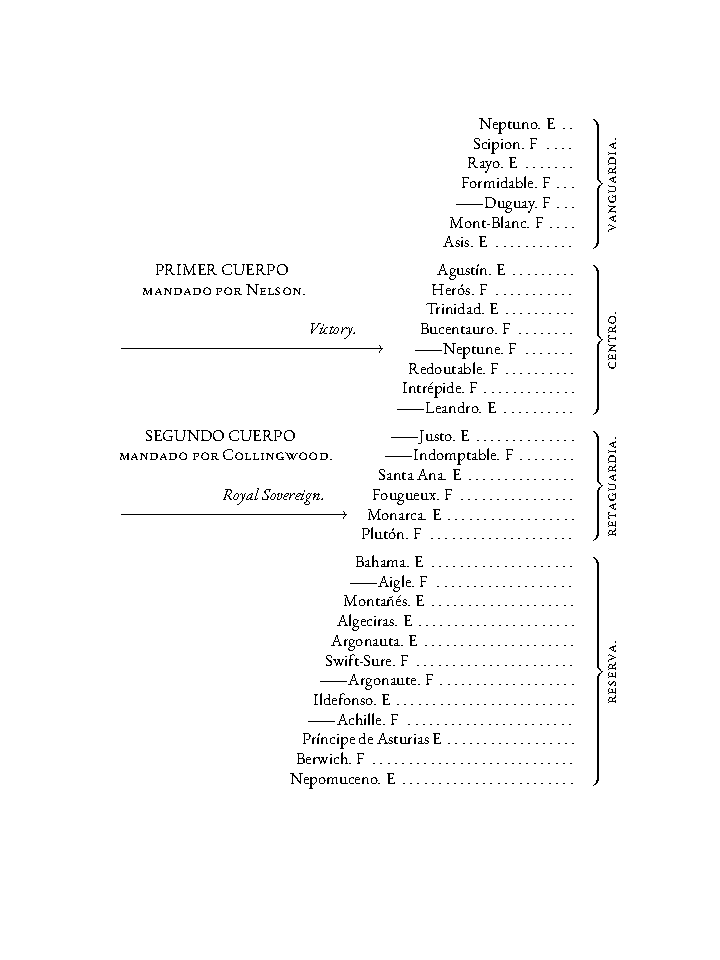
\includepdf{images/trafalgar.pdf}

Eran las doce menos cuarto. El terrible instante se aproximaba. La
ansiedad era general, y no digo esto juzgando por lo que pasaba en mi
espíritu, pues atento a los movimientos del navío en que se decía estaba
Nelson, no pude por un buen rato darme cuenta de lo que pasaba a mi
alrededor.

De repente nuestro comandante dio una orden terrible. La repitieron los
contramaestres. Los marineros corrieron hacia los cabos, chillaron los
motones, trapearon las gavias.

---¡En facha, en facha!---exclamó Marcial, lanzando con energía un
juramento.---Ese condenado se nos quiere meter por la popa.

Al punto comprendí que se había mandado detener la marcha del
\emph{Trinidad} para estrecharle contra el \emph{Bucentauro}, que venía
detrás, porque el \emph{Victory} parecía venir dispuesto a cortar la
línea por entre los dos navíos.

Al ver la maniobra de nuestro buque, pude observar que gran parte de la
tripulación no tenía toda aquella desenvoltura propia de los marineros,
familiarizados como Marcial con la guerra y con la tempestad. Entre los
soldados vi algunos que sentían el malestar del mareo, y se agarraban a
los obenques para no caer. Verdad es que había gente muy decidida,
especialmente en la clase de voluntarios; pero por lo común todos eran
de leva, obedecían las órdenes como de mala gana, y estoy seguro de que
no tenían ni el más leve sentimiento de patriotismo. No les hizo dignos
del combate más que el combate mismo, como advertí después. A pesar del
distinto temple moral de aquellos hombres, creo que en los solemnes
momentos que precedieron al primer cañonazo, la idea de Dios estaba en
todas las cabezas.

Por lo que a mí toca, en toda la vida ha experimentado mi alma
sensaciones iguales a las de aquel momento. A pesar de mis pocos años,
me hallaba en disposición de comprender la gravedad del suceso, y por
primera vez, después que existía, altas concepciones, elevadas imágenes
y generosos pensamientos ocuparon mi mente. La persuasión de la victoria
estaba tan arraigada en mi ánimo, que me inspiraban cierta lástima los
ingleses, y les admiraba al verles buscar con tanto afán una muerte
segura.

Por primera vez entonces percibí con completa claridad la idea de la
patria, y mi corazón respondió a ella con espontáneos sentimientos,
nuevos hasta aquel momento en mi alma. Hasta entonces la patria se me
representaba en las personas que gobernaban la nación, tales como el Rey
y su célebre Ministro, a quienes no consideraba con igual respeto. Como
yo no sabía más historia que la que aprendí en la Caleta, para mí era de
ley que debía uno entusiasmarse al oír que los españoles habían matado
muchos moros primero, y gran pacotilla de ingleses y franceses después.
Me representaba, pues, a mi país como muy valiente; pero el valor que yo
concebía era tan parecido a la barbarie como un huevo a otro huevo. Con
tales pensamientos, el patriotismo no era para mí más que el orgullo de
pertenecer a aquella casta de matadores de moros.

Pero en el momento que precedió al combate, comprendí todo lo que
aquella divina palabra significaba, y la idea de nacionalidad se abrió
paso en mi espíritu, iluminándolo y descubriendo infinitas maravillas,
como el sol que disipa la noche, y saca de la obscuridad un hermoso
paisaje. Me representé a mi país como una inmensa tierra poblada de
gentes, todos fraternalmente unidos; me representé la sociedad dividida
en familias, en las cuales había esposas que mantener, hijos que educar,
hacienda que conservar, honra que defender; me hice cargo de un pacto
establecido entre tantos seres para ayudarse y sostenerse contra un
ataque de fuera, y comprendí que por todos habían sido hechos aquellos
barcos para defender la patria, es decir, el terreno en que ponían sus
plantas, el surco regado con su sudor, la casa donde vivían sus ancianos
padres, el huerto donde jugaban sus hijos, la colonia descubierta y
conquistada por sus ascendientes, el puerto donde amarraban su
embarcación fatigada del largo viaje; el almacén donde depositaban sus
riquezas; la iglesia, sarcófago de sus mayores, habitáculo de sus santos
y arca de sus creencias; la plaza, recinto de sus alegres pasatiempos;
el hogar doméstico, cuyos antiguos muebles, transmitidos de generación
en generación, parecen el símbolo de la perpetuidad de las naciones; la
cocina, en cuyas paredes ahumadas parece que no se extingue nunca el eco
de los cuentos con que las abuelas amansan la travesura e inquietud de
los nietos; la calle, donde se ven desfilar caras amigas; el campo, el
mar, el cielo; todo cuanto desde el nacer se asocia a nuestra
existencia, desde el pesebre de un animal querido hasta el trono de
reyes patriarcales; todos los objetos en que vive prolongándose nuestra
alma, como si el propio cuerpo no le bastara.

Yo creía también que las cuestiones que España tenía con Francia o con
Inglaterra eran siempre porque alguna de estas naciones quería quitarnos
algo, en lo cual no iba del todo descaminado. Parecíame, por tanto, tan
legítima la defensa como brutal la agresión; y como había oído decir que
la justicia triunfaba siempre, no dudaba de la victoria. Mirando
nuestras banderas rojas y amarillas, los colores combinados que mejor
representan al fuego, sentí que mi pecho se ensanchaba; no pude contener
algunas lágrimas de entusiasmo; me acordé de Cádiz, de Vejer; me acordé
de todos los españoles, a quienes consideraba asomados a una gran
azotea, contemplándonos con ansiedad; y todas estas ideas y sensaciones
llevaron finalmente mi espíritu hasta Dios, a quien dirigí una oración
que no era Padre-nuestro ni Ave-María, sino algo nuevo que a mí se me
ocurrió entonces. Un repentino estruendo me sacó de mi arrobamiento,
haciéndome estremecer con violentísima sacudida. Había sonado el primer
cañonazo.

\hypertarget{xi}{%
\chapter{XI}\label{xi}}

Un navío de la retaguardia disparó el primer tiro contra el \emph{Royal
Sovereign}, que mandaba Collingwood. Mientras trababa combate con éste
el \emph{Santa Ana}, el \emph{Victory} se dirigía contra nosotros. En el
\emph{Trinidad} todos demostraban gran ansiedad por comenzar el fuego;
pero nuestro comandante esperaba el momento más favorable. Como si unos
navíos se lo comunicaran a los otros, cual piezas pirotécnicas enlazadas
por una mecha común, el fuego se corrió desde el \emph{Santa Ana} hasta
los dos extremos de la línea.

El \emph{Victory} atacó primero al \emph{Redoutable} francés, y
rechazado por éste, vino a quedar frente a nuestro costado por
barlovento. El momento terrible había llegado; cien voces dijeron
¡\emph{fuego}! repitiendo como un eco infernal la del comandante, y la
andanada lanzó cincuenta proyectiles sobre el navío inglés. Por un
instante el humo me quitó la vista del enemigo. Pero éste, ciego de
coraje, se venía sobre nosotros viento en popa. Al llegar a tiro de
fusil, orzó y nos descargó su andanada. En el tiempo que medió de uno a
otro disparo, la tripulación, que había podido observar el daño hecho al
enemigo, redobló su entusiasmo. Los cañones se servían con presteza,
aunque no sin cierto entorpecimiento, hijo de la poca práctica de
algunos cabos de cañón. Marcial hubiera tomado por su cuenta de buena
gana la empresa de servir una de las piezas de cubierta; pero su cuerpo
mutilado no era capaz de responder al heroísmo de su alma. Se contentaba
con vigilar el servicio de la cartuchería, y con su voz y con su gesto
alentaba a los que servían las piezas.

El \emph{Bucentauro}, que estaba a nuestra popa, hacía fuego igualmente
sobre el \emph{Victory} y el \emph{Temerary}, otro poderoso navío
inglés. Parecía que el navío de Nelson iba a caer en nuestro poder,
porque la artillería del \emph{Trinidad} le había destrozado el aparejo,
y vimos con orgullo que perdía su palo de mesana.

En el ardor de aquel primer encuentro, apenas advertí que algunos de
nuestros marineros caían heridos o muertos. Yo, puesto en el lugar donde
creía estorbar menos, no cesaba de contemplar al comandante, que mandaba
desde el alcázar con serenidad heroica, y me admiraba de ver a mi amo
con menos calma, pero con más entusiasmo, alentando a oficiales y
marineros con su ronca vocecilla.

---¡Ah!---dije yo para mí.---¡Si te viera ahora doña Francisca!

Confesaré que yo tenía momentos de un miedo terrible, en que me hubiera
escondido nada menos que en el mismo fondo de la bodega, y otros de
cierto delirante arrojo en que me arriesgaba a ver desde los sitios de
mayor peligro aquel gran espectáculo. Pero, dejando a un lado mi humilde
persona, voy a narrar el momento más terrible de nuestra lucha con el
\emph{Victory}. El \emph{Trinidad} le destrozaba con mucha fortuna,
cuando el \emph{Temerary}, ejecutando una habilísima maniobra, se
interpuso entre los dos combatientes, salvando a su compañero de
nuestras balas. En seguida se dirigió a cortar la línea por la popa del
\emph{Trinidad}, y como el \emph{Bucentauro}, durante el fuego, se había
estrechado contra éste hasta el punto de tocarse los penoles, resultó un
gran claro, por donde se precipitó el \emph{Temerary}, que viró
prontamente, y colocándose a nuestra aleta de babor, nos disparó por
aquel costado, hasta entonces ileso. Al mismo tiempo, el \emph{Neptune},
otro poderoso navío inglés, colocose donde antes estaba el Victory; éste
se sotaventó, de modo que en un momento el \emph{Trinidad} se encontró
rodeado de enemigos que le acribillaban por todos lados.

En el semblante de mi amo, en la sublime cólera de Uriarte, en los
juramentos de los marineros amigos de Marcial, conocí que estábamos
perdidos, y la idea de la derrota angustió mi alma. La línea de la
escuadra combinada se hallaba rota por varios puntos, y al orden
imperfecto con que se había formado después de la vira en redondo
sucedió el más terrible desorden. Estábamos envueltos por el enemigo,
cuya artillería lanzaba una espantosa lluvia de balas y de metralla
sobre nuestro navío, lo mismo que sobre el \emph{Bucentauro}. El
\emph{Agustín}, el \emph{Heros} y el \emph{Leandro} se batían lejos de
nosotros, en posición algo desahogada, mientras el \emph{Trinidad}, lo
mismo que el navío almirante, sin poder disponer de sus movimientos,
cogidos en terrible escaramuza por el genio del gran Nelson, luchaban
heroicamente, no ya buscando una victoria imposible, sino movidos por el
afán de perecer con honra.

Los cabellos blancos que hoy cubren mi cabeza se erizan todavía al
recordar aquellas tremendas horas, principalmente desde las dos a las
cuatro de la tarde. Se me representan los barcos, no como ciegas
máquinas de guerra, obedientes al hombre, sino como verdaderos gigantes,
seres vivos y monstruosos que luchaban por sí, poniendo en acción, como
ágiles miembros, su velamen, y cual terribles armas, la poderosa
artillería de sus costados. Mirándolos, mi imaginación no podía menos de
personalizarlos, y aun ahora me parece que los veo acercarse,
desafiarse, orzar con ímpetu para descargar su andanada, lanzarse al
abordaje con ademán provocativo, retroceder con ardiente coraje para
tomar más fuerza, mofarse del enemigo, increparle; me parece que les veo
expresar el dolor de la herida, o exhalar noblemente el gemido de la
muerte, como el gladiador que no olvida el decoro de la agonía; me
parece oír el rumor de las tripulaciones, como la voz que sale de un
pecho irritado, a veces alarido de entusiasmo, a veces sordo mugido de
desesperación, precursor de exterminio; ahora himno de júbilo que indica
la victoria; después algazara rabiosa que se pierde en el espacio,
haciendo lugar a un terrible silencio que anuncia la vergüenza de la
derrota.

El espectáculo que ofrecía el interior del \emph{Santísima Trinidad} era
el de un infierno. Las maniobras habían sido abandonadas, porque el
barco no se movía ni podía moverse. Todo el empeño consistía en servir
las piezas con la mayor presteza posible, correspondiendo así al estrago
que hacían los proyectiles enemigos. La metralla inglesa rasgaba el
velamen como si grandes e invisibles uñas le hicieran trizas. Los
pedazos de obra muerta, los trozos de madera, los gruesos obenques
segados cual haces de espigas, los motones que caían, los trozos de
velamen, los hierros, cabos y demás despojos arrancados de su sitio por
el cañón enemigo, llenaban la cubierta, donde apenas había espacio para
moverse. De minuto en minuto caían al suelo o al mar multitud de hombres
llenos de vida; las blasfemias de los combatientes se mezclaban a los
lamentos de los heridos, de tal modo que no era posible distinguir si
insultaban a Dios los que morían, o le llamaban con angustia los que
luchaban.

Yo tuve que prestar auxilio en una faena tristísima, cual era la de
transportar heridos a la bodega, donde estaba la enfermería. Algunos
morían antes de llegar a ella, y otros tenían que sufrir dolorosas
operaciones antes de poder reposar un momento su cuerpo fatigado.
También tuve la indecible satisfacción de ayudar a los carpinteros, que
a toda prisa procuraban aplicar tapones a los agujeros hechos en el
casco; pero por causa de mi poca fuerza, no eran aquellos auxilios tan
eficaces como yo habría deseado.

La sangre corría en abundancia por la cubierta y los puentes, y a pesar
de la arena, el movimiento del buque la llevaba de aquí para allí,
formando fatídicos dibujos. Las balas de cañón, de tan cerca disparadas,
mutilaban horriblemente los cuerpos, y era frecuente ver rodar a alguno,
arrancada a cercén la cabeza, cuando la violencia del proyectil no
arrojaba la víctima al mar, entre cuyas ondas debía perderse casi sin
dolor la última noción de la vida. Otras balas rebotaban contra un palo
o contra la obra muerta, levantando granizada de astillas que herían
como flechas. La fusilería de las cofas y la metralla de las carronadas
esparcían otra muerte menos rápida y más dolorosa, y fue raro el que no
salió marcado más o menos gravemente por el plomo y el hierro de
nuestros enemigos.

De tal suerte combatida y sin poder de ningún modo devolver iguales
destrozos, la tripulación, aquella alma del buque, se sentía perecer,
agonizaba con desesperado coraje, y el navío mismo, aquel cuerpo
glorioso, retemblaba al golpe de las balas. Yo le sentía estremecerse en
la terrible lucha: crujían sus cuadernas, estallaban sus baos,
rechinaban sus puntales a manera de miembros que retuerce el dolor, y la
cubierta trepidaba bajo mis pies con ruidosa palpitación, como si a todo
el inmenso cuerpo del buque se comunicara la indignación y los dolores
de sus tripulantes. En tanto, el agua penetraba por los mil agujeros y
grietas del casco acribillado, y comenzaba a inundar la bodega.

El \emph{Bucentauro}, navío general, se rindió a nuestra vista.
Villeneuve había arriado bandera. Una vez entregado el jefe de la
escuadra, ¿qué esperanza quedaba a los buques? El pabellón francés
desapareció de la popa de aquel gallardo navío, y cesaron sus fuegos. El
\emph{San Agustín} y el \emph{Herós} se sostenían todavía, y el
\emph{Rayo} y el \emph{Neptuno}, pertenecientes a la vanguardia, que
habían venido a auxiliarnos, intentaron en vano salvarnos de los navíos
enemigos que nos asediaban. Yo pude observar la parte del combate más
inmediata al \emph{Santísima Trinidad}, porque del resto de la línea no
era posible ver nada. El viento parecía haberse detenido, y el humo se
quedaba sobre nuestras cabezas, envolviéndonos en su espesa blancura,
que las miradas no podían penetrar. Distinguíamos tan sólo el aparejo de
algunos buques lejanos, aumentados de un modo inexplicable por no sé qué
efecto óptico o porque el pavor de aquel sublime momento agrandaba todos
los objetos.

Disipose por un momento la densa penumbra, ¡pero de qué manera tan
terrible! Detonación espantosa, más fuerte que la de los mil cañones de
la escuadra disparando a un tiempo, paralizó a todos, produciendo
general terror. Cuando el oído recibió tan fuerte impresión, claridad
vivísima había iluminado el ancho espacio ocupado por las dos flotas,
rasgando el velo de humo, y presentose a nuestros ojos todo el panorama
del combate. La terrible explosión había ocurrido hacia el Sur, en el
sitio ocupado antes por la retaguardia.

---Se ha volado un navío,---dijeron todos.

Las opiniones fueron diversas, y se dudaba si el buque volado era el
\emph{Santa Ana}, el \emph{Argonauta}, el \emph{Ildefonso} o el
\emph{Bahama}. Después se supo que había sido el francés nombrado
\emph{Achille}. La expansión de los gases desparramó por mar y cielo en
pedazos mil cuanto momentos antes constituía un hermoso navío con 74
cañones y 600 hombres de tripulación.

Algunos segundos después de la explosión, ya no pensábamos más que en
nosotros mismos.

Rendido el \emph{Bucentauro}, todo el fuego enemigo se dirigió contra
nuestro navío, cuya pérdida era ya segura. El entusiasmo de los primeros
momentos se había apagado en mí, y mi corazón se llenó de un terror que
me paralizaba, ahogando todas las funciones de mi espíritu, excepto la
curiosidad. Ésta era tan irresistible, que me obligó a salir a los
sitios de mayor peligro. De poco servía ya mi escaso auxilio, pues ni
aun se trasladaban los heridos a la bodega, por ser muchos, y las piezas
exigían el servicio de cuantos conservaban un poco de fuerza. Entre
éstos vi a Marcial, que se multiplicaba gritando y moviéndose conforme a
su poca agilidad, y era a la vez contramaestre, marinero, artillero,
carpintero y cuanto había que ser en tan terribles instantes. Nunca creí
que desempeñara funciones correspondientes a tantos hombres el que no
podía considerarse sino como la mitad de un cuerpo humano. Un astillazo
le había herido en la cabeza, y la sangre, tiñéndole la cara, le daba
horrible aspecto. Yo le vi agitar sus labios, bebiendo aquel líquido, y
luego lo escupía con furia fuera del portalón, como si también quisiera
herir a salivazos a nuestros enemigos.

Lo que más me asombraba, causándome cierto espanto, era que Marcial, aun
en aquella escena de desolación, profería frases de buen humor, no sé si
por alentar a sus decaídos compañeros o porque de este modo acostumbraba
alentarse a sí mismo.

Cayó con estruendo el palo de trinquete, ocupando el castillo de proa
con la balumba de su aparejo, y Marcial dijo:

---Muchachos, vengan las hachas. Metamos este mueble en la alcoba.

Al punto se cortaron los cabos, y el mástil cayó al mar.

Y viendo que arreciaba el fuego, gritó dirigiéndose a un pañolero que se
había convertido en cabo de cañón:

---Pero Abad, mándales el vino a esos casacones para que nos dejen en
paz.

Y a un soldado que yacía como muerto, por el dolor de sus heridas y la
angustia del mareo, le dijo aplicándole el botafuego a la nariz:

---Huele una hojita de azahar, camarada, para que se te pase el desmayo.
¿Quieres dar un paseo en bote? Anda; Nelson nos convida a echar unas
cañas.

Esto pasaba en el combés. Alcé la vista al alcázar de popa, y vi que el
general Cisneros había caído. Precipitadamente le bajaron dos marineros
a la cámara. Mi amo continuaba inmóvil en su puesto; pero de su brazo
izquierdo manaba mucha sangre. Corrí hacia él para auxiliarle, y antes
que yo llegase, un oficial se le acercó, intentando convencerle de que
debía bajar a la cámara. No había éste pronunciado dos palabras, cuando
una bala le llevó la mitad de la cabeza, y su sangre salpicó mi rostro.
Entonces, don Alonso se retiró, tan pálido como el cadáver de su amigo,
que yacía mutilado en el piso del alcázar.

Cuando bajó mi amo, el comandante quedó solo arriba, con tal presencia
de ánimo que no pude menos de contemplarle un rato, asombrado de tanto
valor. Con la cabeza descubierta, el rostro pálido, la mirada ardiente,
la acción enérgica, permanecía en su puesto dirigiendo aquella acción
desesperada que no podía ganarse ya. Tan horroroso desastre había de
verificarse con orden, y el comandante era la autoridad que reglamentaba
el heroísmo. Su voz dirigía a la tripulación en aquella contienda del
honor y la muerte.

Un oficial que mandaba en la primera batería subió a tomar órdenes, y
antes de hablar cayó muerto a los pies de su jefe; otro guardia marina
que estaba a su lado cayó también malherido, y Uriarte quedó al fin
enteramente solo en el alcázar, cubierto de muertos y heridos. Ni aun
entonces se apartó su vista de los barcos ingleses ni de los movimientos
de nuestra artillería; y el imponente aspecto del alcázar y toldilla,
donde agonizaban sus amigos y subalternos, no conmovió su pecho varonil
ni quebrantó su enérgica resolución de sostener el fuego hasta perecer.
¡Ah! recordando yo después la serenidad y estoicismo de don Francisco
Javier Uriarte, he podido comprender todo lo que nos cuentan de los
heroicos capitanes de la antigüedad. Entonces no conocía yo la palabra
sublimidad; pero viendo al comandante del \emph{Trinidad} comprendí que
todos los idiomas deben tener un hermoso vocablo para expresar aquella
grandeza de alma que me parecía favor rara vez otorgado por Dios al
hombre miserable.

Entre tanto, gran parte de los cañones había cesado de hacer fuego,
porque la mitad de la gente estaba fuera de combate. Tal vez no me
hubiera fijado en esta circunstancia, si habiendo salido de la cámara,
impulsado por mi curiosidad, no sintiera una voz que con acento terrible
me dijo:---¡Gabrielillo, aquí!

Marcial me llamaba; acudí prontamente, y le hallé empeñado en servir uno
de los cañones que habían quedado sin gente. Una bala había llevado a
Medio-hombre la punta de su pierna de palo, lo cual le hacía decir:

---Si llego a traer la de carne y hueso\ldots{}

Dos marinos muertos yacían a su lado; un tercero, gravemente herido, se
esforzaba en seguir sirviendo la pieza.

---Compadre---le dijo Marcial,---ya tú no puedes ni encender una
colilla.

Arrancó el botafuego de manos del herido y me lo entregó diciendo:

---Toma, Gabrielillo; si tienes miedo, vas al agua.

Esto diciendo, cargó el cañón con toda la prisa que le fue posible,
ayudado de un grumete que estaba casi ileso; lo cebaron y apuntaron;
ambos exclamaron «fuego;» acerqué la mecha, y el cañón disparó.

Se repitió la operación por segunda y tercera vez, y el ruido del cañón,
disparado por mí, retumbó de un modo extraordinario en mi alma. El
considerarme, no ya espectador, sino actor decidido en tan grandiosa
tragedia, disipó por un instante el miedo, y me sentí con grandes bríos,
al menos con la firme resolución de aparentarlos. Desde entonces conocí
que el heroísmo es casi siempre una forma del pundonor. Marcial y otros
me miraban; era preciso que me hiciera digno de fijar su atención.

«¡Ah!---decía yo para mí con orgullo.---Si mi amita pudiera verme
ahora\ldots{} ¡Qué valiente estoy disparando cañonazos como un
hombre!\ldots{} Lo menos habré mandado al otro mundo dos docenas de
ingleses.»

Pero estos nobles pensamientos me ocuparon muy poco tiempo, porque
Marcial, cuya fatigada naturaleza comenzaba a rendirse después de su
esfuerzo, respiro con ansia, se secó la sangre que afluía en abundancia
de su cabeza, cerró los ojos, sus brazos se extendieron con desmayo, y
dijo:

---No puedo más; se me sube la pólvora a la toldilla (la cabeza).
Gabriel, tráeme agua.

Corrí a buscar el agua, y cuando se la traje, bebió con ansia. Pareció
tomar con esto nuevas fuerzas. Íbamos a seguir, cuando un gran estrépito
nos dejó sin movimiento. El palo mayor, tronchado por la fogonadura,
cayo sobre el combés, y tras él el de mesana. El navío quedó lleno de
escombros y el desorden fue espantoso.

Felizmente quedé en hueco y sin recibir más que una ligera herida en la
cabeza, la cual, aunque me aturdió al principio, no me impidió apartar
los trozos de vela y cabos que habían caído sobre mí. Los marineros y
soldados de cubierta pugnaban por desalojar tan enorme masa de cuerpos
inútiles, y desde entonces sólo la artillería de las baterías bajas
sostuvo el fuego. Salí como pude, busqué a Marcial, no le hallé, y
habiendo fijado mis ojos en el alcázar, noté que el comandante ya no
estaba allí. Gravemente herido de un astillazo en la cabeza, había caído
exánime, y al punto dos marineros subieron para trasladarle a la cámara.
Corrí también allá, y entonces un casco de metralla me hirió en el
hombro, lo que me asustó en extremo, creyendo que mi herida era mortal y
que iba a exhalar el último suspiro. Mi turbación no me impidió entrar
en la cámara, donde por la mucha sangre que brotaba de mi herida me
debilité, quedando por un momento desvanecido.

En aquel pasajero letargo, seguí oyendo el estrépito de los cañones de
la segunda y tercera batería, y después una voz que decía con furia:

---¡Abordaje!\ldots{} ¡las picas!\ldots{} ¡las hachas!

Después la confusión fue tan grande, que no pude distinguir lo que
pertenecía a las voces humanas en tal descomunal concierto. Pero no sé
cómo, sin salir de aquel estado de somnolencia, me hice cargo de que se
creía todo perdido, y de que los oficiales se hallaban reunidos en la
cámara para acordar la rendición; y también puedo asegurar que si no fue
invento de mi fantasía, entonces trastornada, resonó en el combés una
voz que decía: «¡El \emph{Trinidad} no se rinde!.» De fijo fue la voz de
Marcial, si es que realmente dijo alguien tal cosa.

Me sentí despertar, y vi a mi amo arrojado sobre uno de los sofás de la
cámara, con la cabeza oculta entre las manos en ademán de desesperación
y sin cuidarse de su herida.

Acerqueme a él, y el infeliz anciano no halló mejor modo de expresar su
desconsuelo que abrazándome paternalmente, como si ambos estuviéramos
cercanos a la muerte. Él, por lo menos, creo que se consideraba próximo
a morir de puro dolor, porque su herida no tenía la menor gravedad. Yo
le consolé como pude, diciendo que si la acción no se había ganado, no
fue porque yo dejara de matar bastante ingleses con mi cañoncito, y
añadí que para otra vez seríamos más afortunados; pueriles razones que
no calmaron su agitación.

Saliendo afuera en busca de agua para mi amo, presencié el acto de
arriar la bandera, que aún flotaba en la cangreja, uno de los pocos
restos de arboladura que con el tronco de mesana quedaban en pie. Aquel
lienzo glorioso, ya agujereado por mil partes, señal de nuestra honra,
que congregaba bajo sus pliegues a todos los combatientes, descendió del
mástil para no izarse más. La idea de un orgullo abatido, de un ánimo
esforzado que sucumbe ante fuerzas superiores, no puede encontrar imagen
más perfecta para representarse a los ojos humanos que la de aquella
oriflama que se abate y desaparece como un sol que se pone. El de
aquella tarde tristísima, tocando al término de su carrera en el momento
de nuestra rendición, iluminó nuestra bandera con su último rayo.

El fuego cesó y los ingleses penetraron en el barco vencido.

\hypertarget{xii}{%
\chapter{XII}\label{xii}}

Cuando el espíritu, reposando de la agitación del combate, tuvo tiempo
de dar paso a la compasión, al frío terror producido por la vista de tan
grande estrago, se presentó a los ojos de cuantos quedamos vivos la
escena del navío en toda su horrenda majestad. Hasta entonces los ánimos
no se habían ocupado más que de la defensa; mas cuando el fuego cesó, se
pudo advertir el gran destrozo del casco, que, dando entrada al agua por
sus mil averías, se hundía, amenazando sepultarnos a todos, vivos y
muertos, en el fondo del mar. Apenas entraron en él los ingleses, un
grito resonó unánime, proferido por nuestros marinos:

---¡A las bombas!

Todos los que podíamos acudimos a ellas y trabajamos con ardor; pero
aquellas máquinas imperfectas desalojaban una cantidad de agua bastante
menor que la que entraba. De repente un grito, aún más terrible que el
anterior, nos llenó de espanto. Ya dije que los heridos se habían
transportado al último sollado, lugar que, por hallarse bajo la línea de
flotación, está libre de la acción de las balas. El agua invadía
rápidamente aquel recinto, y algunos marinos asomaron por la escotilla
gritando:

---¡Que se ahogan los heridos!

La mayor parte de la tripulación vaciló entre seguir desalojando el agua
y acudir en socorro de aquellos desgraciados; y no sé qué habría sido de
ellos, si la gente de un navío inglés no hubiera acudido en nuestro
auxilio. Éstos no sólo transportaron los heridos a la tercera y a la
segunda batería, sino que también pusieron mano a las bombas, mientras
sus carpinteros trataban de reparar algunas de las averías del casco.

Rendido de cansancio, y juzgando que don Alonso podía necesitar de mí,
fui a la cámara. Entonces vi a algunos ingleses ocupados en poner el
pabellón británico en la popa del Santísima Trinidad. Como cuento con
que el lector benévolo me ha de perdonar que apunte aquí mis
impresiones, diré que aquello me hizo pensar un poco. Siempre se me
habían representado los ingleses como verdaderos piratas o salteadores
de los mares, gentezuela aventurera que no constituía nación y que vivía
del merodeo. Cuando vi el orgullo con que enarbolaron su pabellón,
saludándole con vivas aclamaciones; cuando advertí el gozo y la
satisfacción que les causaba haber apresado el más grande y glorioso
barco que hasta entonces surcó los mares, pensé que también ellos
tendrían su patria querida, que ésta les habría confiado la defensa de
su honor; me pareció que en aquella tierra, para mí misteriosa, que se
llamaba Inglaterra, habían de existir, como en España, muchas gentes
honradas, un rey paternal, y las madres, las hijas, las esposas, las
hermanas de tan valientes marinos, los cuales, esperando con ansiedad su
vuelta, rogarían a Dios que les concediera la victoria.

En la cámara encontré a mi señor más tranquilo. Los oficiales ingleses
que habían entrado allí trataban a los nuestros con delicada cortesía, y
según entendí, querían trasbordar los heridos a algún barco enemigo. Uno
de aquellos oficiales se acercó a mi amo como queriendo reconocerle, y
le saludó en español medianamente correcto, recordándole una amistad
antigua. Contestó don Alonso a sus finuras con gravedad, y después quiso
enterarse por él de los pormenores del combate.

---¿Pero qué ha sido de la reserva? ¿Qué ha hecho Gravina?---preguntó mi
amo.

---Gravina se ha retirado con algunos navíos---contestó el inglés.

---De la vanguardia sólo han venido a auxiliarnos el \emph{Rayo} y el
\emph{Neptuno}.

---Los cuatro franceses, \emph{Duguay-Trouin}, \emph{Mont-Blanc},
\emph{Scipion} y \emph{Formidable}, son los únicos que no han entrado en
acción.

---Pero Gravina, Gravina, ¿qué es de Gravina?---insistió mi amo.

---Se ha retirado en el \emph{Príncipe de Asturias}; mas como se le ha
dado caza, ignoro si habrá llegado a Cádiz.

---¿Y el \emph{San Ildefonso}?

---Ha sido apresado.

---¿Y el \emph{Santa Ana}?

---También ha sido apresado.

---¡Vive Dios!---exclamó don Alonso sin poder disimular su
enojo.---Apuesto a que no ha sido apresado el \emph{Nepomuceno}.

---También lo ha sido.

---¡Oh! ¿está usted seguro de ello? ¿Y Churruca?

---Ha muerto---contestó el inglés con tristeza.

---¡Oh! ¡Ha muerto! ¡Ha muerto Churruca!---exclamó mi amo con angustiosa
perplejidad.---Pero el \emph{Bahama} se habrá salvado, el \emph{Bahama}
habrá vuelto ileso a Cádiz.

---También ha sido apresado.

---¡También! ¿Y Galiano? Galiano es un héroe y un sabio.

---Sí---repuso sombríamente el inglés;---pero ha muerto también.

---¿Y qué es del \emph{Montañés}? ¿Qué ha sido de Alcedo?

---Alcedo\ldots{} también ha muerto.

Mi amo no pudo reprimir la expresión de su profunda pena; y como la
avanzada edad amenguaba en él la presencia de ánimo propia de tan
terribles momentos, hubo de pasar por la pequeña mengua de derramar
algunas lágrimas, triste obsequio a sus compañeros. No es impropio el
llanto en las grandes almas; antes bien, indica el consorcio fecundo de
la delicadeza de sentimientos con la energía de carácter. Mi amo lloró
como hombre, después de haber cumplido con su deber como marino; mas
reponiéndose de aquel abatimiento, y buscando alguna razón con que
devolver al inglés la pesadumbre que éste le causara, dijo:

---Pero ustedes no habrán sufrido menos que nosotros. Nuestros enemigos
habrán tenido pérdidas de consideración.

---Una sobre todo irreparable---contestó el inglés con tanta congoja
como la de don Alonso.---Hemos perdido al primero de nuestros marinos,
al valiente entre los valientes, al heroico, al divino, al sublime
almirante Nelson.

Y con tan poca entereza como mi amo, el oficial inglés no se cuidó de
disimular su inmensa pena: cubriose la cara con las manos y lloró, con
toda la expresiva franqueza del verdadero dolor, al jefe, al protector y
al amigo.

Nelson, herido mortalmente en mitad del combate, según después supe, por
una bala de fusil que le atravesó el pecho y se fijó en la espina
dorsal, dijo al capitán Hardy:---Se acabó; al fin lo han conseguido. Su
agonía se prolongó hasta el caer de la tarde; no perdió ninguno de los
pormenores del combate, ni se extinguió su genio de militar y de marino
sino cuando la última fugitiva palpitación de la vida se disipó en su
cuerpo herido. Atormentado por horribles dolores, no dejó de dictar
órdenes, enterándose de los movimientos de ambas escuadras, y cuando se
le hizo saber el triunfo de la suya, exclamó:---Bendito sea Dios; he
cumplido con mi deber.

Un cuarto de hora después expiraba el primer marino de nuestro siglo.

Perdóneseme la digresión. El lector extrañará que no conociéramos la
suerte de muchos buques de la escuadra combinada. Nada más natural que
nuestra ignorancia, por causa de la desmesurada longitud de la línea de
combate, y además el sistema de luchas parciales adoptado por los
ingleses. Sus navíos se habían mezclado con los nuestros, y como la
contienda era a tiro de fusil, el buque enemigo que nos batía ocultaba
la vista del resto de la escuadra, además de que el humo espesísimo nos
impedía ver cuanto no se hallara en paraje cercano.

Al anochecer, y cuando aún el cañoneo no había cesado, distinguíamos
algunos navíos, que pasaban a un largo como fantasmas, unos con media
arboladura, otros completamente desarbolados. La bruma, el humo, el
mismo aturdimiento de nuestras cabezas, nos impedía distinguir si eran
españoles o enemigos; y cuando la luz de un fogonazo lejano iluminaba a
trechos aquel panorama temeroso, notábamos que aún seguía la lucha con
encarnizamiento entre grupos de navíos aislados; que otros corrían sin
concierto ni rumbo, llevados por el temporal, y que alguno de los
nuestros era remolcado por otro inglés en dirección al Sur.

Vino la noche, y con ella aumentó la gravedad y el horror de nuestra
situación. Parecía que la Naturaleza había de sernos propicia después de
tantas desgracias; pero, por el contrario, desencadenáronse con furia
los elementos, como si el Cielo creyera que aún no era bastante grande
el número de nuestras desdichas. Desatose un recio temporal, y viento y
agua, hondamente agitados, azotaron el buque, que, incapaz de maniobra,
fluctuaba a merced de las olas. Los vaivenes eran tan fuertes que se
hacía difícil el trabajo, lo cual, unido al cansancio de la tripulación,
empeoraba nuestro estado de hora en hora. Un navío inglés, que después
supe se llamaba \emph{Prince}, trató de remolcar al Trinidad; pero sus
esfuerzos fueron inútiles, y tuvo que alejarse por temor a un choque,
que habría sido funesto para ambos buques.

Entre tanto no era posible tomar alimento alguno, y yo me moría de
hambre, porque los demás, indiferentes a todo lo que no fuera el
peligro, apenas se cuidaban de cosa tan importante. No me atrevía a
pedir un pedazo de pan por temor de parecer importuno, y al mismo
tiempo, sin vergüenza lo confieso, dirigía mi escrutadora observación a
todos los sitios donde colegía que podían existir provisiones de boca.
Apretado por la necesidad, me arriesgué a hacer una visita a los pañoles
del bizcocho, y ¿cuál sería mi asombro cuando vi que Marcial estaba
allí, trasegando a su estómago lo primero que encontró a mano? El
anciano estaba herido de poca gravedad, y aunque una bala le había
llevado el pie derecho, como este no era otra cosa que la extremidad de
la pierna de palo, el cuerpo de Marcial sólo estaba con tal percance un
poco más cojo.

---Toma, Gabrielillo---me dijo, llenándome el seno de galletas;---barco
sin lastre no navega.

En seguida empinó una botella y bebió con delicia.

Salimos del pañol, y vi que no éramos nosotros solos los que visitaban
aquel lugar, pues todo indicaba que un desordenado pillaje había
ocurrido allí momentos antes.

Reparadas mis fuerzas, pude pensar en servir de algo, poniendo mano a
las bombas o ayudando a los carpinteros. Trabajosamente se enmendaron
algunas averías con auxilio de los ingleses, que vigilaban todo, y según
después comprendí, no perdían de vista a algunos de nuestros marineros,
porque temían que se sublevasen, represando el navío, en lo cual los
enemigos demostraban más suspicacia que buen sentido, pues menester era
haber perdido el juicio para intentar represar un buque en tal estado.
Ello es que los \emph{casacones} acudían a todas partes y no perdían
movimiento alguno.

Entrada la noche, y hallándome transido de frío, abandoné la cubierta,
donde apenas podía tenerme, y corría además el peligro de ser arrebatado
por un golpe de mar, y me retiré a la cámara. Mi primera intención fue
dormir un poco; pero ¿quién dormía en aquella noche?

En la cámara todo era confusión, lo mismo que en el combés. Los sanos
asistían a los heridos, y éstos, molestados a la vez por sus dolores y
por el movimiento del buque, que les impedía todo reposo, ofrecían tan
triste aspecto, que a su vista era imposible entregarse al descanso. En
un lado de la cámara yacían, cubiertos con el pabellón nacional, los
oficiales muertos. Entre tanta desolación, ante el espectáculo de tantos
dolores, había en aquellos cadáveres no sé qué de envidiable: ellos
solos descansaban a bordo del \emph{Trinidad}, y todo les era ajeno,
fatigas y penas, la vergüenza de la derrota y los padecimientos físicos.
La bandera que les servía de ilustre mortaja parecía ponerles fuera de
aquella esfera de responsabilidad, de mengua y desesperación en que
todos nos encontrábamos. Nada les afectaba el peligro que corría la
nave, porque ésta no era ya más que su ataúd.

Los oficiales muertos eran: don Juan Cisniega, teniente de navío, el
cual no tenía parentesco con mi amo a pesar de la identidad de apellido;
don Joaquín de Salas y don Juan Matute, también tenientes de navío; el
teniente coronel de ejército don José Graullé, el teniente de fragata
Urías y el guardia marina don Antonio de Bobadilla. Los marineros y
soldados muertos, cuyos cadáveres yacían sin orden en las baterías y
sobre cubierta, ascendían a la terrible suma de cuatrocientos.

No olvidaré jamás el momento en que aquellos cuerpos fueron arrojados al
mar por orden del oficial inglés que custodiaba el navío. Verificose la
triste ceremonia al amanecer del día 22, hora en que el temporal parece
que arreció ex profeso, para aumentar la pavura de semejante escena.
Sacados sobre cubierta los cuerpos de los oficiales, el cura rezó un
responso a toda prisa, porque no era ocasión de andarse en dibujos, e
inmediatamente se procedió al acto solemne. Envueltos en su bandera, y
con una bala atada a los pies, fueron arrojados al mar, sin que esto,
que ordinariamente hubiera producido en todos tristeza y consternación,
conmoviera entonces a los que lo presenciaron. ¡Tan hechos estaban los
ánimos a la desgracia, que el espectáculo de la muerte les era poco
menos que indiferente! Las exequias del mar son más tristes que las de
la tierra. Se da sepultura a un cadáver, y allí queda; las personas a
quienes interesa saben que hay un rincón de tierra donde existen
aquellos restos, y pueden marcarlos con una losa, con una cruz o con una
piedra. Pero en el mar\ldots{} se arrojan los cuerpos en la movible
inmensidad, y parece que dejan de existir en el momento de caer; la
imaginación no puede seguirlos en su viaje al profundo abismo, y es
difícil suponer que estén en alguna parte estando en el fondo del
Océano. Estas reflexiones hacía yo viendo cómo desaparecían los cuerpos
de aquellos ilustres guerreros, un día antes llenos de vida, gloria de
su patria y encanto de sus familias.

Los marineros muertos eran arrojados con menos ceremonia: la Ordenanza
manda que se les envuelva en el coy; pero en aquella ocasión no había
tiempo para entretenerse en cumplir la Ordenanza. A algunos se les
amortajó como está mandado; pero la mayor parte fueron echados al mar
sin ningún atavío y sin bala a los pies, por la sencilla razón de que no
había para todos. Eran cuatrocientos, próximamente, y a fin de terminar
pronto la operación de darles sepultura, fue preciso que pusieran mano a
la obra todos los hombres útiles que a bordo había para despachar más
pronto. Muy a disgusto mío tuve que ofrecer mi cooperación para tan
triste servicio, y algunos cuerpos cayeron al mar soltados desde la
borda por mi mano, puesta en ayuda de otras más vigorosas.

Entonces ocurrió un hecho, una coincidencia que me causó mucho terror.
Un cadáver horriblemente desfigurado, fue cogido entre dos marineros, y
en el momento de levantarlo en alto, algunos de los circunstantes se
permitieron groseras burlas, que en toda ocasión habrían sido
importunas, y en aquel momento infames. No sé por qué el cuerpo de aquel
desgraciado fue el único que les movió a perder con tal descaro el
respeto a la muerte, y decían: «Ya las ha pagado todas juntas\ldots; no
volverá a hacer de las suyas,» y otras groserías del mismo jaez. Aquello
me indignó; pero mi indignación se trocó en asombro y en un sentimiento
indefinible, mezcla de respeto, de pena y de miedo, cuando observando
atentamente las facciones mutiladas de aquel cadáver, reconocí en él a
mi tío\ldots{} Cerré los ojos con espanto, y no los abrí hasta que el
violento salpicar del agua me indicó que había desaparecido para siempre
ante la vista humana.

Aquel hombre había sido muy malo para mí, muy malo para su hermana; pero
era mi pariente cercano, hermano de mi madre; la sangre que corría por
mis venas era su sangre, y esa voz interna que nos incita a ser
benévolos con las faltas de los nuestros, no podía permanecer callada
después de la escena que pasó ante mis ojos. Al mismo tiempo, yo había
podido reconocer en la cara ensangrentada de mi tío algunos rasgos
fisonómicos de la cara de mi madre, y esto aumentó mi aflicción. En
aquel momento no me acordé de que había sido un gran criminal, ni menos
de las crueldades que usó conmigo durante mi infortunada niñez. Yo les
aseguro a ustedes, y no dudo en decir esto, aunque sea en elogio mío,
que le perdoné con toda mi alma y que elevé el pensamiento a Dios,
pidiéndole que le perdonara todas sus culpas.

Después supe que se había portado heroicamente en el combate, sin que
por esto alcanzara las simpatías de sus compañeros, quienes, reputándole
como el más bellaco de los hombres, no tuvieron para él una palabra de
afecto o conmiseración, ni aun en el momento supremo en que toda falta
se perdona, porque se supone al criminal dando cuenta de sus actos ante
Dios.

Avanzado el día, intentó de nuevo el navío \emph{Prince} remolcar al
\emph{Santísima Trinidad}; pero con tan poca fortuna como en la noche
anterior. La situación no empeoraba, a pesar de que seguía el temporal
con igual fuerza, pues se habían reparado muchas averías, y se creía
que, una vez calmado el tiempo, podría salvarse el casco. Los ingleses
tenían gran empeño en ello, porque querían llevar por trofeo a Gibraltar
el más grande navío hasta entonces construido. Por esta razón trabajaban
con tanto ahínco en las bombas noche y día, permitiéndonos descansar
algún rato.

Durante todo el día 22 la mar se revolvía con frenesí, llevando y
trayendo el casco del navío cual si fuera endeble lancha de pescadores;
y aquella montaña de madera probaba la fuerte trabazón de sus sólidas
cuadernas, cuando no se rompía en mil pedazos al recibir el tremendo
golpear de las olas. Había momentos en que, aplanándose el mar, parecía
que el navío iba a hundirse para siempre; pero inflamándose la ola como
al impulso de profundo torbellino, levantaba aquél su orgullosa proa,
adornada con el león de Castilla, y entonces respirábamos con la
esperanza de salvarnos.

Por todos lados descubríamos navíos dispersos, la mayor parte ingleses,
no sin grandes averías y procurando todos alcanzar la costa para
refugiarse. También los vimos españoles y franceses, unos desarbolados,
otros remolcados por algún barco enemigo. Marcial reconoció en uno de
éstos al \emph{San Ildefonso}. Vimos flotando en el agua multitud de
restos y despojos, como masteleros, cofas, lanchas rotas, escotillas,
trozos de balconaje, portas, y, por último, avistamos dos infelices
marinos que, mal embarcados en un gran palo, eran llevados por las olas,
y habrían perecido si los ingleses no corrieran al instante a darles
auxilio. Traídos a bordo del \emph{Trinidad}, volvieron a la vida, que,
recobrada después de sentirse en los brazos de la muerte, equivale a
nacer de nuevo.

El día pasó entre agonías y esperanzas; ya nos parecía que era
indispensable el trasbordo a un buque inglés para salvarnos, ya creíamos
posible conservar el nuestro. De todos modos, la idea de ser llevados a
Gibraltar como prisioneros era terrible, si no para mí, para los hombres
pundonorosos y obstinados como mi amo, cuyos padecimientos morales
debieron de ser inauditos aquel día. Pero estas dolorosas alternativas
cesaron por la tarde, y a la hora en que fue unánime la idea de que si
no trasbordábamos pereceríamos todos en el buque, que ya tenía quince
pies de agua en la bodega. Iriartea y Cisneros recibieron aquella
noticia con calma y serenidad, demostrando que no hallaban gran
diferencia entre morir en la casa propia o ser prisioneros en la
extraña. Acto continuo comenzó el trasbordo a la escasa luz del
crepúsculo, lo cual no era cosa fácil, habiendo precisión de embarcar
cerca de trescientos heridos. La tripulación sana constaba de unos
quinientos hombres, cifra a que quedaron reducidos los mil ciento quince
individuos de que se componía antes del combate.

Comenzó precipitadamente el trasbordo con las lanchas del
\emph{Trinidad}, las del \emph{Prince} y las de otros tres buques de la
escuadra inglesa. Diose la preferencia a los heridos; mas aunque se
trató de evitarles toda molestia, fue imposible levantarles de donde
estaban sin mortificarles, y algunos pedían con fuertes gritos que los
dejasen tranquilos, prefiriendo la muerte a un viaje que recrudecía sus
dolores. La premura no daba lugar a la compasión, y eran conducidos a
las lanchas tan sin piedad como arrojados al mar fueron los fríos
cadáveres de sus compañeros.

El comandante Iriartea y el jefe de escuadra, Cisneros se embarcaron en
los botes de la oficialidad inglesa; y habiendo instado a mi amo para
que entrase también en ellos, éste se negó resueltamente, diciendo que
deseaba ser el último en abandonar el \emph{Trinidad}. Esto no dejó de
contrariarme, porque desvanecidos en mí los efluvios de patriotismo, que
al principio me dieron cierto arrojo, no pensaba ya más que en salvar mi
vida, y no era lo más a propósito para este noble fin el permanecer a
bordo de un buque que se hundía por momentos.

Mis temores no fueron vanos, pues aún no estaba fuera la mitad de la
tripulación cuando un sordo rumor de alarma y pavor resonó en nuestro
navío.

---¡Que nos vamos a pique!\ldots{} ¡a las lanchas, a las
lanchas!---exclamaron algunos, mientras dominados todos por el instinto
de conservación, corrían hacia la borda, buscando con ávidos ojos las
lanchas que volvían. Se abandonó todo trabajo; no se pensó más en los
heridos, y muchos de éstos, sacados ya sobre cubierta, se arrastraban
por ella con delirante extravío, buscando un portalón por donde
arrojarse al mar. Por las escotillas salía un lastimero clamor, que aún
parece resonar en mi cerebro, helando la sangre en mis venas y erizando
mis cabellos. Eran los heridos que quedaban en la primera batería, los
cuales, sintiéndose anegados por el agua, que ya invadía aquel sitio,
clamaban pidiendo socorro no sé si a Dios o a los hombres.

A éstos se lo pedían en vano, porque no pensaban sino en la propia
salvación. Se arrojaron precipitadamente a las lanchas, y esta confusión
en la lobreguez de la noche, entorpecía el trasbordo. Un solo hombre,
impasible ante tan gran peligro, permanecía en el alcázar sin atender a
lo que pasaba a su alrededor, y se paseaba preocupado y meditabundo,
como si aquellas tablas donde ponía su pie no estuvieran solicitadas por
el inmenso abismo. Era mi amo.

Corrí hacia él despavorido, y le dije:

---¡Señor, que nos ahogamos!

Don Alonso no me hizo caso, y aun creo, si la memoria no me es infiel,
que sin abandonar su actitud pronunció palabras tan ajenas a la
situación como éstas:

---¡Oh! Cómo se va a reír Paca cuando yo vuelva a casa después de esta
gran derrota.

---¡Señor, que el barco se va a pique!---exclamé de nuevo, no ya
pintando el peligro, sino suplicando con gestos y voces.

Mi amo miró al mar, a las lanchas, a los hombres que, desesperados y
ciegos, se lanzaban a ellas; y yo busqué con ansiosos ojos a Marcial, y
le llamé con toda la fuerza de mis pulmones. Entonces paréceme que perdí
la sensación de lo que ocurría, me aturdí, se nublaron mis ojos y no sé
lo que pasó. Para contar cómo me salvé, no puedo fundarme sino en
recuerdos muy vagos, semejantes a las imágenes de un sueño, pues sin
duda el terror me quitó el conocimiento. Me parece que un marinero se
acercó a don Alonso cuando yo le hablaba, y le asió con sus vigorosos
brazos. Yo mismo me sentí transportado, y cuando mi nublado espíritu se
aclaró un poco, me vi en una lancha, recostado sobre las rodillas de mi
amo, el cual tenía mi cabeza entre sus manos con paternal cariño.
Marcial empuñaba la caña del timón; la lancha estaba llena de gente.

Alcé la vista y vi como a cuatro o cinco varas de distancia, a mi
derecha, el negro costado del navío, próximo a hundirse; por los
portalones a que aún no había llegado el agua, salía una débil claridad,
la de la lámpara encendida al anochecer, y que aún velaba, guardián
incansable, sobre los restos del buque abandonado. También hirieron mis
oídos algunos lamentos que salían por las troneras: eran los pobres
heridos que no había sido posible salvar y se hallaban suspendidos sobre
el abismo, mientras aquella triste luz les permitía mirarse,
comunicándose con los ojos la angustia de los corazones.

Mi imaginación se trasladó de nuevo al interior del buque; una pulgada
de agua faltaba no más para romper el endeble equilibrio que aún le
sostenía. ¡Cómo presenciarían aquellos infelices el crecimiento de la
inundación! ¡Qué dirían en aquel momento terrible! Y si vieron a los que
huían en las lanchas, si sintieron el chasquido de los remos, ¡con
cuánta amargura gemirían sus almas atribuladas! Pero también es cierto
que aquel atroz martirio las purificó de toda culpa, y que la
misericordia de Dios llenó todo el ámbito del navío en el momento de
sumergirse para siempre.

La lancha se alejó; yo seguí viendo aquella gran masa informe, aunque
sospecho que era mi fantasía, no mis ojos, la que miraba el Trinidad en
la obscuridad de la noche, y hasta creí distinguir en el negro cielo un
gran brazo que descendía hasta la superficie de las aguas. Fue sin duda
la imagen de mis pensamientos reproducida por los sentidos.

\hypertarget{xiii}{%
\chapter{XIII}\label{xiii}}

La lancha se dirigió\ldots{} ¿a dónde? Ni el mismo Marcial sabía a dónde
nos dirigíamos. La obscuridad era tan fuerte, que perdimos de vista las
demás lanchas, y las luces del navío Prince se desvanecieron tras la
niebla, como si un soplo las hubiera extinguido. Las olas eran tan
gruesas, y el vendaval tan recio, que la débil embarcación avanzaba muy
poco, y gracias a una hábil dirección no zozobró más de una vez. Todos
callábamos, y los más fijaban una triste mirada en el sitio donde se
suponía que nuestros compañeros abandonados luchaban en aquel instante
con la muerte en espantosa agonía.

No acabó aquella travesía sin hacer, conforme a mi costumbre, algunas
reflexiones, que bien puedo aventurarme a llamar filosóficas. Alguien se
reirá de un filósofo de catorce años; pero yo no me turbaré ante las
burlas, y tendré el atrevimiento de escribir aquí mis reflexiones de
entonces. Los niños también suelen pensar grandes cosas; y en aquella
ocasión, ante aquel espectáculo, ¿qué cerebro, como no fuera el de un
idiota, podría permanecer en calma?

Pues bien: en nuestras lanchas iban españoles e ingleses, aunque era
mayor el número de los primeros, y era curioso observar cómo
fraternizaban, amparándose unos a otros en el común peligro, sin
recordar que el día anterior se mataban en horrenda lucha, más parecidos
a fieras que a hombres. Yo miraba a los ingleses, remando con tanta
decisión como los nuestros; yo observaba en sus semblantes las mismas
señales de terror o de esperanza, y, sobre todo, la expresión propia del
santo sentimiento de humanidad y caridad, que era el móvil de unos y
otros. Con estos pensamientos, decía para mí: «¿Para qué son las
guerras, Dios mío? ¿Por qué estos hombres no han de ser amigos en todas
las ocasiones de la vida como lo son en las de peligro? Esto que veo,
¿no prueba que todos los hombres son hermanos?.»

Pero venía de improviso a cortar estas consideraciones, la idea de
nacionalidad, aquel sistema de islas que yo había forjado, y entonces
decía: ---Pero ya; esto de que las islas han de querer quitarse unas a
otras algún pedazo de tierra, lo echa todo a perder, y sin duda en todas
ellas debe de haber hombres muy malos, que son los que arman las guerras
para su provecho particular, bien porque son ambiciosos y quieren
mandar, bien porque son avaros y anhelan ser ricos. Estos hombres malos
son los que engañan a los demás, a todos estos infelices que van a
pelear; y para que el engaño sea completo, les impulsan a odiar a otras
naciones; siembran la discordia, fomentan la envidia, y aquí tienen
ustedes el resultado. Yo estoy seguro---añadí,---de que esto no puede
durar; apuesto doble contra sencillo a que dentro de poco los hombres de
unas y otras islas se han de convencer de que hacen un gran disparate
armando tan terribles guerras, y llegará un día en que se abrazarán,
conviniendo todos en no formar más que una sola familia.

Así pensaba yo. Después de esto he vivido setenta años, y no he visto
llegar ese día.

La lancha avanzaba trabajosamente por el tempestuoso mar. Yo creo que
Marcial, si mi amo se lo hubiera permitido, habría consumado la
siguiente hazaña: echar al agua a los ingleses y poner la proa a Cádiz o
a la costa, aun con la probabilidad casi ineludible de perecer ahogados
en la travesía. Algo de esto me parece que indicó a mi amo, hablándole
quedamente al oído, y don Alonso debió de darle una lección de
caballerosidad, porque le oí decir:

---Somos prisioneros, Marcial; somos prisioneros.

Lo peor del caso es que no divisábamos ningún barco.

El \emph{Prince} se había apartado de donde estaba; ninguna luz nos
indicaba la presencia de un buque enemigo. Por último, divisamos una, y
un rato después la mole confusa de un navío que corría el temporal por
barlovento, y aparecía en dirección contraria a la nuestra. Unos le
creyeron francés, otros inglés, y Marcial sostuvo que era español.
Forzaron los remeros, y no sin trabajo llegamos a ponernos al habla.

---¡Ah del navío!---gritaron los nuestros.

Al punto contestaron en español:

---Es el \emph{San Agustín}---dijo Marcial.

---El \emph{San Agustín} se ha ido a pique---contestó don Alonso.---Me
parece que será el \emph{Santa Ana}, que también está apresado.

Efectivamente, al acercanos, todos reconocieron al Santa Ana, mandado en
el combate por el teniente general Álava. Al punto los ingleses que lo
custodiaban dispusieron prestarnos auxilio, y no tardamos en hallarnos
todos sanos y salvos sobre cubierta.

El \emph{Santa Ana}, navío de 112 cañones, había sufrido también grandes
averías, aunque no tan graves como las del \emph{Santísima Trinidad}; y
si bien estaba desarbolado de todos sus palos y sin timón, el casco no
se conservaba mal. El \emph{Santa Ana} vivió once años más después de
Trafalgar, y aún habría vivido más si por falta de carena no se hubiera
ido a pique en la bahía de la Habana en 1816. Su acción en las jornadas
que refiero fue gloriosísima. Mandábalo, como he dicho, el teniente
general Álava, jefe de la vanguardia, que, trocado el orden de batalla,
vino a quedar a retaguardia. Ya saben ustedes que la columna mandada por
Collingwood se dirigió a combatir la retaguardia, mientras Nelson marchó
contra el centro. El \emph{Santa Ana}, amparado sólo por el
\emph{Fougueux}, francés, tuvo que batirse con el \emph{Royal Sovereign}
y otros cuatro ingleses; y a pesar de la desigualdad de fuerzas, tanto
padecieron los unos como los otros, siendo el navío de Collingwood el
primero que quedó fuera de combate, por lo cual tuvo aquél que
trasladarse a la fragata \emph{Euryalus}. Según allí refirieron, la
lucha había sido horrorosa, y los dos poderosos navíos, cuyos penoles se
tocaban, estuvieron destrozándose por espacio de seis horas, hasta que
herido el general Álava, herido el comandante Gardoqui, muertos cinco
oficiales y noventa y siete marineros, con más de ciento cincuenta
heridos, tuvo que rendirse el \emph{Santa Ana}. Apresado por los
ingleses, era casi imposible manejarlo a causa del mal estado y del
furioso vendaval que se desencadenó en la noche del 21; así es que
cuando entramos en él se encontraba en situación bien crítica, aunque no
desesperada, y flotaba a merced de las olas, sin poder tomar dirección
alguna.

Desde luego me sirvió de consuelo el ver que los semblantes de toda
aquella gente revelaban el temor de una próxima muerte. Estaban tristes
y tranquilos, soportando con gravedad la pena del vencimiento y el
bochorno de hallarse prisioneros. Un detalle advertí también que llamó
mi atención, y fue que los oficiales ingleses que custodiaban el buque
no eran, ni con mucho, tan complacientes y bondadosos como los que
desempeñaron igual cargo a bordo del \emph{Trinidad}. Por el contrario,
eran los del \emph{Santa Ana} unos caballeros muy foscos y antipáticos,
y mortificaban con exceso a los nuestros, exagerando su propia autoridad
y poniendo reparos a todo con suma impertinencia. Esto parecía disgustar
mucho a la tripulación prisionera, especialmente a la marinería, y hasta
me pareció advertir murmullos alarmantes, que no habrían sido muy
tranquilizadores para los ingleses si éstos los hubieran oído.

Por lo demás, no quiero referir incidentes de la navegación de aquella
noche, si puede llamarse navegación el vagar a la ventura, a merced de
las olas, sin velamen ni timón. No quiero, pues, fastidiar a mis
lectores repitiendo hechos que ya presenciamos a bordo del
\emph{Trinidad}, y paso a contarles otros enteramente nuevos y que
sorprenderán a ustedes tanto como me sorprendieron a mí.

Yo había perdido mi afición a andar por el combés y alcázar de proa, y
así, desde que me encontré a bordo del \emph{Santa Ana}, me refugié con
mi amo en la cámara, donde pude descansar un poco y alimentarme, pues de
ambas cosas estaba muy necesitado. Había allí, sin embargo, muchos
heridos a quienes era preciso curar, y esta ocupación, muy grata para
mí, no me permitió todo el reposo que mi agobiado cuerpo exigía.
Hallábame ocupado en poner a don Alonso una venda en el brazo, cuando
sentí que apoyaban una mano en mi hombro; me volví y encaré con un joven
alto, embozado en luengo capote azul, y al pronto, como suele suceder,
no le reconocí; mas contemplándole con atención por espacio de algunos
segundos, lancé una exclamación de asombro: era el joven don Rafael
Malespina, novio de mi amita.

Abrazole don Alonso con mucho cariño, y él se sentó a nuestro lado.
Estaba herido en una mano, y tan pálido por la fatiga y la pérdida de la
sangre, que la demacración le desfiguraba completamente el rostro. Su
presencia produjo en mi espíritu sensaciones muy raras, y he de
confesarlas todas, aunque alguna de ellas me haga poco favor. Al punto
experimenté cierta alegría viendo a una persona conocida que había
salido ilesa del horroroso luchar; un instante después el odio antiguo
que aquel sujeto me inspiraba se despertó en mi pecho como dolor
adormecido que vuelve a mortificarnos tras un periodo de alivio. Con
vergüenza lo confieso: sentí cierta pena de verle sano y salvo; pero
diré también en descargo mío que aquella pena fue una sensación
momentánea y fugaz como un relámpago, verdadero relámpago negro que
obscureció mi alma, o mejor dicho, leve eclipse de la luz de mi
conciencia, que no tardó en brillar con esplendorosa claridad.

La parte perversa de mi individuo me dominó un instante; en un instante
también supe acallarla, acorralándola en el fondo de mi ser. ¿Podrán
todos decir lo mismo?

Después de este combate moral vi a Malespina con gozo porque estaba
vivo, y con lástima porque estaba herido; y aún recuerdo con orgullo que
hice esfuerzos para demostrarle estos dos sentimientos. ¡Pobre amita
mía! ¡Cuán grande había de ser su angustia en aquellos momentos! Mi
corazón concluía siempre por llenarse de bondad; yo hubiera corrido a
Vejer para decirle: «Señorita doña Rosa, vuestro don Rafael está bueno y
sano.»

El pobre Malespina había sido transportado al \emph{Santa Ana} desde el
\emph{Nepomuceno}, navío apresado también, donde era tal el número de
heridos, que fue preciso, según dijo, repartirlos para que no perecieran
todos de abandono. En cuanto suegro y yerno cambiaron los primeros
saludos, consagrando algunas palabras a las familias ausentes, la
conversación recayó sobre la batalla. Mi amo contó lo ocurrido en el
\emph{Santísima Trinidad}, y después añadió:

---Pero nadie me dice a punto fijo dónde está Gravina. ¿Ha caído
prisionero, o se retiró a Cádiz?

---El general---contestó Malespina,---sostuvo un horroroso fuego contra
el \emph{Defiance} y el \emph{Revenge}. Le auxiliaron el \emph{Neptune},
francés, y el \emph{San Ildefonso} y el \emph{San Justo}, nuestros; pero
las fuerzas de los enemigos se duplicaron con la ayuda del
\emph{Dreadnought}, del \emph{Thunderer} y del \emph{Poliphemus},
después de lo cual fue imposible toda resistencia. Hallándose el
\emph{Príncipe de Asturias} con todas las jarcias cortadas, sin palos,
acribillado a balazos, y habiendo caído herido el general Gravina y su
mayor general Escaño, resolvieron abandonar la lucha, porque toda
resistencia era insensata y la batalla estaba perdida. En un resto de
arboladura puso Gravina la señal de retirada, y acompañado del \emph{San
Justo}, el \emph{San Leandro}, el \emph{Montañés}, el
\emph{Indomptable}, el \emph{Neptune} y el \emph{Argonauta}, se dirigió
a Cádiz, con la pena de no haber podido rescatar el \emph{San
Ildefonso}, que ha quedado en poder de los enemigos.

---Cuénteme usted lo que ha pasado en el \emph{Nepomuceno}---dijo mi amo
con el mayor interés.---Aún me cuesta trabajo creer que ha muerto
Churruca, y a pesar de que todos lo dan como cosa cierta, yo tengo la
creencia de que aquel hombre divino ha de estar vivo en alguna parte.

Malespina dijo que desgraciadamente él había presenciado la muerte de
Churruca, y prometió contarlo puntualmente. Formaron corro en torno suyo
algunos oficiales, y yo, más curioso que ellos, me volví todo oídos para
no perder una sílaba.

---Desde que salimos de Cádiz---dijo Malespina,---Churruca tenía el
presentimiento de este gran desastre. Él había opinado contra la salida,
porque conocía la inferioridad de nuestras fuerzas, y además confiaba
poco en la inteligencia del jefe Villeneuve. Todos sus pronósticos han
salido ciertos; todos, hasta el de su muerte, pues es indudable que la
presentía, seguro como estaba de no alcanzar la victoria. El 19 dijo a
su cuñado Apodaca: «Antes que rendir mi navío, lo he de volar o echar a
pique. Éste es el deber de los que sirven al Rey y a la patria.» El
mismo día escribió a un amigo suyo, diciéndole: «Si llegas a saber que
mi navío ha sido hecho prisionero, di que he muerto.»

Ya se conocía en la grave tristeza de su semblante que preveía un
desastroso resultado. Yo creo que esta certeza y la imposibilidad
material de evitarlo, sintiéndose con fuerzas para ello, perturbaron
p»rofundamente su alma, capaz de las grandes acciones, así como de los
grandes pensamientos.

Churruca era hombre religioso, porque era un hombre superior. El 21, a
las once de la mañana, mandó subir toda la tropa y marinería; hizo que
se pusieran de rodillas, y dijo al capellán con solemne acento: «Cumpla
usted, padre, con su ministerio, y absuelva a esos valientes que ignoran
lo que les espera en el combate.» Concluida la ceremonia religiosa, les
mandó poner en pie, y hablando en tono persuasivo y firme, exclamó:
«¡Hijos míos: en nombre de Dios, prometo la bienaventuranza al que muera
cumpliendo con sus deberes! Si alguno faltase a ellos, le haré fusilar
inmediatamente, y si escapase a mis miradas o a las de los valientes
oficiales que tengo el honor de mandar, sus remordimientos le seguirán
mientras arrastre el resto de sus días miserable y desgraciado.»

Esta arenga, tan elocuente como sencilla, que hermanaba el cumplimiento
del deber militar con la idea religiosa, causó entusiasmo en toda la
dotación del \emph{Nepomuceno}. ¡Qué lástima de valor! Todo se perdió
como un tesoro que cae al fondo del mar. Avistados los ingleses,
Churruca vio con el mayor desagrado las primeras maniobras dispuestas
por Villeneuve, y cuando éste hizo señales de que la escuadra virase en
redondo, lo cual, como todos saben, desconcertó el orden de batalla,
manifestó a su segundo que ya consideraba perdida la acción con tan
torpe estrategia. Desde luego comprendió el aventurado plan de Nelson,
que consistía en cortar nuestra línea por el centro y retaguardia,
envolviendo la escuadra combinada y batiendo parcialmente sus buques, en
tal disposición, que éstos no pudieran prestarse auxilio.

El \emph{Nepomuceno} vino a quedar al extremo de la línea. Rompiose el
fuego entre el \emph{Santa Ana} y \emph{Royal Sovereign}, y
sucesivamente todos los navíos fueron entrando en el combate. Cinco
navíos ingleses de la división de Collingwood se dirigieron contra el
San Juan; pero dos de ellos siguieron adelante, y Churruca no tuvo que
hacer frente más que a fuerzas triples.

Nos sostuvimos enérgicamente contra tan superiores enemigos hasta las
dos de la tarde, sufriendo mucho; pero devolviendo doble estrago a
nuestros contrarios. El grande espíritu de nuestro heroico jefe parecía
haberse comunicado a soldados y marineros, y las maniobras, así como los
disparos, se hacían con una prontitud pasmosa. La gente de leva se había
educado en el heroísmo, sin más que dos horas de aprendizaje, y nuestro
navío, por su defensa gloriosa, no sólo era el terror, sino el asombro
de los ingleses.

Éstos necesitaron nuevos refuerzos: necesitaron seis contra uno.
Volvieron los dos navíos que nos habían atacado primero, y el
\emph{Dreadnought} se puso al costado del \emph{San Juan}, para batirnos
a medio tiro de pistola. Figúrense ustedes el fuego de estos seis
colosos, vomitando balas y metralla sobre un buque de 74 cañones.
Parecía que nuestro navío se agrandaba, creciendo en tamaño, conforme
crecía el arrojo de sus defensores. Las proporciones gigantescas que
tomaban las almas, parecía que las tomaban también los cuerpos; y al ver
cómo infundíamos pavor a fuerzas seis veces superiores, nos creíamos
algo más que hombres.

Entre tanto, Churruca, que era nuestro pensamiento, dirigía la acción
con serenidad asombrosa. Comprendiendo que la destreza había de suplir a
la fuerza, economizaba los tiros, y lo fiaba todo a la buena puntería,
consiguiendo así que cada bala hiciera un estrago positivo en los
enemigos. A todo atendía, todo lo disponía, y la metralla y las balas
corrían sobre su cabeza, sin que ni una sola vez se inmutara. Aquel
hombre, débil y enfermizo, cuyo hermoso y triste semblante no parecía
nacido para arrostrar escenas tan espantosas, nos infundía a todos
misterioso ardor, sólo con el rayo de su mirada.

Pero Dios no quiso que saliera vivo de la terrible porfía. Viendo que no
era posible hostilizar a un navío que por la proa molestaba al San Juan
impunemente, fue él mismo a apuntar el cañón, y logró desarbolar al
contrario. Volvía al alcázar de popa, cuando una bala de cañón le
alcanzó en la pierna derecha, con tal acierto, que casi se la desprendió
del modo más doloroso por la parte alta del muslo. Corrimos a
sostenerlo, y el héroe cayó en mis brazos. ¡Qué terrible momento! Aún me
parece que siento bajo mi mano el violento palpitar de un corazón, que
hasta en aquel instante terrible no latía sino por la patria. Su
decaimiento físico fue rapidísimo; le vi esforzándose por erguir la
cabeza, que se le inclinaba sobre el pecho, le vi tratando de reanimar
con una sonrisa su semblante, cubierto ya de mortal palidez, mientras
con voz apenas alterada, exclamó: \emph{Esto no es nada}. \emph{Siga el
fuego}.

Su espíritu se rebelaba contra la muerte, disimulando el fuerte dolor de
un cuerpo mutilado, cuyas postreras palpitaciones se extinguían de
segundo en segundo. Tratamos de bajarle a la cámara; pero no fue posible
arrancarle del alcázar. Al fin, cediendo a nuestros ruegos, comprendió
que era preciso abandonar el mando. Llamó a Moyna, su segundo, y le
dijeron que había muerto; llamó al comandante de la primera batería, y
éste, aunque gravemente herido, subió al alcázar y tomó posesión del
mando.

Desde aquel momento la tripulación se achicó: de gigante se convirtió en
enano; desapareció el valor, y comprendimos que era indispensable
rendirse. La consternación de que yo estaba poseído desde que recibí en
mis brazos al héroe del \emph{San Juan}, no me impidió observar el
terrible efecto causado en los ánimos de todos por aquella desgracia.
Como si una repentina parálisis moral y física hubiera invadido la
tripulación, así se quedaron todos helados y mudos, sin que el dolor
ocasionado por la pérdida de hombre tan querido diera lugar al bochorno
de la rendición.

La mitad de la gente estaba muerta o herida; la mayor parte de los
cañones desmontados; la arboladura, excepto el palo de trinquete, había
caído, y el timón no funcionaba. En tan lamentable estado, aún se quiso
hacer un esfuerzo para seguir al \emph{Príncipe de Asturias}, que había
izado la señal de retirada; pero el \emph{Nepomuceno}, herido de muerte,
no pudo gobernar en dirección alguna. Y a pesar de la ruina y destrozo
del buque; a pesar del desmayo de la tripulación; a pesar de concurrir
en nuestro daño circunstancias tan desfavorables, ninguno de los seis
navíos ingleses se atrevió a intentar un abordaje. Temían a nuestro
navío, aun después de vencerlo.

Churruca, en el paroxismo de su agonía, mandaba clavar la bandera, y que
no se rindiera el navío mientras él viviese. El plazo no podía menos de
ser desgraciadamente muy corto, porque Churruca se moría a toda prisa, y
cuantos le asistíamos nos asombrábamos de que alentara todavía un cuerpo
en tal estado; y era que le conservaba así la fuerza del espíritu,
apegado con irresistible empeño a la vida, porque para él en aquella
ocasión vivir era un deber. No perdió el conocimiento hasta los últimos
instantes; no se quejó de sus dolores, ni mostró pesar por su fin
cercano; antes bien, todo su empeño consistía sobre todo en que la
oficialidad no conociera la gravedad de su estado, y en que ninguno
faltase a su deber. Dio las gracias a la tripulación por su heroico
comportamiento; dirigió algunas palabras a su cuñado Ruiz de Apodaca, y
después de consagrar un recuerdo a su joven esposa, y de elevar el
pensamiento a Dios, cuyo nombre oímos pronunciado varias veces
tenuemente por sus secos labios, expiró con la tranquilidad de los
justos y la entereza de los héroes, sin la satisfacción de la victoria,
pero también sin el resentimiento del vencido; asociando el deber a la
dignidad, y haciendo de la disciplina una religión; firme como militar,
sereno como hombre, sin pronunciar una queja, ni acusar a nadie, con
tanta dignidad en la muerte como en la vida. Nosotros contemplábamos su
cadáver aún caliente, y nos parecía mentira; creíamos que había de
despertar para mandamos de nuevo, y tuvimos para llorarle menos entereza
que él para morir, pues al expirar se llevó todo el valor, todo el
entusiasmo que nos había infundido.

Rindiose el \emph{San Juan}, y cuando subieron a bordo los oficiales de
las seis naves que lo habían destrozado, cada uno pretendía para sí el
honor de recibir la espada del brigadier muerto. Todos decían: «se ha
rendido a mi navío,» y por un instante disputaron reclamando el honor de
la victoria para uno u otro de los buques a que pertenecían. Quisieron
que el comandante accidental del \emph{San Juan} decidiera la cuestión,
diciendo a cuál de los navíos ingleses se había rendido, y aquél
respondió: «A todos, que a uno solo jamás se hubiera rendido el
\emph{San Juan}.

Ante el cadáver del malogrado Churruca, los ingleses, que le conocían
por la fama de su valor y entendimiento, mostraron gran pena, y uno de
ellos dijo esto o cosa parecida: «Varones ilustres como éste, no debían
estar expuestos a los azares de un combate, y sí conservados para los
progresos de la ciencia de la navegación.» Luego dispusieron que las
exequias se hicieran formando la tropa y marinería inglesa al lado de la
española, y en todos sus actos se mostraron caballeros, magnánimos y
generosos.

El número de heridos a bordo del \emph{San Juan} era tan considerable,
que nos transportaron a otros barcos suyos o prisioneros. A mí me tocó
pasar a éste, que ha sido de los más maltratados; pero ellos cuentan
poderlo remolcar a Gibraltar antes que ningún otro, ya que no pueden
llevarse al \emph{Trinidad}, el mayor y el más apetecido de nuestros
navíos.

\noindent{\dotfill}

Aquí terminó Malespina, el cual fue oído con viva atención durante el
relato de lo que había presenciado. Por lo que oí, pude comprender que a
bordo de cada navío había ocurrido una tragedia tan espantosa como la
que yo mismo había presenciado, y dije para mí: «¡Cuánto desastre, Santo
Dios, causado por las torpezas de un solo hombre!.» Y aunque yo era
entonces un chiquillo, recuerdo que pensé lo siguiente: «Un hombre tonto
no es capaz de hacer en ningún momento de su vida los disparates que
hacen a veces las naciones, dirigidas por centenares de hombres de
talento.»

\hypertarget{xiv}{%
\chapter{XIV}\label{xiv}}

Buena parte de la noche se pasó con la relación de Malespina y de otros
oficiales. El interés de aquellas narraciones me mantuvo despierto y tan
excitado, que ni aun mucho después pude conciliar el sueño. No podía
apartar de mi memoria la imagen de Churruca, tal y como le vi bueno y
sano en casa de doña Flora. Y en efecto, en aquella ocasión me había
causado sorpresa la intensa tristeza que expresaba el semblante del
ilustre marino, como si presagiara su doloroso y cercano fin. Aquella
noble vida se había extinguido a los cuarenta y cuatro años de edad,
después de veintinueve de honrosos servicios en la armada, como sabio,
como militar y como navegante, pues todo lo era Churruca, además de
perfecto caballero.

En estas y otras cosas pensaba yo, cuando al fin mi cuerpo se rindió a
la fatiga, y me quedé dormido al amanecer del 23, habiendo vencido mi
naturaleza juvenil a mi curiosidad. Durante el sueño, que debió de ser
largo y no tranquilo, antes bien agitado por las imágenes y pesadillas
propias de la excitación de mi cerebro, sentía el estruendo de los
cañonazos, las voces de la batalla, el ruido de las agitadas olas. Al
mismo tiempo soñaba que yo disparaba las piezas, que subía a la
arboladura, que recorría las baterías alentando a los artilleros, y
hasta que mandaba la maniobra en el alcázar de popa como un almirante.
Excuso decir que en aquel reñido combate forjado dentro de mi propio
cerebro, derroté a todos los ingleses habidos y por haber, con más
facilidad que si sus barcos fueran de cartón, y de miga de pan sus
balas. Yo tenía bajo mi insignia como unos mil navíos, mayores todos que
el \emph{Trinidad}, y se movían a mi antojo con tanta precisión como los
juguetes con que mis amigos y yo nos divertíamos en los charcos de la
Caleta.

Mas al fin, todas estas glorias se desvanecieron; lo cual, siendo como
eran puramente soñadas, nada tiene de extraño, cuando vemos que también
las reales se desvanecen. Todo se acabó, cuando abrí los ojos y advertí
mi pequeñez, asociada con la magnitud de los desastres a que había
asistido. Pero ¡cosa singular! despierto, sentí también cañonazos; sentí
el espantoso rumor de la refriega, y gritos que anunciaban una gran
actividad en la tripulación. Creí soñar todavía; me incorporé en el
canapé donde había dormido, atendí con todo cuidado, y, en efecto, un
atronador grito de «¡Viva el Rey!» hirió mis oídos, no dejándome duda de
que el navío \emph{Santa Ana} se estaba batiendo de nuevo.

Salí fuera, y pude hacerme cargo de la situación. El tiempo había
calmado bastante: por barlovento se veían algunos navíos desmantelados,
y dos de ellos, ingleses, hacían fuego sobre el \emph{Santa Ana}, que se
defendía al amparo de otros dos, un español y un francés. No me
explicaba aquel cambio repentino en nuestra situación de prisioneros;
miré a popa, y vi nuestra bandera flotando en lugar de la inglesa. ¿Qué
había pasado? o mejor, ¿qué pasaba? pues la cosa ocurria en aquellos
momentos.

En el alcázar de popa estaba uno que comprendí era el general Álava, y,
aunque herido en varias partes de su cuerpo, mostraba fuerzas bastantes
para dirigir aquel segundo combate, destinado quizá a hacer olvidar
respecto al \emph{Santa Ana} las desventuras del primero. Los oficiales
alentaban a la marinería; ésta cargaba y disparaba las piezas que habían
quedado servibles, mientras algunos se ocupaban en custodiar,
teniéndoles a raya, a los ingleses, que habían sido desarmados y
acorralados en el primer entrepuente. Los oficiales de esta nación, que
antes eran nuestros guardianes, se habían convertido en prisioneros.

Todo lo comprendí. El heroico comandante del \emph{Santa Ana}, don
Ignacio M. de Álava, viendo que se aproximaban algunos navíos españoles,
salidos de Cádiz, con objeto de represar los buques prisioneros y salvar
la tripulación de los próximos a naufragar, se dirigió con lenguaje
patriótico a su abatida tripulación. Ésta respondió a la voz de su jefe
con un supremo esfuerzo; obligaron a rendirse a los ingleses que
custodiaban el barco; enarbolaron de nuevo la bandera española, y el
\emph{Santa Ana} quedó libre, aunque comprometido en nueva lucha, más
peligrosa quizás que la primera.

Este singular atrevimiento, uno de los episodios más honrosos de la
jornada de Trafalgar, se llevó a cabo en un buque desarbolado, sin
timón, con la mitad de su gente muerta o herida, y el resto en una
situación moral y física enteramente lamentable. Preciso fue, una vez
consumado aquel acto, arrostrar sus consecuencias: dos navíos ingleses,
también muy mal parados, hacían fuego sobre el Santa Ana; pero éste era
socorrido oportunamente por el \emph{Asís}, el \emph{Montañés} y el
\emph{Rayo}, tres de los que se retiraron con Gravina el día 21, y que
habían vuelto a salir para rescatar a los apresados. Aquellos nobles
inválidos trabaron nueva y desesperada lucha, quizás con más coraje que
la primera, porque las heridas no restañadas avivan la furia en el alma
de los combatientes, y éstos parece que riñen con más ardor, porque
tienen menos vida que perder.

Las peripecias todas del terrible día 21 se renovaron a mis ojos; el
entusiasmo era grande; pero la gente escasa, por lo cual fue preciso
duplicar el esfuerzo. Sensible es que hecho tan heroico no haya ocupado
en nuestra historia más que una breve página, si bien es verdad que
junto al gran suceso que hoy se conoce con el nombre de \emph{Combate de
Trafalgar}, estos episodios se achican, y casi desaparecen como débiles
resplandores en una horrenda noche.

Entonces presencié un hecho que me hizo derramar lágrimas. No
encontrando a mi amo por ninguna parte, y temiendo que corriera algún
peligro, bajé a la primera batería y le hallé ocupado en apuntar un
cañón. Su mano trémula había recogido el botafuego de las de un marinero
herido, y con la debilitada vista de su ojo derecho, buscaba el infeliz
el punto a donde quería mandar la bala. Cuando la pieza se disparó, se
volvió hacia mí, trémulo de gozo, y con voz que apenas pude entender, me
dijo:

---¡Ah! ahora Paca no se reirá de mí. Entraremos triunfantes en Cádiz.

En resumen, la lucha terminó felizmente, porque los ingleses
comprendieron la imposibilidad de represar al \emph{Santa Ana}, a quien
favorecían, a más de los tres navíos indicados, otros dos franceses y
una fragata, que llegaron en lo más recio de la pelea.

Estábamos libres de la manera más gloriosa; pero en el punto en que
concluyó aquella hazaña, comenzó a verse claro el peligro en que nos
encontrábamos, pues el \emph{Santa Ana} debía ser remolcado hasta Cádiz,
a causa del mal estado de su casco. La fragata francesa \emph{Thémis}
echó un cable y puso la proa al Norte; pero ¿qué fuerza podía tener
aquel barco para remolcar otro tan pesado como el \emph{Santa Ana}, y
que sólo podía ayudarse con las velas desgarradas que quedaban en el
palo del trinquete? Los navíos que nos habían rescatado, esto es, el
\emph{Rayo}, el \emph{Montañés} y el \emph{San Francisco de Asís},
quisieron llevar más adelante su proeza, y forzaron de vela para
rescatar también al \emph{San Juan} y al \emph{Bahama}, que iban
marinados por los ingleses. Nos quedamos, pues, solos, sin más amparo
que el de la fragata que nos arrastraba, niño que conducía un gigante.
¿Qué sería de nosotros si los ingleses, como era de suponer, se reponían
de su descalabro y volvían con nuevos refuerzos a perseguirnos? En
tanto, parece que la Providencia nos favorecía, pues el viento, propicio
a la marcha que llevábamos, impulsaba a nuestra fragata, y tras ella,
conducido amorosamente, el navío se acercaba a Cádiz.

Cinco leguas nos separaban del puerto.

¡Qué indecible satisfacción! Pronto concluirían nuestras penas; pronto
pondríamos el pie en suelo seguro, y si llevábamos la noticia de grandes
desastres, también llevábamos la felicidad a muchos corazones que
padecían mortal angustia creyendo perdidos para siempre a los que
volvían con vida y con salud.

La intrepidez de los navíos españoles no tuvo más éxito que el rescate
del \emph{Santa Ana}, pues les cargó el tiempo y tuvieron que retroceder
sin poder dar caza a los navíos ingleses que custodiaban al \emph{San
Juan}, al \emph{Bahama} y al \emph{San Ildefonso}. Aún distábamos cuatro
leguas del término de nuestro viaje cuando los vimos retroceder. El
vendaval había arreciado, y fue opinión general a bordo del \emph{Santa
Ana} que, si tardábamos en llegar, pasaríamos muy mal rato. Nuevos y más
terribles apuros. Otra vez la esperanza perdida a la vista del puerto, y
cuando unos cuantos pasos más sobre el terrible elemento nos habrían
puesto en completa seguridad dentro de la bahía.

A todas éstas se venía la noche encima con malísimo aspecto; el cielo,
cargado de nubes negras, parecía haberse aplanado sobre el mar, y las
exhalaciones eléctricas, que lo inflamaban con breves intervalos, daban
al crepúsculo un tinte pavoroso. La mar, cada vez más turbulenta, furia
aún no aplacada con tanta víctima, bramaba con ira, y su insaciable
voracidad pedía mayor número de presas. Los despojos de la más numerosa
escuadra que por aquel tiempo había desafiado su furor juntamente con el
de los enemigos, no se escapaban a la cólera del elemento, irritado como
un dios antiguo, sin compasión hasta el último instante, tan cruel ante
la fortuna como ante la desdicha.

Yo observé señales de profunda tristeza lo mismo en el semblante de mi
amo que en el del general Álava, quien, a pesar de sus heridas, estaba
en todo, y mandaba hacer señales a la fragata \emph{Thémis} para que
acelerase su marcha si era posible. Lejos de corresponder a su justa
impaciencia, nuestra remolcadora se preparaba a tomar rizos y a cargar
muchas de sus velas, para aguantar mejor el furioso levante. Yo
participé de la general tristeza, y en mis adentros consideraba cuán
fácilmente se burla el destino de nuestras previsiones mejor fundadas, y
con cuánta rapidez se pasa de la mayor suerte a la última desgracia.
Pero allí estábamos sobre el mar, emblema majestuoso de la humana vida.
Un poco de viento le transforma; la ola mansa que golpea el buque con
blando azote, se trueca en montaña líquida que le quebranta y le sacude;
el grato sonido que forman durante la bonanza las leves ondulaciones del
agua, es luego una voz que se enronquece y grita, injuriando a la frágil
embarcación; y ésta, despeñada, se sumerge sintiendo que le falta el
sostén de su quilla, para levantarse luego lanzada hacia arriba por la
ola que sube. Un día sereno trae espantosa noche, o por el contrario,
una luna que hermosea el espacio y serena el espíritu suele preceder a
un sol terrible, ante cuya claridad la Naturaleza se descompone con
formidable trastorno.

Nosotros experimentábamos la desdicha de estas alternativas, y además la
que proviene de las propias obras del hombre. Tras un combate habíamos
sufrido un naufragio; salvados de éste, nos vimos nuevamente empeñados
en una lucha, que fue afortunada, y luego, cuando nos creímos al fin de
tantas penas, cuando saludábamos a Cádiz llenos de alegría, nos vimos de
nuevo en poder de la tempestad, que hacia fuera nos atraía, ansiosa de
rematarnos. Esta serie de desventuras parecía absurda, ¿no es verdad?
Era como la cruel aberración de una divinidad empeñada en causar todo el
mal posible a seres extraviados\ldots{} pero no: era la lógica del mar,
unida a la lógica de la guerra. Asociados estos dos elementos terribles,
¿no es un imbécil el que se asombre de verles engendrar las mayores
desventuras?

Una nueva circunstancia aumentó para mí y para mi amo las tristezas de
aquella tarde. Desde que se rescató el \emph{Santa Ana} no habíamos
visto al joven Malespina. Por último, después de buscarle mucho, le
encontré acurrucado en uno de los canapés de la cámara.

Acerqueme a él y le vi muy demudado; le interrogué y no pudo
contestarme. Quiso levantarse y volvió a caer sin aliento.

---¡Está usted herido!---dije.---Llamaré para que le curen.

---No es nada---contestó.---¿Querrás traerme un poco de agua?

Al punto llamé a mi amo.

---¿Qué es eso, la herida de la mano?---preguntó éste examinando al
joven.

---No, es algo más---repuso don Rafael con tristeza, y señaló a su
costado derecho cerca de la cintura.

Luego, como si el esfuerzo empleado en mostrar su herida y en decir
aquellas pocas palabras fuera excesivo para su naturaleza debilitada,
cerró los ojos y quedó sin habla ni movimiento por algún tiempo.

---¡Oh! esto parece grave---dijo don Alonso con desaliento.

---¡Y más que grave!---añadió un cirujano que había acudido a
examinarle.

Malespina, poseído de profunda tristeza al verse en tal estado, y
creyendo que no había remedio para él, ni siquiera dio cuenta de su
herida y se retiró a aquel sitio, donde le detuvieron sus pensamientos y
sus recuerdos. Creyéndose próximo a morir, se negaba a que se le hiciera
la cura. El cirujano dijo que aunque grave, la herida no parecía mortal;
pero añadió que si no llegábamos a Cádiz aquella noche para que fuese
convenientemente asistido en tierra, la vida de aquél, así como la de
otros heridos, corría gran peligro. El \emph{Santa Ana} había tenido en
el combate del 21 noventa y siete muertos y ciento cuarenta heridos: se
habían agotado los recursos de la enfermería, y algunos medicamentos
indispensables faltaban por completo. La desgracia de Malespina no fue
la única después del rescate, y Dios quiso que otra persona para mí muy
querida sufriese igual suerte. Marcial cayó herido, si bien en los
primeros instantes apenas sintió dolor y abatimiento, porque su vigoroso
espíritu le sostenía. No tardó, sin embargo, en bajar al sollado,
diciendo que se sentía muy mal. Mi amo envió al cirujano para que le
asistiese, y éste se limitó a decir que la herida no habría tenido
importancia alguna en un joven de veinticuatro años: Medio-hombre tenía
más de sesenta.

En tanto, el navío \emph{Rayo} pasaba por babor y al habla. Álava mandó
que se le preguntase a la fragata \emph{Thémis} si creía poder entrar en
Cádiz, y habiendo contestado rotundamente que no, se hizo igual pregunta
al \emph{Rayo}, que hallándose casi ileso, contaba con arribar
seguramente al puerto. Entonces, reunidos varios oficiales, acordaron
trasladar a aquel navío al comandante Gardoqui, gravemente herido, y a
otros muchos oficiales de mar y tierra, entre los cuales se contaba el
novio de mi amita. Don Alonso consiguió que Marcial fuese también
trasladado, en atención a que su mucha edad le agravaba
considerablemente, y a mí me hizo el encargo de acompañarles como paje o
enfermero, ordenándome que no me apartase ni un instante de su lado,
hasta que no les dejase en Cádiz o en Vejer en poder de su familia. Me
dispuse a obedecer, intenté persuadir a mi amo de que él también debía
transbordarse al \emph{Rayo} por ser más seguro; pero ni siquiera quiso
oír tal proposición.

---La suerte---dijo,---me ha traído a este buque, y en él estaré hasta
que Dios decida si nos salvamos o no. Álava está muy mal; la mayor parte
de la oficialidad se halla herida, y aquí puedo prestar algunos
servicios. No soy de los que abandonan el peligro; al contrario, le
busco desde el 21, y deseo encontrar ocasión de que mi presencia en la
escuadra sea de provecho. Si llegas antes que yo, como espero, di a Paca
que el buen marino es esclavo de su patria, y que yo he hecho muy bien
en venir aquí, y que estoy muy contento de haber venido, y que no me
pesa, no señor, no me pesa\ldots{} al contrario\ldots{} Dile que se
alegrará cuando me vea, y que de seguro mis compañeros me habrían echado
de menos si no hubiera venido\ldots{} ¿Cómo había de faltar? ¿No te
parece a ti que hice bien en venir?

---Pues es claro; ¿eso qué duda tiene?---respondí procurando calmar su
agitación, la cual era tan grande, que no le dejaba ver la
inconveniencia de consultar con un mísero paje cuestión tan grave.

---Veo que tú eres una persona razonable---añadió sintiéndose consolado
con mi aprobación;---veo que tienes miras elevadas y patrióticas\ldots{}
Pero Paca no ve las cosas más que por el lado de su egoísmo; y como
tiene un genio tan raro, y como se le ha metido en la cabeza que las
escuadras y los cañones no sirven para nada, no puede comprender que
yo\ldots{} En fin\ldots{} sé que se pondrá furiosa cuando vuelva,
pues\ldots{} como no hemos ganado, dirá esto y lo otro\ldots{} me
volverá loco\ldots{} pero quiá\ldots{} yo no le haré caso. ¿Qué te
parece a ti? ¿No es verdad que no debo hacerla caso?

---Ya lo creo---contesté.---Usía ha hecho muy bien en venir; eso prueba
que es un valiente marino.

---Pues vete con esas razones a Paca, y verás lo que te
contesta---replicó él cada vez más agitado.---En fin, dile que estoy
bueno y sano, y que mi presencia aquí ha sido muy necesaria. La verdad
es que en el rescate del \emph{Santa Ana} he tomado parte muy principal.
Si yo no hubiera apuntado tan bien aquellos cañones, quién sabe, quién
sabe\ldots{} ¿Y qué crees tú? Aún puede que haga algo más; aún puede ser
que si el viento nos es favorable, rescatemos mañana un par de
navíos\ldots{} Sí, señor\ldots{} Aquí estoy meditando cierto
plan\ldots{} Veremos, veremos\ldots{} Conque adiós, Gabrielillo. Cuidado
con lo que le dices a Paca.

---No, no me olvidaré. Ya sabrá que si no es por usía no se represa el
\emph{Santa Ana}, y sabrá también que puede ser que a lo mejor nos
traiga a Cádiz dos docenas de navíos.

---Dos docenas, no, hombre---dijo;---eso es mucho. Dos navíos, o quizás
tres. En fin, yo creo que he hecho muy bien en venir a la escuadra. Ella
estará furiosa y me volverá loco cuando regrese; pero\ldots{} yo creo,
lo repito, que he hecho muy bien en embarcarme.

Dicho esto se apartó de mí. Un instante después le vi sentado en un
rincón de la cámara. Estaba rezando, y movía las cuentas del rosario con
mucho disimulo, porque no quería que le vieran ocupado en tan devoto
ejercicio. Yo presumí por sus últimas palabras que mi amo había perdido
el seso, y viéndole rezar me hice cargo de la debilidad de su espíritu,
que en vano se había esforzado por sobreponerse a la edad cansada, y no
pudiendo sostener la lucha, se dirigía a Dios en busca de misericordia.
Doña Francisca tenía razón. Mi amo, desde hace muchos años, no servía
más que para rezar.

Conforme a lo acordado nos trasbordamos. Don Rafael y Marcial, como los
demás oficiales heridos, fueron bajados en brazos a una de las lanchas,
con mucho trabajo, por robustos marineros. Las fuertes olas estorbaban
mucho esta operación; pero al fin se hizo, y las dos embarcaciones se
dirigieron al \emph{Rayo}. La travesía de un navío a otro fue malísima;
mas, al fin, aunque hubo momentos en que a mí me parecía que la
embarcación iba a desaparecer para siempre, llegamos al costado del
\emph{Rayo}, y con muchísimo trabajo subimos la escala.

\hypertarget{xv}{%
\chapter{XV}\label{xv}}

---Hemos salido de Guatemala para entrar en Guatepeor---dijo Marcial
cuando le pusieron sobre cubierta.---Pero donde manda capitán no manda
marinero. A este condenado le pusieron \emph{Rayo} por mal nombre. Él
dice que entrará en Cádiz antes de media noche, y yo digo que no entra.
Veremos a ver.

---¿Qué dice usted, Marcial, que no llegaremos?---pregunté con mucho
afán.

---Usted, señor Gabrielito, no entiende de esto.

---Es que cuando mi señor don Alonso y los oficiales del \emph{Santa
Ana} creen que el \emph{Rayo} entrará esta noche, por fuerza tiene que
entrar. Ellos que lo dicen, bien sabido se lo tendrán.

---Y tú no sabes, \emph{sardiniya}, que esos señores de popa se
\emph{candilean} (se equivocan) más fácilmente que nosotros los marinos
de combés. Si no, ahí tienes al jefe de toda la escuadra, \emph{Monsieur
Corneta}, que cargue el diablo con él. Ya ves como no ha tenido ni tanto
así de idea para mandar la acción. ¿Piensas tú que si \emph{Monsieur
Corneta} hubiera hecho lo que yo decía se hubiera perdido la batalla?

---¿Y usted cree que no llegaremos a Cádiz?

---Digo que este navío es más pesado que el mismo plomo, y además
traicionero. Tiene mala andadura, gobierna mal y parece que está cojo,
tuerto y manco como yo, pues si le echan la caña para aquí, él va para
allí.

En efecto: el \emph{Rayo}, según opinión general, era un barco de
malísimas condiciones marineras. Pero a pesar de esto y de su avanzada
edad, que frisaba en los cincuenta y seis años, como se hallaba en buen
estado, no parecía correr peligro alguno, pues si el vendaval era cada
vez mayor, también el puerto estaba cerca. De todos modos, ¿no era
lógico suponer que mayor peligro corría el \emph{Santa Ana},
desarbolado, sin timón, y obligado a marchar a remolque de una fragata?

Marcial fue puesto en el sollado, y Malespina en la cámara. Cuando le
dejamos allí con los demás oficiales heridos, escuché una voz que
reconocí, aunque al punto no pude darme cuenta de la persona a quien
pertenecía. Acerqueme al grupo de donde salía aquella charla retumbante,
que dominaba las demás voces, y quedé asombrado, reconociendo al mismo
don José María Malespina en persona. Corrí a él para decirle que estaba
su hijo, y el buen padre suspendió la sarta de mentiras que estaba
contando para acudir al lado del joven herido. Grande fue su alegría
encontrándole vivo, pues había salido de Cádiz porque la impaciencia le
devoraba, y quería saber su paradero a todo trance.

---Eso que tienes no es nada---dijo abrazando a su hijo;---un simple
rasguño. Tú no estás acostumbrado a sentir heridas; eres una dama,
Rafael. ¡Oh! si cuando la guerra del Rosellón hubieras estado en edad de
ir allá conmigo, habrías visto lo bueno. Aquéllas sí eran heridas. Ya
sabes que una bala me entró por el antebrazo, subió hacia el hombro, dio
la vuelta por toda la espalda, y vino a salir por la cintura. ¡Oh, qué
herida tan singular! pero a los tres días estaba sano, mandando la
artillería en el ataque de Bellegarde.

Después explicó el motivo de su presencia a bordo del \emph{Rayo}, de
este modo:

---El 21 por la noche supimos en Cádiz el éxito del combate. Lo dicho,
señores: no se quiso hacer caso de mí cuando hablé de las reformas de la
artillería, y aquí tienen los resultados. Pues bien: en cuanto lo supe y
me enteré de que había llegado en retirada Gravina con unos cuantos
navíos, fui a ver si entre ellos venía el \emph{San Juan}, donde estabas
tú; pero me dijeron que había sido apresado. No puedo pintar a ustedes
mi ansiedad; casi no me quedaba duda de tu muerte, mayormente desde que
supe el gran número de bajas ocurridas en tu navío. Pero yo soy hombre
que llevo las cosas hasta el fin, y sabiendo que se había dispuesto la
salida de algunos navíos con objeto de recoger los desmantelados y
rescatar los prisioneros, determiné salir pronto de dudas, embarcándome
en uno de ellos. Expuse mi pretensión a Solano, y después al mayor
general de la escuadra, mi antiguo amigo Escaño, y no sin escrúpulo me
dejaron venir. A bordo del \emph{Rayo}, donde me embarqué esta mañana,
pregunté por ti, por el \emph{San Juan}; mas nada consolador me dijeron,
sino, por el contrario, que Churruca había muerto, y que su navío,
después de batirse con gloria, había caído en poder de los enemigos.
¡Figúrate cuál sería mi ansiedad! ¡Qué lejos estaba hoy, cuando
rescatamos al \emph{Santa Ana}, de que tú te hallabas en él! A saberlo
con certeza, hubiera redoblado mis esfuerzos en las disposiciones que di
con permiso de estos señores, y el navío de Álava habría quedado libre
en dos minutos.

Los oficiales que le rodeaban mirábanle con sorna oyendo el último
jactancioso concepto de don José María. Por sus risas y cuchicheos
comprendí que durante todo el día se habían divertido con los embustes
de aquel buen señor, quien no ponía freno a su voluble lengua, ni aun en
las circunstancias más críticas y dolorosas.

El cirujano dijo que convenía dejar reposar al herido, y no sostener en
su presencia conversación alguna, sobre todo si ésta se refería al
pasado desastre. Don José María, que tal oyó, aseguró que, por el
contrario, convenía reanimar el espíritu del enfermo con la
conversación, y añadió:

---En la guerra del Rosellón, los heridos graves (y yo lo estuve varias
veces) mandábamos a los soldados que bailasen y tocasen la guitarra en
la enfermería, y seguro estoy de que este tratamiento nos curó más
pronto que todos los emplastos y botiquines.

---Pues en las guerras de la República francesa---dijo un oficial
andaluz que quería confundir a don José María,---se estableció que en
las ambulancias de los heridos fuese un cuerpo de baile completo y una
compañía de ópera, y con esto se ahorraron los médicos y boticarios,
pues con un par de arias y dos docenas de trenzados en sexta se quedaban
todos como nuevos.

---¡Alto ahí!---exclamó Malespina.---Ésa es grilla, caballerito. ¿Cómo
puede ser que con música y baile se curen las heridas?

---Usted lo ha dicho.

---Sí; pero eso no ha pasado más que una vez, ni es fácil que vuelva a
pasar. ¿Es acaso probable que vuelva a haber una guerra como la del
Rosellón, la más sangrienta, la más hábil, la más estratégica que ha
visto el mundo desde Epaminondas? Claro es que no; pues allí todo fue
extraordinario, y puedo dar fe de ello, que la presencié desde el
\emph{Introito} hasta el \emph{Ite misa est}. A aquella guerra debo mi
conocimiento de la artillería; ¿usted no ha oído hablar de mí? Estoy
seguro de que me conocerá de nombre. Pues sepa usted que aquí traigo en
la cabeza un proyecto grandioso, y tal que si algún día llega a ser
realidad, no volverán a ocurrir desastres como éste del 21. Sí, señores
---añadió mirando con gravedad y suficiencia a los tres o cuatro
oficiales que le oían;---es preciso hacer algo por la patria; urge
inventar algo sorprendente, que en un periquete nos devuelva todo lo
perdido y asegure a nuestra marina la victoria por siempre jamás amén.

---A ver, señor don José María---dijo un oficial;---explíquenos usted
cuál es su invento.

---Pues ahora me ocupo del modo de construir cañones de a 300.

---¡Hombre, de a 300!---exclamaron los oficiales con aspavientos de risa
y burla.---Los mayores que tenemos a bordo son de 36.

---Ésos son juguetes de chicos. Figúrese usted el destrozo que harían
esas piezas de 300 disparando sobre la escuadra enemiga---dijo
Malespina.---Pero ¿qué demonios es esto?---añadió agarrándose para no
rodar por el suelo, pues los balanceos del \emph{Rayo} eran tales que
muy difícilmente podía uno tenerse derecho.

---El vendaval arrecia y me parece que esta noche no entramos en
Cádiz---dijo un oficial retirándose.

Quedaron sólo dos, y el mentiroso continuó su perorata en estos
términos:

---Lo primero que habría que hacer era construir barcos de 95 a 100
varas de largo.

---¡Caracoles! ¿Sabe usted que la lanchita sería regular?---indicó un
oficial.---¡Cien varas! El \emph{Trinidad}, que santa gloria haya, tenía
setenta, y a todos parecía demasiado largo. Ya sabe usted que viraba
mal, y que todas las maniobras se hacían en él muy difícilmente.

---Veo que usted se asusta por poca cosa, caballerito---prosiguió
Malespina.---¿Qué son 100 varas? Aún podrían construirse barcos mucho
mayores. Y he de advertir a ustedes que yo los construiría de hierro.

---¡De hierro!---exclamaron los dos oyentes sin poder contener la risa.

---De hierro, sí. ¿Por ventura no conoce usted la ciencia de la
hidrostática? Con arreglo a ella, yo construiría un barco de hierro de
7.000 toneladas.

---¡Y el \emph{Trinidad} no tenía más que 4.000!---indicó un
oficial,---lo cual parecía excesivo. ¿Pero no comprende usted que para
mover esa mole sería preciso un aparejo tan colosal, que no habría
fuerzas humanas capaces de maniobrar en él?

---¡Bicoca!\ldots{} ¡Oh! señor marino, ¿y quién le dice a usted que yo
sería tan torpe que moviera ese buque por medio del viento? Usted no me
conoce. Si supiera usted que tengo aquí una idea\ldots{} Pero no quiero
explicársela a ustedes, porque no me entenderían.

Al llegar a este punto de su charla, don José María dio tal tumbo que se
quedó en cuatro pies. Pero ni por ésas cerró el pico. Marchose otro de
los oficiales, y quedó sólo uno, el cual tuvo que seguir sosteniendo la
conversación.

---¡Qué vaivenes!---continuó diciendo el viejo.---No parece sino que nos
vamos a estrellar contra la costa\ldots{} Pues bien: como dije, yo
movería esa gran mole de mi invención por medio del\ldots{} ¿A que no lo
adivina usted?\ldots{} Por medio del vapor de agua. Para esto se
construiría una máquina singular, donde el vapor, comprimido y dilatado
alternativamente dentro de dos cilindros, pusiera en movimiento unas
ruedas\ldots{} pues\ldots{}

El oficial no quiso oír más; y aunque no tenía puesto en el buque, ni
estaba de servicio, por ser de los recogidos, fue a ayudar a sus
compañeros, bastante atareados con el creciente temporal. Malespina se
quedó solo conmigo, y entonces creí que iba a callar por no juzgarme
persona a propósito para sostener la conversación. Pero mi desgracia
quiso que él me tuviera en más de lo que yo valía, y la emprendió
conmigo en los siguientes términos:

---¿Usted comprende bien lo que quiero decir? Siete mil toneladas, el
vapor, dos ruedas\ldots{} pues\ldots{}

---Sí, señor, comprendo perfectamente---contesté a ver si se callaba,
pues ni tenía humor de oírle, ni los violentos balances del buque,
anunciando un gran peligro, disponían el ánimo a disertar sobre el
engrandecimiento de la marina.

---Veo que usted me conoce y se hace cargo de mis invenciones---continuó
él.---Ya comprenderá que el buque que imagino sería invencible, lo mismo
atacando que defendiendo. Él solo habría derrotado con cuatro o cinco
tiros los treinta navíos ingleses.

---¿Pero los cañones de éstos no le harían daño también?---manifesté con
timidez, arguyéndole más bien por cortesía que porque el asunto me
interesase.

---¡Oh! La observación de usted, caballerito, es atinadísima, y prueba
que comprende y aprecia las grandes invenciones. Para evitar el efecto
de la artillería enemiga, yo forraría mi barco con gruesas planchas de
acero; es decir, le pondría una coraza, como las que usaban los antiguos
guerreros. Con este medio, podría atacar, sin que los proyectiles
enemigos hicieran en sus costados más efecto que el que haría una
andanada de bolitas de pan, lanzadas por la mano de un niño. Es una idea
maravillosa la que yo he tenido. Figúrese usted que nuestra nación
tuviera dos o tres barcos de ésos. ¿Dónde iría a parar la escuadra
inglesa con todos sus Nelsones y Collingwoodes?

---Pero en caso de que se pudieran hacer aquí esos barcos---dije yo con
viveza, conociendo la fuerza de mi argumento,---los ingleses los harían
también, y entonces las proporciones de la lucha serían las mismas.

Don José María se quedó como alelado con esta razón, y por un instante
estuvo perplejo, sin saber qué decir; mas su vena inagotable no tardó en
sugerirle nuevas ideas, y contestó con mal humor:

---¿Y quién le ha dicho a usted, mozalbete atrevido, que yo sería capaz
de divulgar mi secreto? Los buques se fabricarían con el mayor sigilo y
sin decir palotada a nadie. Supongamos que ocurría una nueva guerra. Nos
provocaban los ingleses, y les decíamos: «Sí, señor, pronto estamos; nos
batiremos.» Salían al mar los navíos ordinarios, empezaba la pelea, y a
lo mejor cátate que aparecen en las aguas del combate dos o tres de esos
monstruos de hierro, vomitando humo y marchando acá o allá sin hacer
caso del viento; se meten por donde quieren, hacen astillas con el
empuje de su afilada proa a los barcos contrarios, y con un par de
cañonazos\ldots{} figúrese usted, todo se acababa en un cuarto de hora.

No quise hacer más objeciones, porque la idea de que corríamos un gran
peligro me impedía ocupar la mente con pensamientos contrarios a los
propios de tan crítica situación. No volví a acordarme más del
formidable buque imaginario, hasta que treinta años más tarde supe la
aplicación del vapor a la navegación, y más aún, cuando al cabo de medio
siglo vi en nuestra gloriosa fragata \emph{Numancia} la acabada
realización de los estrafalarios proyectos del mentiroso de Trafalgar.

Medio siglo después me acordé de don José María Malespina, y dije:
«Parece mentira que las extravagancias ideadas por un loco o un
embustero lleguen a ser realidades maravillosas con el transcurso del
tiempo.»

Desde que observé esta coincidencia, no condeno en absoluto ninguna
utopía, y todos los mentirosos me parecen hombres de genio.

Dejé a don José María para ver lo que pasaba, y en cuanto puse los pies
fuera de la cámara, me enteré de la comprometida situación en que se
encontraba el \emph{Rayo}. El vendaval, no sólo le impedía la entrada en
Cádiz, sino que le impulsaba hacia la costa, donde encallaría de seguro,
estrellándose contra las rocas. Por mala que fuera la suerte del
\emph{Santa Ana}, que habíamos abandonado, no podía ser peor que la
nuestra. Yo observé con afán los rostros de oficiales y marineros, por
ver si encontraba alguno que indicase esperanza; pero, por mi desgracia,
en todos vi señales de gran desaliento. Consulté el cielo, y lo vi
pavorosamente feo; consulté la mar, y la encontré muy sañuda; no era
posible volverse más que a Dios, ¡y Éste estaba tan poco propicio con
nosotros desde el 21\ldots!

El \emph{Rayo} corría hacia el Norte. Según las indicaciones que iban
haciendo los marineros, junto a quienes estaba yo, pasábamos frente al
banco de Marrajotes, de Hazte Afuera, de Juan Bola, frente al
Torregorda, y, por último, frente al castillo de Cádiz. En vano se
ejecutaron todas las maniobras necesarias para poner la proa hacia el
interior de la bahía. El viejo navío, como un corcel espantado, se
negaba a obedecer; el viento y el mar, que corrían con impetuosa furia
de Sur a Norte, lo arrastraban, sin que la ciencia náutica pudiese nada
para impedirlo.

No tardamos en rebasar de la bahía. A nuestra derecha quedó bien pronto
Rota, Punta Candor, Punta de Meca, Regla y Chipiona. No quedaba duda de
que el \emph{Rayo} iba derecho a estrellarse inevitablemente en la costa
cercana a la embocadura del Guadalquivir. No necesito decir que las
velas habían sido cargadas, y que no bastando este recurso contra tan
fuerte temporal, se bajaron también los masteleros. Por último, también
se creyó necesario picar los palos, para evitar que el navío se
precipitara bajo las olas. En las grandes tempestades el barco necesita
achicarse, de alta encina quiere convertirse en humilde hierba, y como
sus mástiles no pueden plegarse cual las ramas de un árbol, se ve en la
dolorosa precisión de amputarlos, quedándose sin miembros por salvar la
vida.

La pérdida del buque era ya inevitable. Picados los palos mayor y de
mesana, se le abandonó, y la única esperanza consistía en poderlo
fondear cerca de la costa, para lo cual se prepararon las áncoras,
reforzando las amarras. Disparó dos cañonazos para pedir auxilio a la
playa ya cercana, y como se distinguieran claramente algunas hogueras en
la costa, nos alegramos, creyendo que no faltaría quien nos diera
auxilio. Muchos opinaron que algún navío español o inglés había
encallado allí, y que las hogueras que veíamos eran encendidas por la
tripulación náufraga. Nuestra ansiedad crecía por momentos; y respecto a
mí, debo decir que me creí cercano a un fin desastroso. Ni ponía
atención a lo que a bordo pasaba, ni en la turbación de mi espíritu
podía ocuparme más que de la muerte, que juzgaba inevitable. Si el buque
se estrellaba, ¿quién podía salvar el espacio de agua que le separaría
de la tierra? El lugar más terrible de una tempestad es aquel en que las
olas se revuelven contra la tierra, y parece que están cavando en ella
para llevarse pedazos de playa al profundo abismo. El empuje de la ola
al avanzar y la violencia con que se arrastra al retirarse son tales,
que ninguna fuerza humana puede vencerlos.

Por último, después de algunas horas de mortal angustia, la quilla del
\emph{Rayo} tocó en un banco de arena y se paró. El casco todo y los
restos de su arboladura retemblaron un instante; parecía que intentaban
vencer el obstáculo interpuesto en su camino; pero éste fue mayor, y el
buque, inclinándose sucesivamente de uno y otro costado, hundió su popa,
y después de un espantoso crujido, quedó sin movimiento.

Todo había concluido, y ya no era posible ocuparse más que de salvar la
vida, atravesando el espacio de mar que de la costa nos separaba. Esto
pareció casi imposible de realizar en las embarcaciones que a bordo
teníamos; mas había esperanzas de que nos enviaran auxilio de tierra,
pues era evidente que la tripulación de un buque recién naufragado
vivaqueaba en ella, y no podía estar lejos alguna de las balandras de
guerra cuya salida para tales casos debía haber dispuesto la autoridad
naval de Cádiz\ldots{} El \emph{Rayo} hizo nuevos disparos, y esperamos
socorros con la mayor impaciencia, porque, de no venir pronto,
pereceríamos todos con el navío. Este infeliz inválido, cuyo fondo se
había abierto al encallar, amenazaba despedazarse por sus propias
convulsiones, y no podía tardar el momento en que, desquiciada la
clavazón de algunas de sus cuadernas, quedaríamos a merced de las olas,
sin más apoyo que el que nos dieran los desordenados restos del buque.

Los de tierra no podían darnos auxilio; pero Dios quiso que oyera los
cañonazos de alarma una balandra que se había hecho a la mar desde
Chipiona, y se nos acercó por la proa, manteniéndose a buena distancia.
Desde que avistamos su gran vela mayor vimos segura nuestra salvación, y
el comandante del \emph{Rayo} dio las órdenes para que el trasbordo se
verificara sin atropello en tan peligrosos momentos.

Mi primera intención, cuando vi que se trataba de trasbordar, fue correr
al lado de las dos personas que allí me interesaban: el señorito
Malespina y Marcial, ambos heridos, aunque el segundo no lo estaba de
gravedad. Encontré al oficial de artillería en bastante mal estado, y
decía a los que le rodeaban:

---No me muevan; déjenme morir aquí.

Marcial había sido llevado sobre cubierta, y yacía en el suelo con tal
postración y abatimiento, que me inspiró verdadero miedo su semblante.
Alzó la vista cuando me acerqué a él, y tomándome la mano, dijo con voz
conmovida:

---Gabrielillo, no me abandones.

---¡A tierra! ¡Todos vamos a tierra!---exclamé yo procurando reanimarle;
pero él, moviendo la cabeza con triste ademán, parecía presagiar alguna
desgracia.

Traté de ayudarle para que se levantara; pero después del primer
esfuerzo, su cuerpo volvió a caer exánime, y al fin dijo:---No puedo.

Las vendas de su herida se habían caído, y en el desorden de aquella
apurada situación no encontró quien se las aplicara de nuevo. Yo le curé
como pude, consolándole con palabras de esperanza; y hasta procuré reír
ridiculizando su facha, para ver si de este modo le reanimaba. Pero el
pobre viejo no despegó sus labios; antes bien inclinaba la cabeza con
gesto sombrío, insensible a mis bromas lo mismo que a mis consuelos.

Ocupado en esto, no advertí que había comenzado el embarque en las
lanchas. Casi de los primeros que a ellas bajaron fueron don José María
Malespina y su hijo. Mi primer impulso fue ir tras ellos siguiendo las
órdenes de mi amo; pero la imagen del marinero herido y abandonado me
contuvo. Malespina no necesitaba de mí, mientras que Marcial, casi
considerado como muerto, estrechaba con su helada mano la mía,
diciéndome:---Gabriel, no me abandones.

Las lanchas atracaban difícilmente; pero a pesar de esto, una vez
trasbordados los heridos, el embarco fue fácil, porque los marineros se
precipitaban en ellas deslizándose por una cuerda, o arrojándose de un
salto. Muchos se echaban al agua para alcanzarlas a nado. Por mi
imaginación cruzó como un problema terrible la idea de cuál de aquellos
dos procedimientos emplearía para salvarme. No había tiempo que perder,
porque el \emph{Rayo} se desbarataba; casi toda la popa estaba hundida,
y los estallidos de los baos y de las cuadernas medio podridas
anunciaban que bien pronto aquella mole iba a dejar de ser un barco.
Todos corrían con presteza hacia las lanchas, y la balandra, que se
mantenía a cierta distancia, maniobrando con habilidad para resistir la
mar, les recogía. Las embarcaciones volvían vacías al poco tiempo, pero
no tardaban en llenarse de nuevo.

Yo observé el abandono en que estaba Medio-hombre, y me dirigí sofocado
y llorando a algunos marineros, rogándoles que cargaran a Marcial para
salvarle. Pero harto hacían ellos con salvarse a sí propios. En un
momento de desesperación traté yo mismo de echármele a cuestas; pero mis
escasas fuerzas apenas lograron alzar del suelo sus brazos desmayados.
Corrí por toda la cubierta buscando un alma caritativa, y algunos
estuvieron a punto de ceder a mis ruegos; mas el peligro les distrajo de
tan buen pensamiento. Para comprender esta inhumana crueldad, es preciso
haberse encontrado en trances tan terribles; el sentimiento y la caridad
desaparecen ante el instinto de conservación que domina el ser por
completo, asimilándole a veces a una fiera.

---¡Oh, esos malvados no quieren salvarte, Marcial!---exclamé con vivo
dolor.

---Déjales---me contestó.---Lo mismo da a bordo que en tierra. Márchate
tú; corre, chiquillo, que te dejan aquí.

No sé qué idea mortificó más mi mente: si la de quedarme a bordo, donde
perecería sin remedio, o la de salir dejando solo a aquel desgraciado.
Por último, más pudo la voz de la naturaleza que otra fuerza alguna, y
di unos cuantos pasos hacia la borda. Retrocedí para abrazar al pobre
viejo, y corrí luego velozmente hacia el punto en que se embarcaban los
últimos marineros. Eran cuatro; cuando llegué, vi que los cuatro se
habían lanzado al mar y se acercaban nadando a la embarcación, que
estaba como a unas diez o doce varas de distancia.

---¿Y yo?---exclamé con angustia, viendo que me dejaban.---¡Yo voy
también, yo también!

Grité con todas mis fuerzas; pero no me oyeron o no quisieron hacerme
caso. A pesar de la obscuridad, vi la lancha; les vi subir a ella,
aunque esta operación apenas podía apreciarse por la vista. Me dispuse a
arrojarme al agua para seguir la misma suerte; pero en el instante mismo
en que se determinó en mi voluntad esta resolución, mis ojos dejaron de
ver lancha y marineros, y ante mí no había más que la horrenda
obscuridad del agua.

Todo medio de salvación había desaparecido. Volví los ojos a todos
lados, y no vi más que las olas que sacudían los restos del barco; en el
cielo ni una estrella, en la costa ni una luz. La balandra había
desaparecido también. Bajo mis pies, que pataleaban con ira, el casco
del \emph{Rayo} se quebraba en pedazos, y sólo se conservaba unida y
entera la parte de proa, con la cubierta llena de despojos. Me
encontraba sobre una balsa informe que amenazaba desbaratarse por
momentos.

Al verme en tal situación, corrí hacia Marcial diciendo:

---¡Me han dejado, nos han dejado!

El anciano se incorporó con muchísimo trabajo, apoyado en su mano;
levantó la cabeza y recorrió con su turbada vista el lóbrego espacio que
nos rodeaba.

---¡Nada!---exclamó;---no se ve nada. Ni lanchas, ni tierra, ni luces,
ni costa. No volverán.

Al decir esto, un terrible chasquido sonó bajo nuestros pies en lo
profundo del sollado de proa, ya enteramente anegado. El alcázar se
inclinó violentamente de un lado, y fue preciso que nos agarráramos
fuertemente a la base de un molinete para no caer al agua. El piso nos
faltaba; el último resto del \emph{Rayo} iba a ser tragado por las olas.
Mas como la esperanza no abandona nunca, yo aún creí posible que aquella
situación se prolongase hasta el amanecer sin empeorarse, y me consoló
ver que el palo del trinquete aún estaba en pie. Con el propósito firme
de subirme a él cuando el casco acabara de hundirse, miré aquel árbol
orgulloso en que flotaban trozos de cabos y harapos de velas, y que
resistía, coloso desgreñado por la desesperación, pidiendo al cielo
misericordia.

Marcial se dejó caer en la cubierta, y luego dijo:

---Ya no hay esperanza, Gabrielillo. Ni ellos querrán volver, ni la mar
les dejaría si lo intentaran. Puesto que Dios lo quiere, aquí hemos de
morir los dos. Por mí nada me importa; soy un viejo y no sirvo para
maldita la cosa\ldots{} Pero tú\ldots{} tú eres un niño, y\ldots{}

Al decir esto su voz se hizo ininteligible por la emoción y la ronquera.
Poco después le oí claramente estas palabras:

---Tú no tienes pecados, porque eres un niño. Pero yo\ldots{} Bien que
cuando uno se muere así\ldots{} vamos al decir\ldots{} así, al modo de
perro o gato, no necesita de que un cura venga y le dé la
\emph{solución}, sino que basta y sobra con que uno mismo se entienda
con Dios. ¿No has oído tú eso?

Yo no sé lo que contesté; creo que no dije nada, y me puse a llorar sin
consuelo.

---Ánimo, Gabrielillo---prosiguió.---El hombre debe ser hombre, y ahora
es cuando se conoce quién tiene alma y quién no la tiene. Tú no tienes
pecados; pero yo sí. Dicen que cuando uno se muere y no halla cura con
quien confesarse, debe decir lo que tiene en la conciencia al primero
que encuentre. Pues yo te digo, Gabrielillo, que me confieso contigo, y
que te voy a decir mis pecados, y cuenta con que Dios me está oyendo
detrás de ti, y que me va a perdonar.

Mudo por el espanto y por las solemnes palabras que acababa de oír, me
abracé al anciano, que continuó de este modo:

---Pues digo que siempre he sido cristiano católico, \emph{postólico},
romano, y que siempre he sido y soy devoto de la Virgen del Carmen, a
quien llamo en mi ayuda en este momento; y digo también que, si hace
veinte años que no he confesado ni comulgado, no fue por mí, sino por
\emph{mor} del maldito servicio, y porque siempre lo va uno dejando para
el domingo que viene. Pero ahora me pesa de no haberlo hecho, y digo, y
declaro, y perjuro, que quiero a Dios y a la Virgen y a todos los
santos; y que por todo lo que les haya ofendido me castiguen, pues si no
me confesé y comulgué este año fue por \emph{aquél} de los malditos
\emph{casacones}, que me hicieron salir al mar cuando tenía el proeto de
cumplir con la Iglesia. Jamás he robado ni la punta de un alfiler, ni he
dicho más mentiras que alguna que otra para bromear. De los palos que le
daba a mi mujer hace treinta años, me arrepiento, aunque creo que bien
dados estuvieron, porque era más mala que las churras, y con un genio
más picón que un alacrán. No he faltado ni tanto así a lo que manda la
Ordenanza; no aborrezco a nadie más que a los \emph{casacones}, a
quienes hubiera querido ver hechos picadillo; pero pues dicen que todos
somos hijos de Dios, yo les perdono, y \emph{así mismamente} perdono a
los franceses, que nos han traído esta guerra. Y no digo más, porque me
parece que me voy a toda vela. Yo amo a Dios y estoy tranquilo.
Gabrielillo, abrázate conmigo, y apriétate bien contra mí. Tú no tienes
pecados, y vas a andar \emph{finiqueleando} con los ángeles divinos. Más
vale morirse a tu edad que vivir en este \emph{emperrado mundo}\ldots{}
Conque ánimo, chiquillo, que esto se acaba. El agua sube, y el
\emph{Rayo} se acabó para siempre. La muerte del que se ahoga es muy
buena; no te asustes\ldots{} abrázate conmigo. Dentro de un ratito
estaremos libres de pesadumbres, yo dando cuenta a Dios de mis
pecadillos, y tú contento como unas pascuas danzando por el Cielo, que
está alfombrado con estrellas, y allí parece que la felicidad no se
acaba nunca, porque es eterna, que es como dijo el otro, mañana y mañana
y mañana, y al otro y siempre\ldots{}

No pudo hablar más. Yo me agarré fuertemente al cuerpo de Medio-hombre.
Un violento golpe de mar sacudió la proa del navío, y sentí el azote del
agua sobre mi espalda. Cerré los ojos y pensé en Dios. En el mismo
instante perdí toda sensación, y no supe lo que ocurrió.

\hypertarget{xvi}{%
\chapter{XVI}\label{xvi}}

Volvió, no sé cuándo, a iluminar turbiamente mi espíritu la noción de la
vida; sentí un frío intensísimo, y sólo este accidente me dio a conocer
la propia existencia, pues ningún recuerdo de lo pasado conservaba mi
mente, ni podía hacerme cargo de mi nueva situación. Cuando mis ideas se
fueron aclarando y se desvanecía el letargo de mis sentidos, me encontré
tendido en la playa. Algunos hombres estaban en derredor mío,
observándome con interés. Lo primero que oí, fue---¡Pobrecito!\ldots, ya
vuelve en sí.

Poco a poco fui volviendo a la vida, y con ella al recuerdo de lo
pasado. Me acordé de Marcial, y creo que las primeras palabras
articuladas por mis labios fueron para preguntar por él. Nadie supo
contestarme. Entre los que me rodeaban reconocí a algunos marineros del
\emph{Rayo}, les pregunté por Medio-hombre, y todos convinieron en que
había perecido. Después quise enterarme de cómo me habían salvado; pero
tampoco me dieron razón.

Diéronme a beber no sé qué; me llevaron a una casa cercana, y allí,
junto al fuego, y cuidado por una vieja, recobré la salud, aunque no las
fuerzas. Entonces me dijeron que habiendo salido otra balandra a
reconocer los restos del \emph{Rayo}, y los de un navío francés que
corrió igual suerte, me encontraron junto a Marcial, y pudieron salvarme
la vida. Mi compañero de agonía estaba muerto. También supe que en la
travesía del barco naufragado a la costa habían perecido algunos
infelices.

Quise saber qué había sido de Malespina, y no hubo quien me diera razón
del padre ni del hijo. Pregunté por el \emph{Santa Ana}, y me dijeron
que había llegado felizmente a Cádiz, por cuya noticia resolví ponerme
inmediatamente en camino para reunirme con mi amo. Me encontraba a
bastante distancia de Cádiz, en la costa que corresponde a la orilla
derecha del Guadalquivir. Necesitaba, pues, emprender la marcha
inmediatamente para recorrer lo más pronto posible tan largo proyecto.
Esperé dos días más para reponerme, y al fin, acompañado de un marinero
que llevaba el mismo camino, me puse en marcha hacia Sanlúcar. En la
mañana del 27 recuerdo que atravesamos el río, y luego seguimos nuestro
viaje a pie sin abandonar la costa. Como el marinero que me acompañaba
era francote y alegre, el viaje fue todo lo agradable que yo podía
esperar, dada la situación de mi espíritu, aún abatido por la muerte de
Marcial y por las últimas escenas de que fui testigo a bordo. Por el
camino íbamos departiendo sobre el combate y los naufragios que le
sucedieron.

---Buen marino era Medio-hombre---decía mi compañero de viaje.---¿Pero
quién le metió a salir a la mar con un cargamento de más de sesenta
años? Bien empleado le está el fin que ha tenido.

---Era un valiente marinero---dije yo;---y tan aficionado a la guerra,
que ni sus achaques le arredraron cuando intentó venir a la escuadra.

---Pues de ésta me despido---prosiguió el marinero.---No quiero más
batallas en la mar. El Rey paga mal, y después, si queda uno cojo o
baldado, le dan las buenas noches, y si te he visto no me acuerdo.
Parece mentira que el Rey trate tan mal a los que le sirven. ¿Qué cree
usted? La mayor parte de los comandantes de navío que se han batido el
21, hace muchos meses que no cobran sus pagas. El año pasado estuvo en
Cádiz un capitán de navío que, no sabiendo cómo mantenerse y mantener a
sus hijos, se puso a servir en una posada. Sus amigos le descubrieron,
aunque él trataba de disimular su miseria, y, por último, lograron
sacarle de tan vil estado. Esto no pasa en ninguna nación del mundo; ¡y
luego se espantan de que nos venzan los ingleses! Pues no digo nada del
armamento. Los arsenales están vacíos, y por más que se pide dinero a
Madrid, ni un cuarto. Verdad es que todos los tesoros del Rey se emplean
en pagar sus sueldos a los señores de la Corte, y entre éstos el que más
come es el Príncipe de la Paz, que reúne 40.000 durazos como Consejero
de Estado, como Secretario de Estado, como Capitán General y como
Sargento mayor de guardias\ldots{} Lo dicho, no quiero servir al Rey. A
mi casa me voy con mi mujer y mis hijos, pues ya he cumplido, y dentro
de unos días me han de dar la licencia.

---Pues no podrá usted quejarse, amiguito, si le tocó ir en el
\emph{Rayo}, navío que apenas entró en acción.

---Yo no estaba en el \emph{Rayo}, sino en el \emph{Bahama}, que sin
duda fue de los barcos que mejor y por más tiempo pelearon.

---Ha sido apresado, y su comandante murió, si no recuerdo mal.

---Así fue---contestó.---Y todavía me dan ganas de llorar cuando me
acuerdo de don Dionisio Alcalá Galiano, el más valiente brigadier de la
armada. Eso sí; tenía el genio fuerte y no consentía la más pequeña
falta; pero su mucho rigor nos obligaba a quererle más, porque el
capitán que se hace temer por severo, si a la severidad acompaña la
justicia, infunde respeto, y, por último, se conquista el cariño de la
gente. También puede decirse que otro más caballero y más generoso que
don Dionisio Alcalá Galiano no ha nacido en el mundo. Así es que cuando
quería obsequiar a sus amigos, no se andaba por las ramas, y una vez en
La Habana gastó diez mil duros en cierto convite que dio a bordo de su
buque.

---También oí que era hombre muy sabio en la náutica.

---¿En la náutica? Sabía más que Merlín y que todos los doctores de la
Iglesia. ¡Si había hecho un sinfín de mapas y había descubierto no sé
qué tierras que están allá por el mismo infierno! ¡Y hombres así los
mandan a una batalla para que perezcan como un grumete! Le contaré a
usted lo que pasó en el \emph{Bahama}. Desde que empezó la batalla, don
Dionisio Alcalá Galiano sabía que la habíamos de perder, porque aquella
maldita virada en redondo\ldots{} Nosotros estábamos en la reserva y nos
quedamos a la cola. Nelson, que no era ningún rana, vio nuestra línea y
dijo: «Pues si la corto por dos puntos distintos, y les cojo entre dos
fuegos, no se me escapa ni tanto así de navío.» Así lo hizo el maldito,
y como nuestra línea era tan larga, \emph{la cabeza no podía ir en
auxilio de la cola}\footnote{Palabras de Nelson.}. Nos derrotó por
partes, atacándonos en dos fuertes columnas dispuestas al modo de cuña,
que es, según dicen, el modo de combatir que usaba el capitán moro
Alejandro Magno, y que hoy dicen usa también Napoleón. Lo cierto es que
nos envolvió y nos dividió y nos fue rematando barco a barco de tal
modo, que no podíamos ayudarnos unos a otros, y cada navío se veía
obligado a combatir con tres o cuatro.

Pues verá usted: el \emph{Bahama} fue de los que primero entraron en
fuego. Alcalá Galiano revistó la tripulación al mediodía, examinó las
baterías, y nos echó una arenga en que dijo, señalando la bandera:
«Señores: estén ustedes todos en la inteligencia de que esa bandera está
clavada.» Ya sabíamos qué clase de hombre nos mandaba; y así, no nos
asombró aquel lenguaje. Después le dijo al guardia marina don Alonso
Butrón, encargado de ella: «Cuida de defenderla. Ningún Galiano se
rinde, y tampoco un Butrón debe hacerlo.»

---Lástima es---dije yo,---que estos hombres no hayan tenido un jefe
digno de su valor, ya que no se les encargó del mando de la escuadra.

---Sí que es lástima, y verá usted lo que pasó. Empezó la refriega, que
ya sabrá usted fue cosa buena, si estuvo a bordo del \emph{Trinidad}.
Tres navíos nos acribillaron a balazos por babor y estribor. Desde los
primeros momentos caían como moscas los heridos, y el mismo comandante
recibió una fuerte contusión en la pierna, y después un astillazo en la
cabeza, que le hizo mucho daño. ¿Pero usted cree que se acobardó, ni que
anduvo con ungüentos ni parches? ¡Quiá! Seguía en el alcázar como si tal
cosa, aunque personas muy queridas para él caían a su lado para no
levantarse más. Alcalá Galiano mandaba la maniobra y la artillería como
si hubiéramos estado haciendo el saludo frente a una plaza. Una balita
de poca cosa le llevó el anteojo, y esto le hizo sonreír. Aún me parece
que le estoy viendo. La sangre de las heridas le manchaba el uniforme y
las manos; pero él no se cuidaba de esto más que si fueran gotas de agua
salada salpicadas por el mar. Como su carácter era algo arrebatado y su
genio vivo, daba las órdenes gritando y con tanto coraje, que si no las
obedeciéramos porque era nuestro deber, las hubiéramos obedecido por
miedo\ldots{} Pero al fin todo se acabó de repente, cuando una bala de
medio calibre le cogió la cabeza, dejándole muerto en el acto.

Con esto concluyó el entusiasmo, si no la lucha. Cuando cayó muerto
nuestro querido comandante, le ocultaron para que no le viéramos; pero
nadie dejó de comprender lo que había pasado, y después de una lucha
desesperada sostenida por el honor de la bandera, el \emph{Bahama} se
rindió a los ingleses, que se lo llevarán a Gibraltar si antes no se les
va a pique, como sospecho.

Al concluir su relación, y después de contar cómo había pasado del
\emph{Bahama} al \emph{Santa Ana}, mi compañero dio un fuerte suspiro y
calló por mucho tiempo. Pero como el camino se hacía largo y pesado, yo
intenté trabar de nuevo la conversación, y principié contándole lo que
había visto, y, por último, mi traslado a bordo del \emph{Rayo} con el
joven Malespina.

---¡Ah!---dijo.---¿Es un joven oficial de artillería que fue
transportado a la balandra y de la balandra a tierra en la noche del 23?

---El mismo---conteste,---y por cierto que nadie me ha dado razón de su
paradero.

---Pues ese fue de los que perecieron en la segunda lancha, que no pudo
tocar a tierra. De los sanos se salvaron algunos, entre ellos el padre
de ese señor oficial de artillería; pero los heridos se ahogaron todos,
como es fácil comprender, no pudiendo los infelices ganar a nado la
costa.

Me quedé absorto al saber la muerte del joven Malespina, y la idea del
pesar que aguardaba a mi infeliz e idolatrada amita llenó mi alma,
ahogando todo resentimiento.

---¡Qué horrible desgracia!---exclamé.---¿Y seré yo quien lleve tan
triste noticia a su afligida familia? ¿Pero, señor, está usted seguro de
lo que dice?

---He visto con estos ojos al padre de ese joven, quejándose
amargamente, y refiriendo los pormenores de la desgracia con tanta
angustia que partía el corazón. Según decía, él había salvado a todos
los de la lancha, y aseguraba que si hubiera querido salvar sólo a su
hijo, lo habría logrado a costa de la vida de todos los demás. Prefirió
con todo dar la vida al mayor número, aun sacrificando la de su hijo en
beneficio de muchos, y así lo hizo. Parece que es hombre de mucha alma,
y sumamente diestro y valeroso.

Esto me entristeció tanto, que no hablé más del asunto. ¡Muerto Marcial,
muerto Malespina! ¡Qué terribles nuevas llevaba yo a casa de mi amo!
Casi estuve por un momento decidido a no volver a Cádiz, dejando que el
azar o la voz pública llevaran tan penosa comisión al seno del hogar,
donde tantos corazones palpitaban de inquietud. Sin embargo, era preciso
que me presentase a don Alonso para darle cuenta de mi conducta.

Llegamos por fin a Rota, y allí nos embarcamos para Cádiz. No pueden
ustedes figurarse qué alborotado estaba el vecindario con la noticia de
los desastres de la escuadra. Poco a poco iban llegando las nuevas de lo
sucedido, y ya se sabía la suerte de la mayor parte de los buques,
aunque de muchos marineros y tripulantes se ignoraba todavía el
paradero. En las calles ocurrían a cada momento escenas de desolación,
cuando un recién llegado daba cuenta de los muertos que conocía, y
nombraba las personas que no habían de volver. La multitud invadía el
muelle para reconocer los heridos, esperando encontrar al padre, al
hermano, al hijo o al marido. Presencié escenas de frenética alegría,
mezcladas con lances dolorosos y terribles desconsuelos. Las esperanzas
se desvanecían, las sospechas se confirmaban las más de las veces, y el
número de los que ganaban en aquel agonioso juego de la suerte era bien
pequeño, comparado con el de los que perdían. Los cadáveres que
aparecieron en la costa de Santa María sacaban de dudas a muchas
familias, y otras esperaban aún encontrar entre los prisioneros
conducidos a Gibraltar a la persona amada.

En honor del pueblo de Cádiz, debo decir que jamás vecindario alguno ha
tomado con tanto empeño el auxilio de los heridos, no distinguiendo
entre nacionales y enemigos, antes bien equiparando a todos bajo el
amplio pabellón de la caridad. Collingwood consignó en sus memorias esta
generosidad de mis paisanos. Quizás la magnitud del desastre apagó todos
los resentimientos. ¿No es triste considerar que sólo la desgracia hace
a los hombres hermanos?

En Cádiz pude conocer en su conjunto la acción de guerra que yo, a pesar
de haber asistido a ella, no conocía sino por casos particulares, pues
lo largo de la línea, lo complicado de los movimientos y la diversa
suerte de los navíos, no permitían otra cosa. Según allí me dijeron,
además del \emph{Trinidad}, se habían ido a pique el \emph{Argonauta},
de 92, mandado por don Antonio Pareja, y el \emph{San Agustín}, de 80,
mandado por don Felipe Cajigal. Con Gravina, en el \emph{Príncipe de
Asturias}, habían vuelto a Cádiz el \emph{Montañés}, de 80, comandante
Alcedo, que murió en el combate en unión del segundo Castaños; el
\emph{San Justo}, de 76, mandado por don Miguel Gastón; el \emph{San
Leandro}, de 74, mandado por don José Quevedo; el \emph{San Francisco},
de 74, mandado por don Luis Flores; el \emph{Rayo}, de 100, que mandaba
Macdonell. De éstos, salieron el 23, para represar las naves que estaban
a la vista, el \emph{Montañés}, el \emph{San Justo}, el \emph{San
Francisco} y el \emph{Rayo}; pero los dos últimos se perdieron en la
costa, lo mismo que el \emph{Monarca}, de 74, mandado por Argumosa, y el
\emph{Neptuno}, de 80, cuyo heroico comandante, don Cayetano Valdés, ya
célebre por la jornada del 14, estuvo a punto de perecer. Quedaron
apresados el \emph{Bahama}, que se deshizo antes de llegar a Gibraltar;
el \emph{San Ildefonso}, de 74, comandante Vargas, que fue conducido a
Inglaterra, y el \emph{Nepomuceno}, que por muchos años permaneció en
Gibraltar, conservado como un objeto de veneración o sagrada reliquia.
El \emph{Santa Ana} llegó felizmente a Cádiz en la misma noche en que le
abandonamos. Los ingleses también perdieron algunos de sus fuertes
navíos, y no pocos de sus oficiales generales compartieron el glorioso
fin del almirante Nelson.

En cuanto a los franceses, no es necesario decir que tuvieron tantas
pérdidas como nosotros. A excepción de los cuatro navíos que se
retiraron con Dumanoir sin entrar en fuego, mancha que en mucho tiempo
no pudo quitarse de encima la marina imperial, nuestros aliados se
condujeron heroicamente en la batalla. Villeneuve, deseando que se
olvidaran en un día sus faltas, peleó hasta el fin denodadamente, y fue
llevado prisionero a Gibraltar. Otros muchos comandantes cayeron en
poder de los ingleses, y algunos murieron. Sus navíos corrieron igual
suerte que los nuestros: unos se retiraron con Gravina; otros fueron
apresados, y muchos se perdieron en las costas. El \emph{Achille} se
voló en medio del combate, como indiqué en mi relación.

Pero a pesar de estos desastres, nuestra aliada, la orgullosa Francia,
no pagó tan caro como España las consecuencias de aquella guerra. Si
perdía lo más florido de su marina, en tierra alcanzaba en aquellos
mismos días ruidosos triunfos. Napoleón había transportado en poco
tiempo el gran ejército desde las orillas del Canal de la Mancha a la
Europa central, y ponía en ejecución su colosal plan de campaña contra
el Austria. El 20 de octubre, un día antes de Trafalgar, Napoleón
presenciaba en el campo de Ulm el desfile de las tropas austriacas,
cuyos generales le entregaban su espada, y dos meses después, el 2 de
diciembre del mismo año, ganaba en los campos de Austerlitz la más
brillante acción de su reinado.

Estos triunfos atenuaron en Francia la pérdida de Trafalgar; el mismo
Napoleón mandó a los periódicos que no se hablara del asunto, y cuando
se le dio cuenta de la victoria de sus implacables enemigos los
ingleses, se contentó con encogerse de hombros diciendo: «Yo no puedo
estar en todas partes.»

\hypertarget{xvii}{%
\chapter{XVII}\label{xvii}}

Traté de retardar el momento de presentarme a mi amo; pero, al fin, el
hambre, la desnudez en que me hallaba y la falta de asilo me obligaron a
ir. Mi corazón, al aproximarme a la casa de doña Flora, palpitaba con
tanta fuerza, que a cada paso me detenía para tomar aliento. La inmensa
pena que iba a causar anunciando la muerte del joven Malespina gravitaba
sobre mi alma con tan atroz pesadumbre, que si yo hubiera sido
responsable de aquel desastre, no me habría sentido más angustiado.
Llegué por fin, y entré en la casa. Mi presencia en el patio produjo
gran sensación; sentí fuertes pasos en las galerías altas, y aún no
había tenido tiempo de decir una palabra, cuando me abrazaron
estrechamente. No tardé en reconocer el rostro de doña Flora, más
pintorreado aquel día que un retablo, y ferozmente desfigurado con la
alegría que mi presencia causó en el espíritu de la excelente vieja. Los
dulces nombres de \emph{pimpollo}, \emph{remono}, \emph{angelito}, y
otros que me prodigó con toda largueza, no me hicieron sonreír. Subí, y
todos estaban en movimiento. Oí a mi amo que decía: «¡Ahí está! Gracias
a Dios.» Entré en la sala, y doña Francisca se adelantó hacia mí
preguntándome con mortal ansiedad:

---¿Y don Rafael? ¿Qué ha sido de don Rafael?

Permanecí confuso por largo rato. La voz se ahogaba en mi garganta y no
tenía valor para decir la fatal noticia. Repitieron la pregunta, y
entonces vi a mi amita que salía de una pieza inmediata, con el rostro
pálido, espantados los ojos y mostrando en su ademán la angustia que la
poseía. Su vista me hizo prorrumpir en amargo llanto, y no necesité
pronunciar una palabra. Rosita lanzó un grito terrible y cayó desmayada.
Don Alonso y su esposa corrieron a auxiliarla, ocultando su pesar en el
fondo del alma. Doña Flora se entristeció, y llamándome aparte para
cerciorarse de que mi persona volvía completa, me dijo:

---¿Conque ha muerto ese caballerito? Ya me lo figuraba yo, y así se lo
he dicho a Paca; pero ella, reza que te reza, ha creído que lo podía
salvar. Si cuando está de Dios una cosa\ldots{} Y tú bueno y sano, ¡qué
placer! ¿No has perdido nada?

La consternación que reinaba en la casa es imposible de pintar. Por
espacio de un cuarto de hora no se oyeron más que llantos, gritos y
sollozos, porque la familia de Malespina estaba allí también. ¡Pero qué
singulares cosas permite Dios para sus fines! Había pasado, como he
dicho, un cuarto de hora desde que di la noticia, cuando una ruidosa y
chillona voz hirió mis oídos. Era la de don José María Malespina, que
vociferaba en el patio, llamando a su mujer, a don Alonso y a mi amita.
Lo que más me sorprendió fue que la voz del embustero parecía tan alegre
como de costumbre, lo cual me parecía altamente indecoroso después de la
desgracia ocurrida. Corrimos a su encuentro, y me maravillé viéndole
gozoso como unas pascuas.

---Pero don Rafael\ldots---le dijo mi amo con asombro.

---Bueno y sano---contestó don José María.---Es decir, sano, no; pero
fuera de peligro sí, porque su herida ya no ofrece cuidado. El bruto del
cirujano opinaba que se moría; pero bien sabía yo que no. ¡Cirujanitos a
mí! Yo lo he curado, señores; yo, yo, por un procedimiento nuevo,
inusitado, que yo solo conozco.

Estas palabras, que repentinamente cambiaban de un modo tan radical la
situación, dejaron atónitos a mis amos; después una viva alegría sucedió
a la anterior tristeza, y, por último, cuando la fuerte emoción les
permitió reflexionar sobre el engaño, me interpelaron con severidad,
reprendiéndome por el gran susto que les había ocasionado. Yo me
disculpé diciendo que me lo habían contado tal como lo referí, y don
José María se puso furioso, llamándome zascandil, embustero y enredador.

Efectivamente, don Rafael vivía y estaba fuera de peligro; mas se había
quedado en Sanlúcar en casa de gente conocida, mientras su padre vino a
Cádiz en busca de su familia para llevarla al lado del herido. El lector
no comprenderá el origen de la equivocación que me hizo anunciar con tan
buena fe la muerte del joven; pero apuesto a que cuantos lean esto
sospechan que algún estupendo embuste del viejo Malespina hizo llegar a
mis oídos la noticia de una desgracia supuesta. Así fue, ni más ni
menos. Según lo que supe después al ir a Sanlúcar acompañando a la
familia, don José María había forjado una novela de heroísmo y habilidad
por parte suya; en diversos corrillos refirió el extraño caso de la
muerte de su hijo, suponiendo pormenores, circunstancias tan dramáticas,
que por algunos días el fingido protagonista fue objeto de las alabanzas
de todos por su abnegación y valentía. Contó que, habiendo zozobrado la
lancha, él tuvo que optar entre la salvación de su hijo y la de todos
los demás, decidiéndose por esto último, en razón de ser más generoso y
humanitario. Adornó su leyenda con detalles tan peregrinos, tan
interesantes y a la vez tan verosímiles, que muchos se lo creyeron. Pero
la superchería se descubrió pronto y el engaño no duró mucho tiempo,
aunque sí el necesario para que llegase a mis oídos, obligándome a
transmitirlo a la familia. Aunque tenía muy mala idea de la veracidad
del viejo Malespina, jamás pude creer que se permitiera mentir en
asuntos tan serios.

Pasadas aquellas fuertes emociones, mi amo cayó en profunda melancolía;
apenas hablaba; diríase que su alma, perdida la última ilusión, había
liquidado toda clase de cuentas con el mundo y se preparaba para el
último viaje. La definitiva ausencia de Marcial le quitaba el único
amigo de aquella su infantil senectud, y no teniendo con quién jugar a
los barquitos, se consumía en honda tristeza. Ni aun viéndole tan
abatido cejó doña Francisca en su tarea de mortificación, y el día de mi
llegada oí que le decía:

---Bonita la habéis hecho\ldots{} ¿Qué te parece? ¿Aún no estás
satisfecho? Anda, anda a la escuadra. ¿Tenía yo razón o no la tenía?
¡Oh! si se hiciera caso de mí\ldots{} ¿Aprenderás ahora? ¿Ves cómo te ha
castigado Dios?

---Mujer, déjame en paz---contestaba dolorido mi amo.

---Y ahora nos hemos quedado sin escuadra, sin marinos, y nos quedaremos
hasta sin modo de andar si seguimos unidos con los franceses\ldots{}
Quiera Dios que estos señores no nos den un mal pago. El que se ha
lucido es el señor Villeneuve. Vamos, que también Gravina, si se hubiera
opuesto a la salida de la escuadra, como opinaban Churruca y Alcalá
Galiano, habría evitado este desastre que parte el corazón.

---Mujer\ldots{} ¿qué entiendes tú de eso? No me mortifiques---dijo mi
amo muy contrariado.

---¿Pues no he de entender? Más que tú. Sí, señor, lo repito. Gravina
será muy caballero y muy valiente; pero lo que es ahora\ldots{} buena la
ha hecho.

---Ha hecho lo que debía. ¿Te parece bien que hubiéramos pasado por
cobardes?

---Por cobardes no, pero sí por prudentes. Eso es. Lo digo y lo repito.
La escuadra española no debía salir de Cádiz, cediendo a las
genialidades y al egoísmo de monsieur Villeneuve.

Aquí se ha contado que Gravina opinó, como sus compañeros, que no debían
salir. Pero Villeneuve, que estaba decidido a ello, por hacer una
hombrada que le reconciliase con su amo, trató de herir el amor propio
de los nuestros. Parece que una de las razones que alegó Gravina fue el
mal tiempo, y mirando el barómetro de la cámara, dijo: «¿No ven ustedes
que el barómetro anuncia mal tiempo? ¿No ven ustedes cómo baja?.»
Entonces Villeneuve dijo secamente: «Lo que baja aquí es el valor.» Al
oír este insulto, Gravina se levantó ciego de ira y echó en cara al
francés su cobarde comportamiento en el cabo de Finisterre. Se cruzaron
palabritas un poco fuertes, y, por último, exclamó nuestro almirante:
«¡A la mar mañana mismo!.» Pero yo creo que Gravina no debía haber hecho
caso de las baladronadas del francés, no, señor; que antes que nada es
la prudencia, y más conociendo, como conocía, que la escuadra combinada
no tenía condiciones para luchar con la de Inglaterra.

Esta opinión, que entonces me pareció un desacato a la honra nacional,
más tarde me pareció muy bien fundada. Doña Francisca tenía razón.
Gravina no debió haber cedido a la exigencia de Villeneuve. Y digo esto,
menoscabando quizás la aureola que el pueblo puso en las sienes del jefe
de la escuadra española en aquella memorable ocasión.

Sin negar el mérito de Gravina, yo creo hiperbólicas las alabanzas de
que fue objeto después del combate y en los días de su
muerte\footnote{Murió en marzo de 1806, de resultas de sus heridas.}.
Todo indicaba que Gravina era un cumplido caballero y un valiente
marino; pero quizás por demasiado cortesano carecía de aquella
resolución que da el constante hábito de la guerra, y también de la
superioridad que en carreras tan difíciles como la de la Marina se
alcanza sólo en el cultivo asiduo de las ciencias que la constituyen.
Gravina era un buen jefe de división; pero nada más. La previsión, la
serenidad, la inquebrantable firmeza, caracteres propios de las
organizaciones destinadas al mando de grandes ejércitos, no las tuvieron
sino don Cosme Damián Churruca y don Dionisio Alcalá Galiano.

Mi señor don Alonso contestó a las últimas palabras de su mujer; y
cuando ésta salió, observé que el pobre anciano rezaba con tanta piedad
como en la cámara del Santa Ana la noche de nuestra separación. Desde
aquel día, el señor de Cisniega no hizo más que rezar, y rezando se pasó
el resto de su vida, hasta que se embarcó en la nave que no vuelve más.

Murió mucho después de que su hija se casara con don Rafael Malespina,
acontecimiento que hubo de efectuarse dos meses después de la gran
función naval que los españoles llamaron la del 21 y los ingleses
Combate de Trafalgar, por haber ocurrido cerca del cabo de este nombre.
Mi amita se casó en Vejer al amanecer de un día hermoso, aunque de
invierno, y al punto partieron para Medinasidonia, donde les tenían
preparada la casa. Yo fui testigo de su felicidad durante los días que
precedieron a la boda; mas ella no advirtió la profunda tristeza que me
dominaba, ni advirtiéndola hubiera conocido la causa. Cada vez se crecía
ella más ante mis ojos, y cada vez me encontraba yo más humillado ante
la doble superioridad de su hermosura y de su clase. Acostumbrándome a
la idea de que tan admirable conjunto de gracias no podía ni debía ser
para mí, llegué a tranquilizarme, porque la resignación, renunciando a
toda esperanza, es un consuelo parecido a la muerte, y por eso es un
gran consuelo.

Se casaron, y el mismo día en que partieron para Medinasidonia, doña
Francisca me ordenó que fuera yo también allá para ponerme al servicio
de los desposados. Fui por la noche, y durante mi viaje solitario iba
luchando con mis ideas y sensaciones, que oscilaban entre aceptar un
puesto en la casa de los novios, o rechazarlo para siempre. Llegué a la
mañana siguiente, me acerqué a la casa, entré en el jardín, puse el pie
en el primer escalón de la puerta y allí me detuve, porque mis
pensamientos absorbían todo mi ser y necesitaba estar inmóvil para
meditar mejor. Creo que permanecí en aquella actitud más de media hora.

Silencio profundo reinaba en la casa. Los dos esposos, casados el día
antes, dormían sin duda el primer sueño de su tranquilo amor, no turbado
aún por ninguna pena. No pude menos de traer a la memoria las escenas de
aquellos lejanos días en que ella y yo jugábamos juntos. Para mí, era
Rosita entonces lo primero del mundo. Para ella, era yo, si no lo
primero, al menos algo que se ama y que se echa de menos durante
ausencias de una hora. En tan poco tiempo, ¡cuánta mudanza!

Todo lo que estaba viendo me parecía expresar la felicidad de los
esposos y como un insulto a mi soledad. Aunque era invierno, se me
figuraba que los árboles todos del jardín se cubrían de follaje, y que
el emparrado que daba sombra a la puerta se llenaba inopinadamente de
pámpanos para guarecerles cuando salieran de paseo. El sol era muy
fuerte y el aire se entibiaba, oreando aquel nido cuyas primeras pajas
había ayudado a reunir yo mismo cuando fui mensajero de sus amores. Los
rosales ateridos se me representaban cubiertos de rosas, y los naranjos
de azahares y frutas que mil pájaros venían a picotear, participando del
festín de la boda. Mis meditaciones y mis visiones no se interrumpieron
sino cuando el profundo silencio que reinaba en la casa se interrumpió
por el sonido de una fresca voz, que retumbó en mi alma, haciéndome
estremecer. Aquella voz alegre me produjo una sensación indefinible, una
sensación no sé si de miedo o de vergüenza; lo que sí puedo asegurar es
que una resolución súbita me arrancó de la puerta, y salí del jardín
corriendo, como un ladrón que teme ser descubierto.

Mi propósito era inquebrantable. Sin perder tiempo salí de
Medinasidonia, decidido a no servir ni en aquella casa ni en la de
Vejer. Después de reflexionar un poco, determiné ir a Cádiz para desde
allí trasladarme a Madrid. Así lo hice, venciendo los halagos de doña
Flora, que trató de atarme con una cadena formada de las marchitas rosas
de su amor; y desde aquel día, ¡cuántas cosas me han pasado dignas de
ser referidas! Mi destino, que ya me había llevado a Trafalgar, llevome
después a otros escenarios gloriosos o menguados, pero todos dignos de
memoria. ¿Queréis saber mi vida entera? Pues aguardad un poco, y os diré
algo más en otro libro.

\flushright{Madrid, enero-febrero 1873.}

~

\bigskip
\bigskip
\begin{center}
\textsc{Fin de Trafalgar}
\end{center}

\end{document}
